%!TEX root = thesis.tex

%!TEX root = thesis.tex

\documentclass[a4paper]{article}
\usepackage{amsthm}
\usepackage[utf8]{inputenc}
\usepackage{csquotes}
\usepackage[english]{babel}
\usepackage{graphicx}
\usepackage{enumitem}
\usepackage{subcaption}  %ALLOWS SUBFIGURES
\usepackage{wrapfig}

\usepackage[draft]{fixme}
\fxsetup{theme = color}
\definecolor{fxnote}{rgb}{0.0000, 0.6000,0.0000}
\definecolor{fxwarning}{rgb}{1.0000,0.5490,0.0000}
\definecolor{fxerror}{rgb}{1.0000,0.2706,0.0000}
\definecolor{fxfatal}{rgb}{1.0000,0.0000,0.0000}
\usepackage[backend=biber, giveninits =true, isbn=false, url=false, maxbibnames=100]{biblatex}
\usepackage{hyperref}

%Theorems
\newtheorem{thrm}{Theorem}
\newtheorem{lemma}[thrm]{Lemma}
\newtheorem{prop}[thrm]{Proposition}
\newtheorem{remark}[thrm]{Remark}

\theoremstyle{definition}
\newtheorem*{defi}{Definition}

%%BeginIpePreamble
\usepackage{amsmath}
\usepackage{amssymb}
\usepackage{amsopn}

\newcommand{\scr}[1]{\mathcal{#1}}
\newcommand{\Z}{\mathbb{Z}}
\newcommand{\F}{\mathbb{F}}
\newcommand{\R}{\mathbb{R}}
\newcommand{\N}{\mathbb{N}}
\newcommand{\Q}{\mathbb{Q}}


%Operators
\newcommand{\id}{\operatorname{Id}}



%braces etc
\newcommand{\braces}[1]{\left\lbrace {#1} \right\rbrace}
\newcommand{\sqbr}[1]{\left\lbrack {#1} \right\rbrack }
\newcommand{\abs}[1]{\left\lvert {#1} \right\rvert }
\newcommand{\ceil}[1]{\left\lceil{ #1 } \right\rceil}
\newcommand{\floor}[1]{\left \lfloor {#1}\right\rfloor}
\newcommand{\parens}[1]{\left( {#1} \right)}


%utility
\newcommand{\inv}[1]{{#1}^{-1}}
\newcommand{\half}{\frac{1}{2}}
\newcommand{\third}{\frac{1}{3}}
\newcommand{\goes}{\rightarrow}
\newcommand{\nin}{\not \in}
\newcommand{\sm}[1]{\setminus \braces{#1} }

%vectors and matrices
\newcommand{\zerov}{\vec{0}}
\newcommand{\onev}{\vec{1}}

\newcommand{\twovec}[2]{\parens{ \begin{array}{c}#1 \\ #2\end{array} }}
\newcommand{\threevec}[3]{\prens{ \begin{array}{c}#1 \\ #2\\#3 \end{array} }}
\newcommand{\fourvec}[4]{\parens{ \begin{arr\newcommand{\ifftext}{if and only if }ay}{c}#1 \\ #2\\#3\\#4 \end{array} }}
\newcommand{\twomatrix}[4]{\parens{\begin{array}{cc}#1 & #2 \\ #3 & #4 \end{array}  }}
\newcommand{\twodiagmatrix}[2]{\parens{\begin{array}{cc}#1 & 0 \\ 0 & #2 \end{array}  }}

%%%%THIS THESIS
\newcommand{\intplus}{\operatorname{Int^{+}}}
\newcommand{\interior}{\operatorname{Int}}
\newcommand{\spl}{\operatorname{split}}
\newcommand{\mrg}{\operatorname{merge}}


\newcommand{\ext}[1]{\bar{#1}}
\newcommand{\tightext}[1]{\bar{#1}_t}
\newcommand{\dualgraph}[1]{\G(#1)}
\newcommand{\extdualgraph}[1]{\G_{\scr E}(#1)}



\newcommand{\W}{\scr W}
\renewcommand{\P}{\scr P}
\newcommand{\C}{\scr C}
\newcommand\restrict[1]{\raisebox{-.5ex}{$|$}_{#1}}
\newcommand{\restC}[1]{\ensuremath{\C\restrict{#1}}}

%p is for pole
\newcommand{\pN}{\mathrm{N}}
\newcommand{\pS}{\mathrm{S}}
\newcommand{\pE}{\mathrm{E}}
\newcommand{\pW}{\mathrm{W}}

\newcommand{\cpath}{\C \setminus \braces{\pS}} %cycle path

\newcommand{\rel}{\text{regular edge labeling }}

%%EndIpePreamble


%bib stuff
\bibstyle{plain}

\addbibresource{../thesis.bib}



\title{$k$-Sided Rectangular Duals \\ \normalsize Draft 1.2}
\author{Sander Beekhuis}
\date{\today} %\today%


%
% These commands need to be defined in order to produce a correct and personalized document
%
\newcommand{\shortdoctitle}{$k$-Sided rectangular duals}
\newcommand{\doctitle}{$k$-Sided Rectangular Duals}
\newcommand{\docsubtitle}{Some catching subtitle}

\newcommand{\me}{Sander Beekhuis}
\newcommand{\keywords}{keyword1, keyword2, keyword3}
\newcommand{\version}{Version Draft 1.3}
\newcommand{\monthYear}{Feb 2017}

%Be sure to use all the titles for your committee members!!! (their names show up on the very first page!)
\newcommand{\firstCommitteeMember}{Your First Committee Member}
\newcommand{\secondCommitteeMember}{Your Second Committee Member, usually the daily supervisor}
\newcommand{\thirdCommitteeMember}{Your Third Committee Member, usually the external member}

\author{\me}

%
% PDF settings
%
\hypersetup
{
    pdfauthor={\me},
    pdftitle={\shortdoctitle},
    pdfsubject={\doctitle},
    pdfkeywords={\keywords}
}


\begin{document}
\pagenumbering{roman}



\begin{titlepage}
\begin{center}

\includegraphics[height=2cm]{tue-logo-high}\\
%\LARGE
%Eindhoven University of Technology \\
\large
Department of Mathematics and Computer Science  \\
Applied Geometric Algorithms Research Group

\vspace*{10cm}

\setlength{\TPHorizModule}{1mm}
\setlength{\TPVertModule}{\TPHorizModule}
% Set the Paragraph Indent to zero, so the first line is not Indented
% Back-up the current value so it can be put back at the end of the title page
\newlength{\backupparindent}
\setlength{\backupparindent}{\parindent}
\setlength{\parindent}{0mm}
% Begins a textbox at 72 mm from the left of the edge of the paper and 89 mm from the top
% The width of the textbox is 95 mm (167 - 72 mm)
% The height of the box cannot be defined, so it is your task to keep the text not too long
\begin{textblock}{115}(52,89)
    \vspace*{1mm}
    \huge
    \textbf{\doctitle \\}
    \Large
    \vspace*{10mm}
    \me\\
\end{textblock}


\large
\hfill
\begin{minipage}{0.65 \textwidth}
Supervisors:\\
\begin{tabular}{ll}
    \firstCommitteeMember\\
    \secondCommitteeMember\\
    \thirdCommitteeMember\\
    \fourthCommitteeMember\\
\end{tabular}
\end{minipage}


\vfill
\version

\vfill
%\docdate \\
\large
Eindhoven, \ \monthYear\\
\href{mailto:sander@sanderbeekhuis.nl}{\texttt{sander\MVAt sanderbeekhuis.nl}}


% Put the Paragraph Indent back to its original value
\setlength{\parindent}{\backupparindent}
\end{center}
\end{titlepage}

\normalsize

%todos
\newpage
\fxinnote{Align figures and tables}

\fxinnote{Captions}

\fxinnote{Q: What is the right order of my committee members? I can't quite recall what order we decided.}

\fxinnote{Thinks about title and subtitle}

\fxinnote{Do something with keywords or drop them}

\fxinnote{Running time analysis}

\fxinnote{Q: How do I organize all subsubsection for the sweepcycle subsection? }

\fxinnote{Q: What is a preface? What should be in there? Should I have one? }


%ABSTRACT
\newpage
%!TEX root = ../thesis.tex

\section*{Abstract}
\thispagestyle{plain}

  A  \emph{rectangular layout} (or simply \emph{layout}) $\L$ is a partition of an axis-parallel rectangle into a finite set of interior-disjoint axis-parallel rectangles. Hence, the interior of this rectangle contains vertical and horizontal line segments. We will call any such line segment that is not extended any farther on either side a \emph{maximal segment}. Such a layout is \emph{one-sided} if every maximal segment has only one rectangle on one of its sides and \emph{$k$-sided} if every maximal segment has at most $k$ rectangle on one of its sides.

  All graphs in this thesis will be \emph{triangulations of the $k$-gon}. They have an outer face of degree $k$ and interior faces of degree $3$.
  Vertices bordering the outer face are \emph{outer vertices} while all other vertices are \emph{interior vertices}.

  Two vertices are \emph{adjacent} when they are connected by an edge. Two rectangles are \emph{adjacent} when their boundaries overlap. A \emph{rectangular dual} of $G$ is a rectangular layout whose adjacencies are the same as those of $G$ for a bijection between vertices and rectangles.

  A \emph{corner assignment} $\ext G$ of $G$ is an augmentation of $G$ with $4$ vertices (which we call its \emph{poles}). Such that every interior face has degree $3$, the exterior face has degree $4$ and all poles are incident to the outer face


  It is known that a triangulation of the $k$-gon $\G$ has a rectangular dual if and only if it has a corner assignment without separating triangles $\ext \G$
  A graph $G$ can have multiple rectangular duals. $G$ can even have duals that are not equivalent.

  %In for example atlases \emph{rectangular cartograms} are used to display information. A rectangular cartogram is a map where the regions are replaced by rectangles while keeping their adjacencies. The size of each region changes according to the variable displayed in the cartogram.  A rectangular cartogram is the rectangular dual of the adjacency graph of the map $G$.
  %If the areas change it might be that a certain rectangular layout can not fulfill its adjacencies anymore and we have to switch to another non-equivalent rectangular dual of $G$.

  %We would like to find a rectangular dual that has adjacencies that hold regardless of the area sizes we assign to each rectangle. We say such a dual is \emph{area-universal}.
  %Eppstein et al. have shown that rectangular duals are area-universal exactly when they are one-sided.~\cite{Eppstein2012} Unfortunately not all graphs admit a one-sided dual. One such graph is given by Rinsma.~\cite{Rinsma1987} \fxwarning{TODO figure of this graph with ciation}

  %Unfortunately $k$-sided layouts for $k>1$ are not area-universal but we suspect that for small $k$ they are more robust to changes in the areas of their rectangles.
  A graph is $k$-sided when it has a $k$-sided rectangular dual. This thesis presents two results on $k$-sided graphs.

  \begin{enumerate}
    \item There is a family of graphs $G_k$ that for any $k \in \N$ has members that are not $k$-sided (Theorem \ref{fix:th:family}).
    \item Graphs $G$ that have a corner assignment without separating 4-cycles are $d$-sided, where $d$ is the maximal degree of the vertices of $G$. (Theorem \ref{th:dsided})
  \end{enumerate}


%PREFACE
\newpage
\thispagestyle{plain}

\tableofcontents

\newpage
\thispagestyle{plain}

\listoffigures

\newpage
\thispagestyle{plain}

\listoftables
\fxnote{Q: This looks silly. Drop list of tables?}

\setcounter{page}{0}
\pagenumbering{arabic}
%from here on, start the 'real' page numbering, from 1, with normal digits


%!TEX root = ../thesis.tex

\section{Introduction}
\thispagestyle{plain}


\mypar{Motivation}
  \begin{figure}[!t]
    \centering
    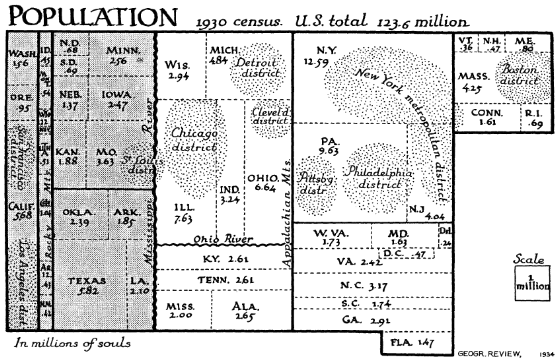
\includegraphics[scale=.5]{introduction/img/cartogram.png}
    \caption{A cartogram by Raisz~\cite{Raisz1934} made in 1934.}
    \label{fig:intro:raisz}
  \end{figure}
  In for example atlases \emph{rectangular cartograms} are used to display information, such as population or economic strength, in a spatial manner.
  In a rectangular cartogram  the geographic regions of an ordinary map are replaced by rectangles; we let these rectangles maintain adjacencies with each other to suggest geographic location and scale them proportionally to the quantities they represent.
  Raisz~\cite{Raisz1934} introduced these cartograms and provided cartograms of, for instance, land area, population (see Figure  \ref{fig:intro:raisz}) and wealth of the United States of America.
  In a rectangular cartogram it is preferable to maintain the adjacencies of the regions that are replaced by rectangles, this in order to keep the representation recognizable.
  However, this is only possible under some conditions as can be seen in Theorhem \ref{th:rect:exsitenceREctangularDual}.
  Note that the cartograms made by Raisz do not keep all adjacenies, for example, in Figure \ref{fig:intro:raisz} Florida and Alabama are not adjacent while they are in reality.

  The value of the displayed quantities, like population or wealth, often changes over time.
  When we draw a set of cartograms displaying a quantity at different moments in time, it is desirable if the adjacencies between these rectangles remain the same, no matter the moment in time.
  Moreover, it would be even better if the nature of these adjacencies, that is whether the rectangles border in a vertical or horizontal manner, does not change.
  This raises the question: When is this possible?

%  Since the size of each region will change according to the moment in time, we need to find a %rectangular cartogram that allows all area assignments.
%  \fxwarning{TODO define area addignment or change this}
%  However, even in this case it is desirable that the nature of the orientations, that is whether %it is horizontal or vertical, does not change over time.
%
%  %TODO Introduce adjeceny graph here?
%  This raises the following questions: "Which adjacency graphs can be faithfully represented by a %rectangular cartogram?" and, "Which adjacency graphs admit a cartogram that has orientations that %remain the same for all assigned areas?"
%  \fxnote{Expand on this}

\mypar{Rectangular layout}
  Mathematically, a rectangular cartogram is a  \emph{rectangular layout} (or simply \emph{layout}).
  A layout $\L$ is a partition of an axis-parallel rectangle into a finite set of interior-disjoint axis-parallel rectangles.
  A rectangular layout that has an combinatorially equivalent layout, regardless the area sizes we assign to each rectangle is \emph{area-universal}.
  \fxnote{Figure of area-universal layouts}
  The question above then becomes: For which maps can we create a area-universal layout?
  It is clear that we must leave out those maps that do not have any layouts with the same adjacencies, but this will not be enough.

\mypar{Adjacency graphs}
  We can represent the adjacencies of map regions by an \emph{adjacency graph} $G$ where each region is represented by a vertex and two vertices are connected by an edge exactly when their regions are adjacent.
  Similarly, in the \emph{adjacency graph} $\dualgraph{\L}$ of a rectangular layout $\L$ each rectangle is represented by a vertex and two vertices are connected by an edge exactly when their rectangles are adjacent.
  A layout $\L$ is a \emph{rectangular dual} of a graph $G$ if we have that $G = \dualgraph{\L}$.
  Rinsma found a graph $G$ in~\cite{Rinsma1987} that has no area-universal rectangular duals.
  That is, all rectangular layouts with $G$ as adjacency graph are not area-universal.

\mypar{One-sided layouts}
  So, unfortunately not all adjacency graphs of map regions admit area-universal duals.
  Then we would like to know which graphs do.
  For this we need to define what a one-sided layouts is.
  Note that the interior of a rectangular layout contains vertical and horizontal line segments.
  Any line segment that can not extended farther on either side is a \emph{maximal segment}.
  Such a layout is \emph{one-sided} if every maximal segment has only one rectangle on one of its sides.
  \fxnote{Figure}
  In~\cite{Eppstein2012} Eppstein et al. show that rectangular layouts are area-universal exactly when they are one-sided.
  So, Rinsma's result also implies that not all adjacency graphs of maps can be represented by an one-sided layout.


\mypar{$\mathbf{k}$-sided layouts}
  Let us consider those graphs that do not admit a one-sided, and thus area-universal, layout.
  Since any layout for such a graph is not area-universal, it is inevitable that adjacencies between regions in this layout change when we are resizing them.
  For these graphs we want to find layouts that have the least number of adjacency changes when area sizes change.
  This is beneficial for, for example, applications displaying cartograms on a continuous timescale.
  Since every time the adjacencies of the layout change, we have to compute a new rectangular layout with the right adjacencies, providing a rougher viewing experience.

  We call a layout \emph{$k$-sided} if $k$ is the smallest integer such that every maximal segment has at most $k$ rectangles on one of its sides. This is a direct generalization of one-sidedness.
  This generalization is useful because, when changing the areas of rectangles in a $k$-sided layout fewer adjacencies change, in general, if $k$ is small then if $k$ is large.

  We illustrate this by comparing a typical $2$-sided and a typical $10$-sided segment.
  Let us first consider the $2$-sided segment in Figure \ref{fig:intro:2sidedBefore}, if the size of $a$ doubles only two adjacencies change, namely $dA$ and $cB$, as can been seen in Figure \ref{fig:intro:2sidedAfter}.
  While for an example of a $10$-sided segment doubling the size of a single rectangle leads to $15$ changed adjacencies, namely $aC\ aD\ bB\ bC\ bD\ bE\ cC\ cD\ cE\ cF\ dE\ dG\ eF\ eH\ fG$, as can been seen in Figure \ref{fig:intro:10sided}.

  Hence we would like to find $k$-sided layouts for all graphs with $k$ as small as possible.

  \begin{figure}[t]
    \centering
    \begin{subfigure}[b]{0.45 \textwidth}
      \centering
      
\includegraphics{introduction/img/2sidedBefore.pdf}
      \caption{Before resizing $a$}
      \label{fig:intro:2sidedBefore}
    \end{subfigure}

    \begin{subfigure}[b]{0.45 \textwidth}
      \centering
      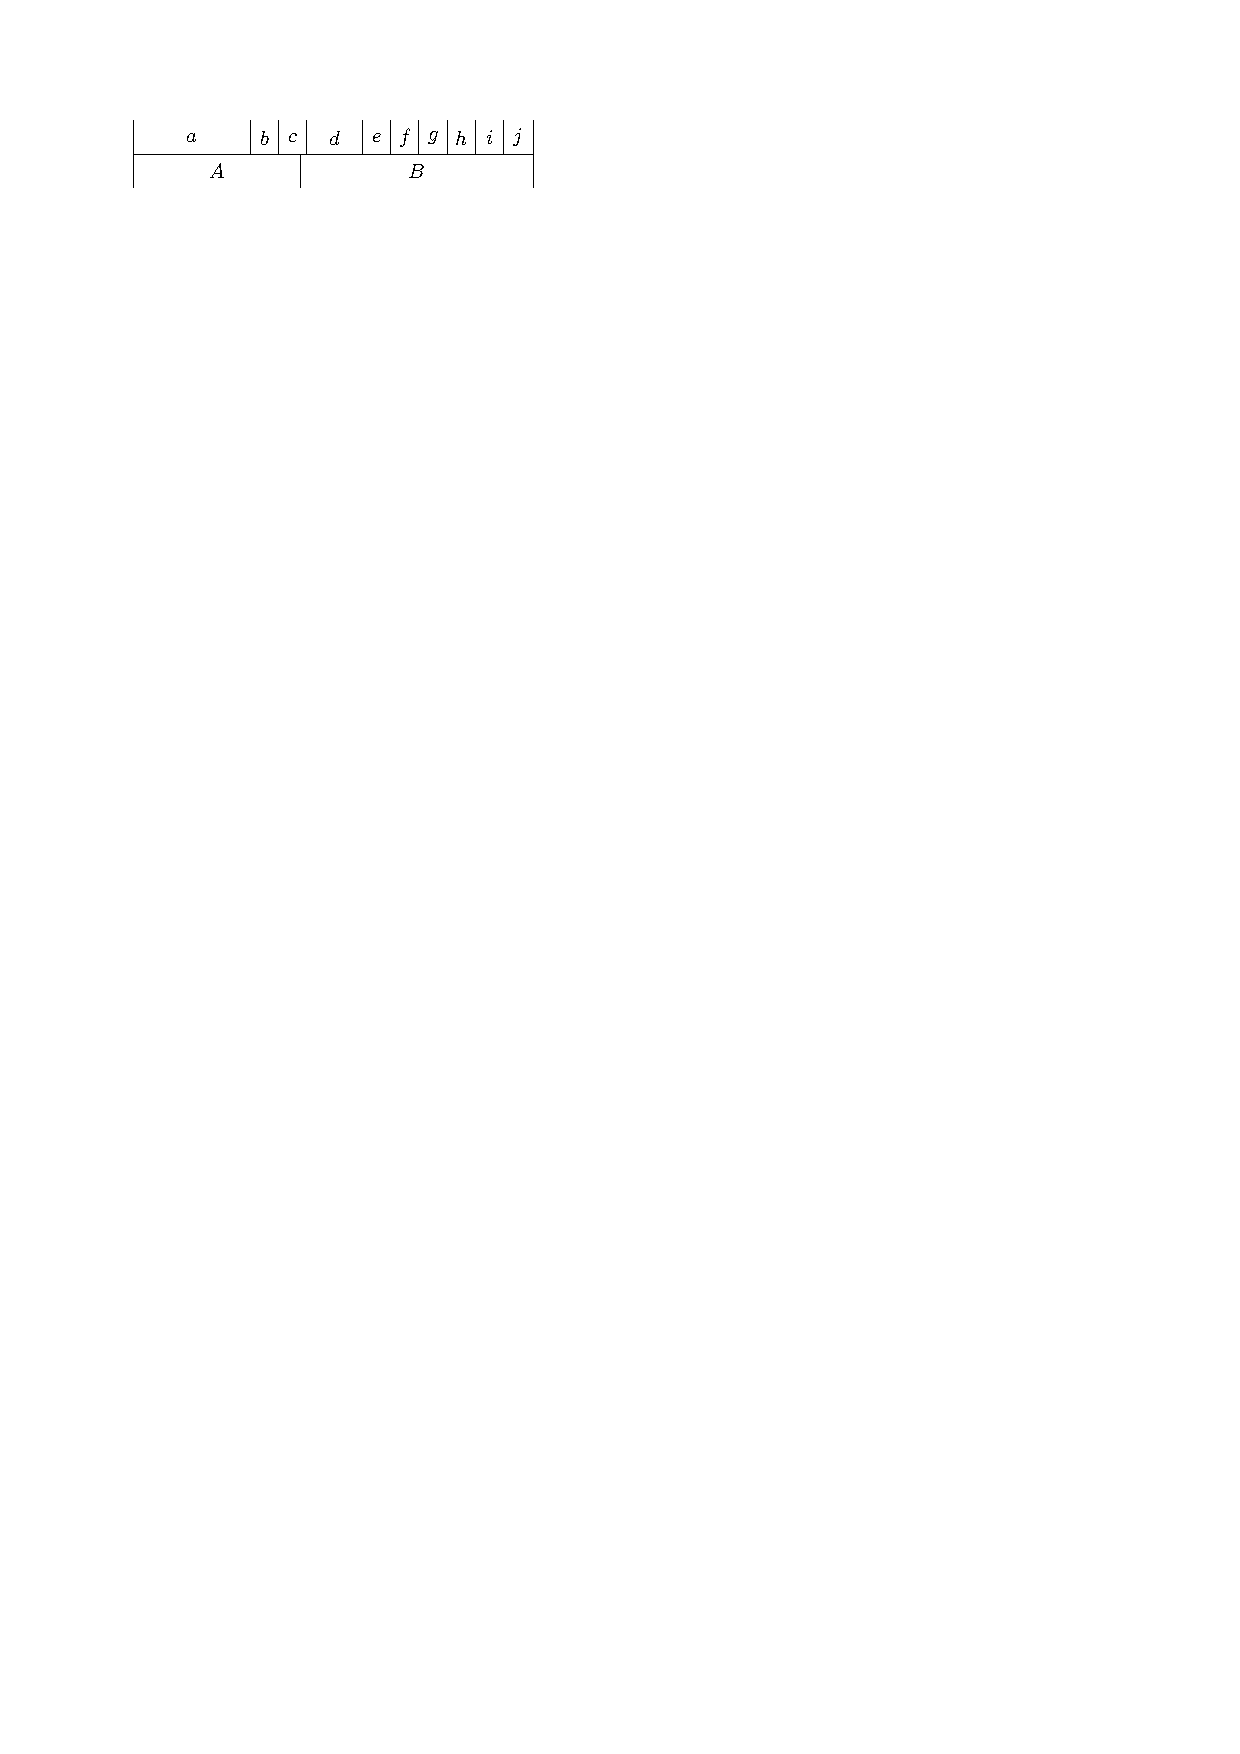
\includegraphics{introduction/img/2sidedAfter.pdf}
      \caption{After resizing $a$}
      \label{fig:intro:2sidedAfter}
    \end{subfigure}
    \caption{A 2-sided segment}
    \label{fig:intor:2sided}
  \end{figure}

  \begin{figure}[b]
    \centering
    \begin{subfigure}[b]{0.45 \textwidth}
      \centering
      
\includegraphics{introduction/img/10sidedBefore.pdf}
      \caption{Before resizing $a$}
      \label{fig:intro:10sidedBefore}
    \end{subfigure}

    \begin{subfigure}[b]{0.45 \textwidth}
      \centering
      
\includegraphics{introduction/img/10sidedAfter.pdf}
      \caption{After resizing $a$}
      \label{fig:intro:10sidedAfter}
    \end{subfigure}
    \caption{A 10-sided segment}
    \label{fig:intro:10sided}
  \end{figure}


\mypar{Counterexample}
  In this thesis we provide two results on $k$-sidedness. The first result is that there is a family of graphs $G_k$ that for any constant $k \in \N$ has members that are not $k$-sided (Theorem \ref{fix:th:family}). The family of graphs in this result is characterized by the occurrence of nested separating $4$-cycles.
  A \emph{$4$-cycle} is a cycle of length $4$.
  Such a cycle is separating if there are vertices in both its interior and exterior.
  Separating $4$-cyles are \emph{nested} if one is contained in the other, but some of their vertices overlap.
  \fxnote{Some example fig of these cycles}
  $4$-cycles in general are difficult to treat but examples indicate that nested $4$-cycles are the most difficult to treat when trying to create a $k$-sided layout.


  \fxnote{BLABLA on 4-cyles in other problems}

\mypar{Corner assignments}
  Before we can state our second result we will have to briefly introduce the concepts of corner assignments.
  A corner assignment $\ext G$ of a graph $G$ is an augmentation of $G$ with $4$ external vertices, which we call its \emph{poles}, with the following three properties (i) every interior face has degree $3$, (ii) the exterior face has degree $4$ and (iii) $\ext G$ has no separating triangles.
  A corner assignment fixes which rectangles are in the corners of the rectangular dual $\L$, namely those adjacent to two poles, which explains the terminology.

\mypar{Algorithm}
  Following the counterexample we found, we focused our efforts on obtaining an algorithm that would provide a $k$-sided layout for corner assignments without a separating $4$-cycle, for some constant $k \in \N$.
  Unfortunately, we fell short of this goal and only found an algorithm that provides a $d-1$-sided layout, where $d$ is the maximal degree of the vertices of $G$ in $\ext G$ (Theorem \ref{th:dsided}).

  That being said, we never found any graph without separating $4$-cycles that did not admit any $2$-sided layouts during our research.
  This raises the conjecture that these graphs in fact do admit a $2$-sided layout and it is just the algorithm for finding them that eludes us.
  \fxnote{show that for example rinsma also satifies this, Figure}

  Its worthy of note, that bound obtained by the algorithm is not stronger then the bound provided by the counterexample. That is, there might be an algorithm providing $O(d)$-sided layouts for all graphs $G$.

\mypar{Combinatorially equivalent}
  We say two layouts are  \emph{combinatorially equivalent} or simply \emph{equivalent} when their rectangles have the same adjacencies with the same orientation(horizontal or vertical) between their rectangles. \fxwarning{Look at definition by speckmann}

  Consider for example Figure \ref{fig:intr:segmentdefs}, the three highlighted lines are all line segments. However, only the red and blue segment are maximal segments. The red segment is one-sided and the blue segment is $2$-sided and the whole layout is $2$-sided. Furthermore, the layout in Figure \ref{fig:intr:vertonesided} is $4$-sided.

  \begin{figure}[b]
      \centering
      \begin{subfigure}[b]{0.45 \textwidth}
        \centering
        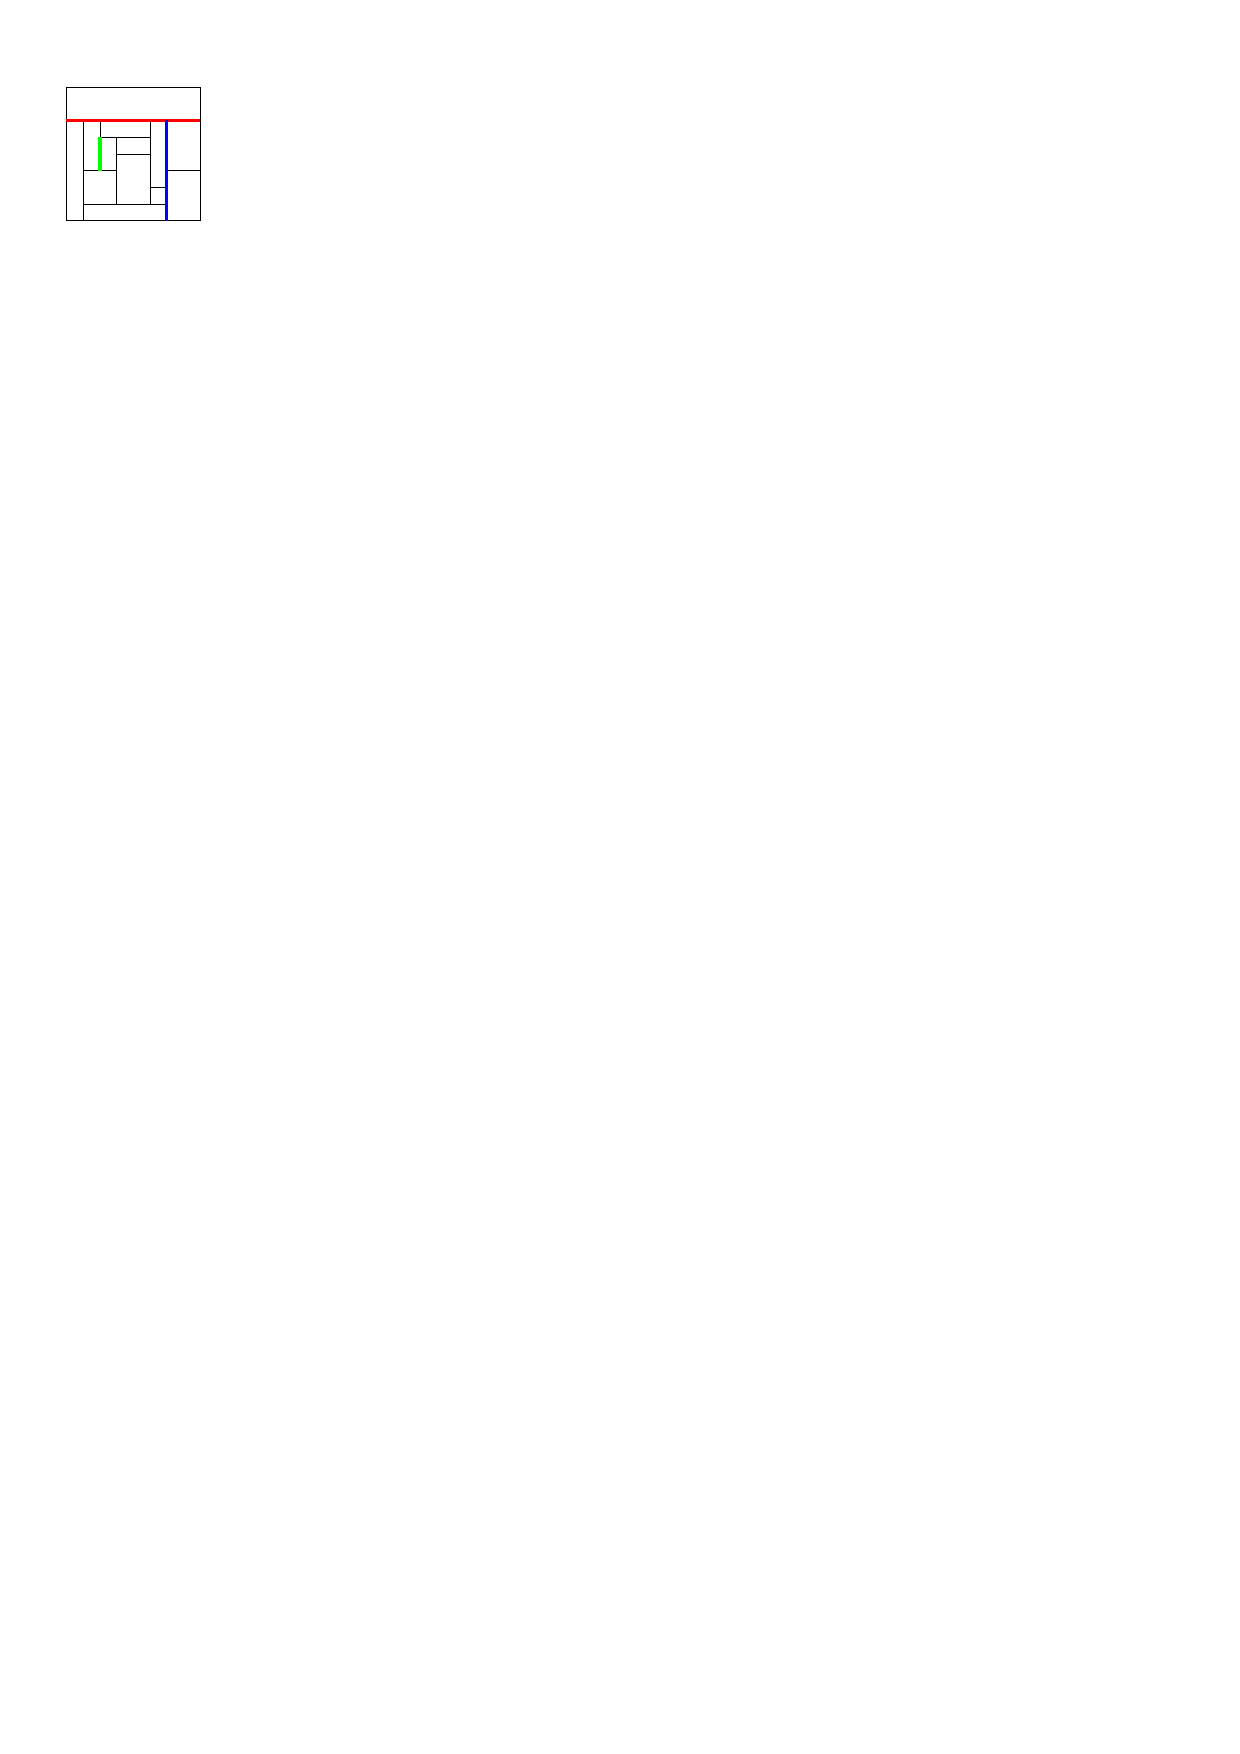
\includegraphics[scale=1]{rectangularDuals/img/segmentdefs}
        \caption{A rectangular layout.}
        \label{fig:intr:segmentdefs}
      \end{subfigure}
      ~
      \begin{subfigure}[b]{0.45 \textwidth}
        \centering
        
\includegraphics[scale=1]{rectangularDuals/img/vertonesided}
        \caption{Another rectangular layout.}
        \label{fig:intr:vertonesided}
      \end{subfigure}
      \caption{Rectangular layouts}
      \label{fig:intr:graphs}
  \end{figure}

\mypar{Graphs}
  A \emph{graph} $G$ is an abstraction of a network. The objects are represented by a set of \emph{vertices}.
  Connections between objects are represented by a set of \emph{edges}; each edge connects two vertices.
  Two distinct edges do not have the same vertices and no edge starts and ends at the same vertex.
  That is, graphs in this thesis are \emph{simple}. An edge is \emph{incident} to a vertex $v$ if that edge connects $v$ to another vertex.
  The \emph{degree} of a vertex is the number of edges incident to this vertex.
  All graphs in this thesis are \emph{planar}.
  That is, they can be embedded in the plane without their edges crossing. A \emph{face} is connected component of the maximal subset of the plane that is disjoint from the embedded graph. The \emph{degree} of a face is the number of vertices on its boundary.
  A face of degree $3$ is a \emph{triangular} face. The \emph{outer face} is the one and only unbounded face.
  A vertex is \emph{incident} to a face when it lies on its boundary.

  All graphs in this thesis are \emph{triangulations of the $k$-gon}. A triangulation of the $k$-gon has an outer face of degree $k$ and interior faces of degree $3$.
  Vertices bordering the outer face are \emph{outer vertices} while all other vertices are \emph{interior vertices}.
  Triangulations of the $k$-gon are called \emph{(plane) triangulated graphs} by some other authors.

\mypar{Rectangular duals}
  Two vertices are \emph{adjacent} when they are connected by an edge. Two rectangles are \emph{adjacent} when their boundaries overlap. A \emph{rectangular dual} of $G$ is a rectangular layout whose adjacencies are the same as those of $G$ for a bijection between vertices and rectangles.

\mypar{Corner assignments}
  If we want to determine which graphs do have a rectangular dual, then we need to introduce the notion of a \emph{corner assignment}.
  A corner assignment $\ext G$ of $G$ is an augmentation of $G$ with $4$ external vertices ,which we call its \emph{poles}, with the following 3 properties (i) every interior face has degree $3$, (ii) the exterior face has degree $4$ and (iii) $\ext G$ has no separating triangles.
  A corner assignment fixes which rectangles are in the corners of the rectangular dual $\L$, which explains the terminology.

  A corner assignment of $G$ only exists if $G$ is a triangulation of the $k$-gon for some $k$. Otherwise, there is no way of adding poles that makes all the interior faces of degree $3$. Because of this, we only consider triangulations of the $k$-gon in this thesis. A corner assignment $\ext G$ of $G$ is an example of a triangulation of the $4$-gon. A corner assignment fixes which rectangles are in the corners of the rectangular dual $\L$, which explains the terminology.

\mypar{Existence and uniqueness}
  Now we can state which graphs admit a rectangular dual. The following result was shown independently by Kozminski and Kinnen \cite{Kozminski1984} and Ungar \cite{Ungar1953}.

  \begin{thrm}[Existence of a rectangular dual]
    \label{th:rect:exsitenceREctangularDual}
    A triangulation of the $k$-gon $\G$ has a rectangular dual if and only if it has a corner assignment without separating triangles $\ext \G$.
  \end{thrm}

  A graph $G$ can have multiple rectangular duals. $G$ can even have duals that are not equivalent. An example is given by the two non-equivalent duals of the same graph given in Figure \ref{fig:intr:graphs}.
  \fxwarning{Add wrapfig this other figure is too big}

\mypar{Rectangular cartograms}
  A rectangular cartogram is the rectangular dual of the adjacency graph of the map $G$.
  If the areas change it might be that a certain rectangular layout can not fulfill its adjacencies anymore and we have to switch to another non-equivalent rectangular dual of $G$.

  We would like to find a rectangular dual that has adjacencies that hold regardless of the area sizes we assign to each rectangle. We say such a dual is \emph{area-universal}.
  Eppstein et al. have shown that rectangular duals are area-universal exactly when they are one-sided.~\cite{Eppstein2012} Unfortunately not all graphs admit a one-sided dual. One such graph, displayed in Figure \ref{fig:intro:rinsma},  is given by Rinsma.~\cite{Rinsma1987}

  \begin{figure}[!t]
    \centering
    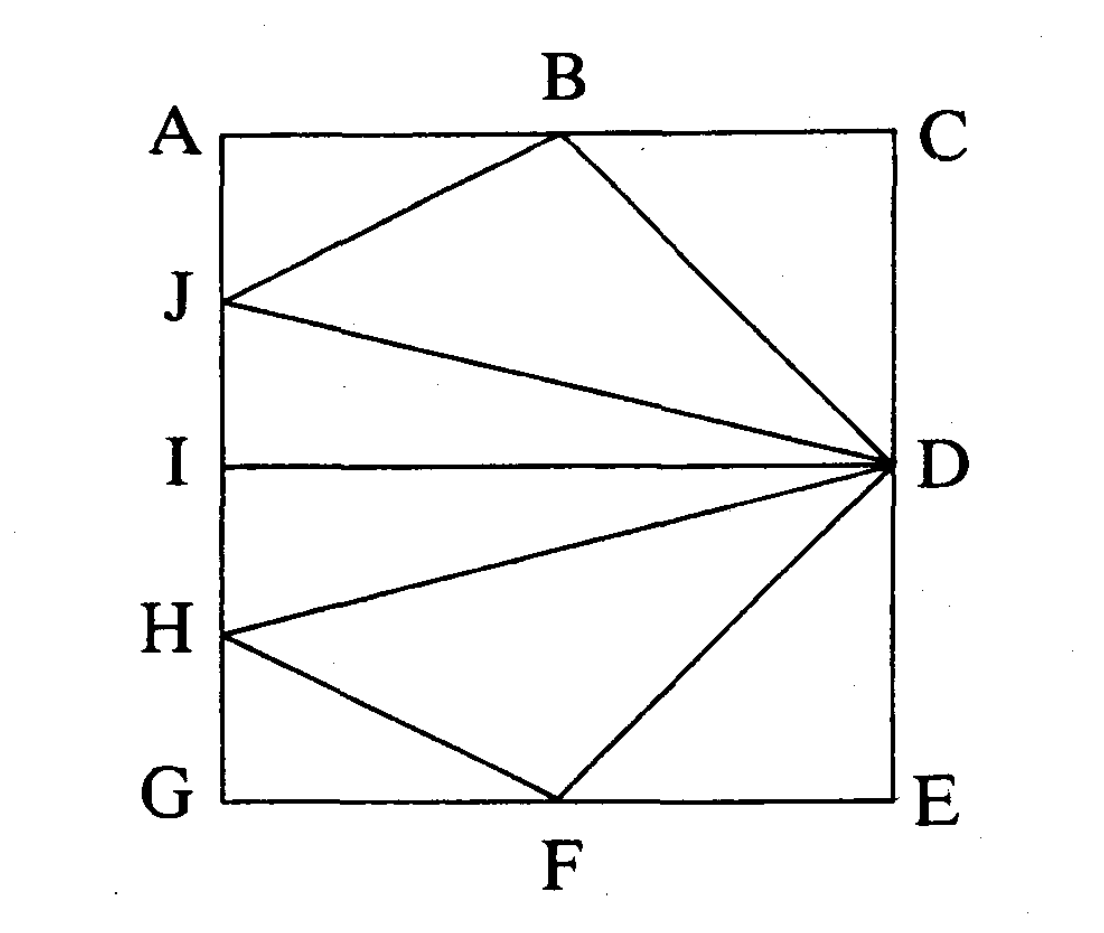
\includegraphics[scale=.15]{introduction/img/rinsma.png}
    \caption{The graph by Rinsma~\cite{Rinsma1987} that is not one-sided.}
    \label{fig:intro:rinsma}
  \end{figure}

\mypar{Overview}
  The rest of this thesis is focused on obtaining these results.
  In order to do this we treat paths and cycles in the remainder of this section. In Section \ref{s:rel} we introduce the notion of regular edge labellings which we use in the rest of the thesis. A regular edge labeling is a way of coloring and orienting the edges of a graph that corresponds to a rectangular dual of that graph.
  Once we have the preliminaries out of the way we prove Theorem \ref{fix:th:family} in Section \ref{s:fix} and Theorem \ref{th:dsided} in Section \ref{s:algo}. The proof of Theorem \ref{fix:th:family} is by counterexample while the proof of Theorem \ref{th:dsided} is provided by giving a constructive algorithm.


\mypar{Paths and Cycles}
  In the rest of the thesis we frequently need paths and cycles, hence we define them here.

  A path $\P$ is a sequence of vertices such that every two consecutive vertices are connected by an edge. The first and last vertex of the path are its \emph{extreme} vertices while the rest are \emph{internal} vertices of this path. The \emph{length} of a path is the number of edges used to connect the vertices. That, is one less than the number of vertices. In this thesis all paths are \emph{simple}, that is, no vertex occurs twice in the path except possibly the extreme vertices.

  A cycle is a path whose extreme vertices coincide. Because a cycle is a path the start and end vertex are the only vertices that occurs more than once. We call a cycle of length $k$  a \emph{$k$-cycle}. A \emph{triangle} is cycle of length $3$ (i.e. a $3$-cycle). By Jordan's curve theorem a cycle splits the plane into two parts, one bounded and one unbounded. We call the bounded part the \emph{interior} of this cycle and the unbounded part the \emph{exterior} of this cycle.
  Furthermore, the cycle of all vertices bordering the outer face is the \emph{outer cycle}.
  We call a cycle \emph{separating} if there are vertices in both its interior and exterior.
  An \emph{interior edge} of a cycle is then an edge contained in the interior of the cycle.
  An \emph{interior path} is a path connecting two distinct vertices off the cycle and whose edges are interior edges.

%\section{Types of triangulations and their properties}
\subsection{Preliminaries}
All graphs are presumed simple and have a fixed planar embedding. In this thesis paths and cycles are always simple while walks are not necessarily simple.

The \emph{degree} of a face is the number of vertices it is incident to. By a \emph{cycle} we will mean a simple cycle. That is a cycle without repetition of edges or vertices. By Jordan's curve theorem a cycle splits the plane into two parts, one bounded and one unbounded. %TODO cite 
We will call the bounded part the \emph{interior} of this cycle and the unbounded part the \emph{exterior} of this cycle.

We will call a cycle \emph{separating} if there are vertices in both it's interior and exterior. We will use \emph{$k$-cycle} to denote a cycle of length $k$. Moreover a \emph{triangle} is simply a cycle of length $3$ (i.e. a $3$-cycle). 


\subsection{Plane triangulations}

\begin{defi} [Plane triangulation]
A graph with only faces of degree $3$.
\end{defi}


\begin{defi} [Maximal planar graph]
A graph such that adding any one edge leaves it non-planar.
\end{defi}

\begin{thrm}
Any graph $G$ is a plane triangulation \ifftext it is maximal planar
\end{thrm}

\begin{proof}
We will prove the equivalence of the negations.

Suppose that $G$ is not maximally planar. Then there is a face $F$ to which we can add an edge, however this face must then have degree larger then $4$. Hence $G$ is also not a plane triangulation. 

Suppose that $G$ is not a plane triangulation. Then there must be a face $F$ of degree larger then $3$. This face will thus admit an extra edge without violating planarity and hence $G$ is not maximally planar.
\end{proof}

\subsubsection{Connectedness}
\begin{thrm}
Any plane triangulation $T$ is $3$-connected.
\label{th:plTri3Connected}
\end{thrm}

\begin{proof}
Suppose that $T$ is not $3$-connected. Then there must be a $2$-cutset $S$, given by the vertices $x$ and $y$. Removing this cutset splits the graph into at least two connected components $C_i$ and all components are incident to all cutvertices otherwise we would have found a $1$-cutset.

Since $S$ is a cutset, there can't be any edges incident to both $C_1$ and $C_2$. But then the edge $xy$ should be separating the $2$ components on both sides. This is impossible since we can only draw this edge once. %TODO figure/ and clarify
\end{proof}

\begin{defi}[Irreducible triangulation]
We call a triangulation irreducible if it has no separating triangles
\end{defi}

%TODO show reduction?

\begin{thrm}
Any irreducible plane triangulation $T$ is $4$-connected.
\end{thrm}

\begin{proof}
Note that any plane triangulation is $3$-connected by Theorhem \ref{th:plTri3Connected}.

Suppose that $T$ is not $4$-connected. Then there must be some $3$-cutset (since it is $3$-connected) let us denote the vertices of this cutset by $x, y$ and $z$. Removing this cutset splits the graph into at least two connected components $C_i$ and all components are incident to all cutvertices otherwise we would have found a $2$- or $1$-cutset.  

However, now $xy$ must be an edge in the triangulation $T$ otherwise the graph is not maximal planar (There can't be an edge incident to both $C_1$ and $C_2$ because that would negate $x, y ,z$ being a cutset.). In the same way $yz$ and $xz$ are edges of $T$. But then $xyz$ is a separating triangle. This is an contradiction and thus $T$ is $4$-connected
\end{proof}

\subsection{Triangulations of the $k$-gon}

\begin{defi}[Triangulation of the $k$-gon]
We call a graph a triangulation of the $k$-gon if the outer face has degree $k$ and all interior faces have degree $3$.
\end{defi}
Vertices bordering the outer face are \emph{outer vertices} while all other vertices are \emph{interior vertices}. Furthermore the cycle formed by all vertices outer vertices is the \emph{outer cycle}.

Sometimes such triangulations of the $k$-gon are called \emph{(plane) triangulated graphs}.


\begin{defi}[Irreducible triangulation of the $k$-gon]
We call a triangulation of the $k$-gon irreducible if it has no separating triangles.
\end{defi}


Note that triangulation of the $n$-gon $n\geq 4$ is not maximally planar and thus not plane triangulation.

\begin{comment}
%Don't know yet if this a usfull construct
\begin{thrm}
The interior of a triangulation of the $n$-gon is maximally planar. That is to say, we can't add any edges except trough the outer face.
\end{thrm}

\begin{proof}
Suppose the 
%TODO (not max plan. => face of degree 4
\end{proof}
\end{comment}

The \emph{completion} of a triangulation of the $k$-gon $G = (V, E)$. Is the graph $G'= (V', E')$ with vertex set $V' = V \cup \braces{s}$ and edge set $E' = E \cup \braces{ sv | v \text{ is a outer vertex}}$ 

The completion is plane triangulation.  %Q does this stament need proof? 
Since the interior of the outer cycle of $G$ always consisted of faces of degree 3. The exterior of the outer cycle consisted of one face of degree $k$ (the outer face) but the completion has turned this into $k$ faces of degree $3$.  

\begin{thrm}
A triangulation of the $k$-gon $G$ is $2$-connected.
\end{thrm}
\begin{proof}
Suppose that $G$ has a cutvertex $v$. Then the set $\braces{s, v}$ is a $2$-cutset of the completion $G'$ of $G$. This however is in contradiction to Theorem \ref{th:plTri3Connected} stating that $G'$ is $3$-connected. Hence $G$ has no cutvertex and is thus $2$-connected.
\end{proof}

\begin{thrm}
\label{th:irreducible and chordless triangulation of the kgon is 3connected}
A irreducible and chordless triangulation of the $k$-gon is $3$-connected.
\end{thrm}
\begin{proof}
\note Will be provided if this statement turns out to be interesting. Will go via the fact that the completion is a irreducible triangulation. Chordless outer cycle is important, because a chord will form a separating triangle in $G'$.
\end{proof}

\begin{thrm}
Any irreducible triangulation $T$ of the $4$-gon with $n \geq 5$ is $3$-connected. 
\end{thrm}

\note This proof could be a corrolary of the above theorhem \ref{th:irreducible and chordless triangulation of the kgon is 3connected}. A chord gives a separating triangle if $n\geq 5$.
\begin{proof} 
Let us name the four outer vertices $a,b,c,d$ in clockwise order. Let us first note that the diagonals $ac$ and $bd$ can't be an edge since this would create a separating triangle containing the $5$th vertex. Let $I$ denote the component of all interior vertices, since every face in the interior is of degree $3$ each outer vertices is incident to at least one edge that is also incident to $I$. %TODO figure

One can now easily check that there is no $2$cut set with only exterior vertices. However, a cutset with $1$ or $2$ interior vertices leads to at least one cycle of degree greater then $3$ %TODO expand/ figure.

Hence no $2$-cutset of $T$ can't exist and $T$ is $3$-connected. 
\end{proof}

\begin{thrm}
For every interior vertex $v$ of a triangulation of the $k$-gon $G$ is connected by ate least $3$ vertex disjoint paths to different outer vertices.
\end{thrm}
\begin{proof}
By Theorhem \ref{th:plTri3Connected} the completion $G'$ of $G$ is $3$-connected. Hence there are 3 vertex-disjoint paths from $v$ to $s$. Since $v$ is on the interior and $s$ is on the exterior of the outer cycle $\C$ all these 3 paths cross the outer cycle at least once. These paths cross $\C$ for the first time in different vertices since they are vertex-disjoint. If we shorten the paths to their first crossing with $\C$ we obtain the $3$ paths in the theorem.
\end{proof}

\note We can sharpen this to $4$ if we have a irreducible an chordless triangulation of the $k$-gon

\begin{thrm} 
Every interior vertex of a triangulation of the $n$-gon has degree at least $3$.
\end{thrm}
\begin{proof}
Suppose a interior vertex $v$ has degree $1$ then clearly the face surrounding $v$ can't have degree $3$. Now suppose that an interior vertex $v$ has degree $2$. We then let $u$ and $w$ denote it's neighbours and $F$ and $F'$ the face incident to $v$. See also Figure \ref{fig:interiorVertexDegree3}. Then since $F$ and $F'$ are both interior faces they need to be off degree $3$ this implies that $uw$ is an edge for both faces. This is impossible and hence every interior vertex has at least degree $3$
\end{proof}

\begin{figure}[h!]
\centering
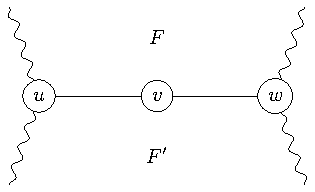
\includegraphics{prelim/img/interiorVertexDegree3.pdf}
\caption{The notation as described in the proof \label{fig:interiorVertexDegree3}
}
\end{figure}

\note If we forbid irreducible triangulations every interior vertex is of degree $4$ since the neighbourhood of any internal vertex $v$ looks like a set of triangles.

\note This theorem is currently (17-09) unused.




\section{Rectangular duals}

\newcommand{\G}{\scr G}
\renewcommand{\L}{\scr L}

In this section we will explain what we mean with the rectangualr dual of a graph. We will prove some simple properties of graphs and their duals.

We define a \emph{rectangular layout} (or simply \emph{layout}) $\L$ to be a partition of a rectangle into finitely many interiorly disjoint rectangles. 

We will assume that no four rectangles meet in one point.

We will then look at the \emph{dual graph of a layout} $\L$ and denote this graph by $\G(\L)$. That is, we represent each rectangle by a vertex and we connect two vertices by an edge exactly when their rectangles are adjacent. Note that this graph is not the same as the \emph{graph dual} of $\L$ when we view it as a graph (namely we don't represent the outer face of $\L$ by a vertex).

So $\G(\L)$ is the dual graph of a layout $\L$. In the reverse direction we say a layout $\L$ is a \emph{rectangular dual} of a graph $\G$ if we have that $\G = \G (\L)$.

A plane triangulated graph $\G$ does not necessarily have a rectangular dual nor is this dual necessarily unique.
%TODO in what sense not unique
%TODO provide examples

%TODO weave a corner assignment in here somewhere

\subsection{Extended graphs}
A \emph{extended graph} $\ext G$ of $G$ is a augmentation of $G$ with $4$  vertices (which we will call it's \emph{poles}). Such that 
\begin{enumerate}
\item every interior face has degree $3$ and the exterior face has degree $4$.
\item all poles are incident to the outer face
\item $\ext\G$ has no separating triangles (i.e separating $3$-cycles).
\end{enumerate}.

We sometimes call an extended graph $\ext G$ of $G$ an \emph{extension} of $G$.

Such a extended graph does not necessarily exist and is not necessarily unique.  %TODO show this
However we have the following result due to .... %TODO cite

\begin{thrm}[Existence of a rectangular dual]
A plane triangulated graph $\G$ has a rectangular dual \ifftext it has an extension $\ext \G$
\end{thrm}

\begin{proof}
Kozminski \& kinnen and ungar, See siAM paper %TODO check this
\end{proof}

We call any (plane triangulated) graph $G$ that has an extension a \emph{proper} graph.

A proper graph $G$ can have more then one extensions. Each such extension fixes which of the rectangles are in the corners of the rectangular dual $\L$. Hence sometimes such an extension is called a \emph{corner assignment}.


\subsection{Regular edge labeling}
A regular edge labelling  of $\ext G$ corresponds to a rectangular dual $\L$ of $G$ with some \emph{corner assignment} fixed. %TODO KANT HE
%explain equivalence

Or regular edge labelling of a graph.


An \emph{interior edge} of a cycle is an edge on the interior of the cycle (when the cycle is viewed as Jordan curve).


\subsubsection{Being onesided in terms of REL}

\subsubsection{Being psudeo-onesided in terms of REL}

\section{Fixing a extension}
In our explorations to find a lower bound on what kind of \emph{psuedo one-sidedness} is possible we will find it very useful to fix one particular extension $\ext G$ of $G$. Unfortunately if there is no rectangular dual that’s $(k,l)$-sided using the \emph{corner assignment} provided by some extension $\ext G$. This does not imply that $G$ is not $(k,l)$-sided. There might be another extension of $G$ such that under the corner assignment corresponding to this extension $G$ has a $(k,l)$-sided rectangular dual. 

Fortunately for us however we can view $\ext G = H$ as a graph in it's own right, then $G$ is the interior of a separating $4$-cycle of $H$ and we will show this implies that $G$ (as induced sugraph) has to be coloured according to the extension $\ext G$. 

\begin{remark}
\label{re:interiorRectangle}
Let $\C$ be a separating $4$-cyle of $G$ with interior $I$. Then in any rectangular dual of $G$ the region enclosed by the rectangles dual to the vertices in $\C$ is a rectangle.
\end{remark}

\begin{remark}
\label{re:disjointRectanglesOnlyHaveOneAdjecentSide}
Two disjoint rectangles are at most adjacent on one side.
\end{remark}

\begin{lemma}
\label{lem:fourCycleUnicolor}
Let $\C = \braces{a, b, c, d}$ be a separating $4$-cyle of $\ext G$ with interior $I$. Then all interior edges incident to $a, b, c$ and $d$ respectively are red, blue, red and blue or blue, red, blue and red.
\end{lemma}

\begin{proof}
%from page 4
%We could also try a reduction along the lines of min. seperation componenets Epstein et. al
By Remark \ref{re:interiorRectangle} the union of the rectangles in the interior of $\C$ will be some rectangle in any rectangular dual. We will denote this rectangle by $I$. Since two disjoint rectangles can only be adjacent to each other at one side all interior edges incident to any vertex of $\C$ are of the same color. 

Furthermore $a, b, c, d$ are all adjacent to a different side of $I$ since $I$ has four sides that need to be covered and it is only adjacent to four rectangles. If we then apply the rules of a regular edge labelling we see that if the interior edges of $a$ are one color, those incident to $b$ and $d$ should have the second color. Then of course the interior edges incident to $c$ are again coloured with the first color. 

\end{proof}

This lemma implies that any \emph{alternating 4-cycle} %TODO define
is either \emph{left-alternating} or \emph{right-alternating} %TODO define
in the terminology of \Fusy

Furthermore the above Lemma is also very useful in that it allows us to fix a extension $\ext G$ of $G$ by building a \emph{scaffold}. Suppose we want to investigate some extension $\ext G$ of $G$ with poles $N$, $E$, $S$ and $W$ then we can consider the graph $\ext G = H$ as a graph in it's own right. $H$ is a proper graph since it has no irreducible triangles in it's interior (because $\ext G$ had none) and it admits a valid extension $\ext H$ by connecting the new poles $NE, SE, SW$ and $NW$ to $N, E, SE, NW$, $S, E, NE, SW$, $S, W, SE, NW$ and $N, W, NE, SW$ respectively. See Figure \ref{fig:scafold} for this extension.  
\fxnote{Maybe use a table}

\begin{thrm}
\label{th:fixExtension}
We can fix an extension, if we want.
\end{thrm}

\begin{figure}[h!]
\centering
\includegraphics[scale=0.5]{prelim/img/scafold}

\caption{The construction of a scaffold. $G$ is displayed in thick lines and with closed vertices. An arbitrary extension $\ext G =H$ is then drawn with thin lines and open vertices. An extension of $H$ is then drawn with dashed edges and open vertices. 
    \label{fig:scafold}}
\end{figure}

The graph $H$ can have more then one extension but they all contain the separating $4$-cycle $\C= NESW$ thus by Lemma \ref{lem:fourCycleUnicolor} we see that, without loss of generality, the interior edges of $\C$ incident to $N$ and $S$ are coloured red and those incident to $E$ or $W$ are coloured blue. This is exactly as if we forced the extension $\ext G$

\subsection{An aplication: There are graphs that are $(2, \infty)$-sided}

We will show this by providing an example graph $G$ with a fixed extension $\ext G$ which we can do according to Theorem \ref{th:fixExtension}. Consider the graph in Figure \ref{fig:2manysidedLowerBound}. Note that most of the interior vertices are of degree $4$ and thus the largest part of any regular edge labelling is forced. Those edges that are forced to have a certain color are already coloured in Figure \ref{fig:2manysidedLowerBound}.


\begin{figure}[h!]
\centering
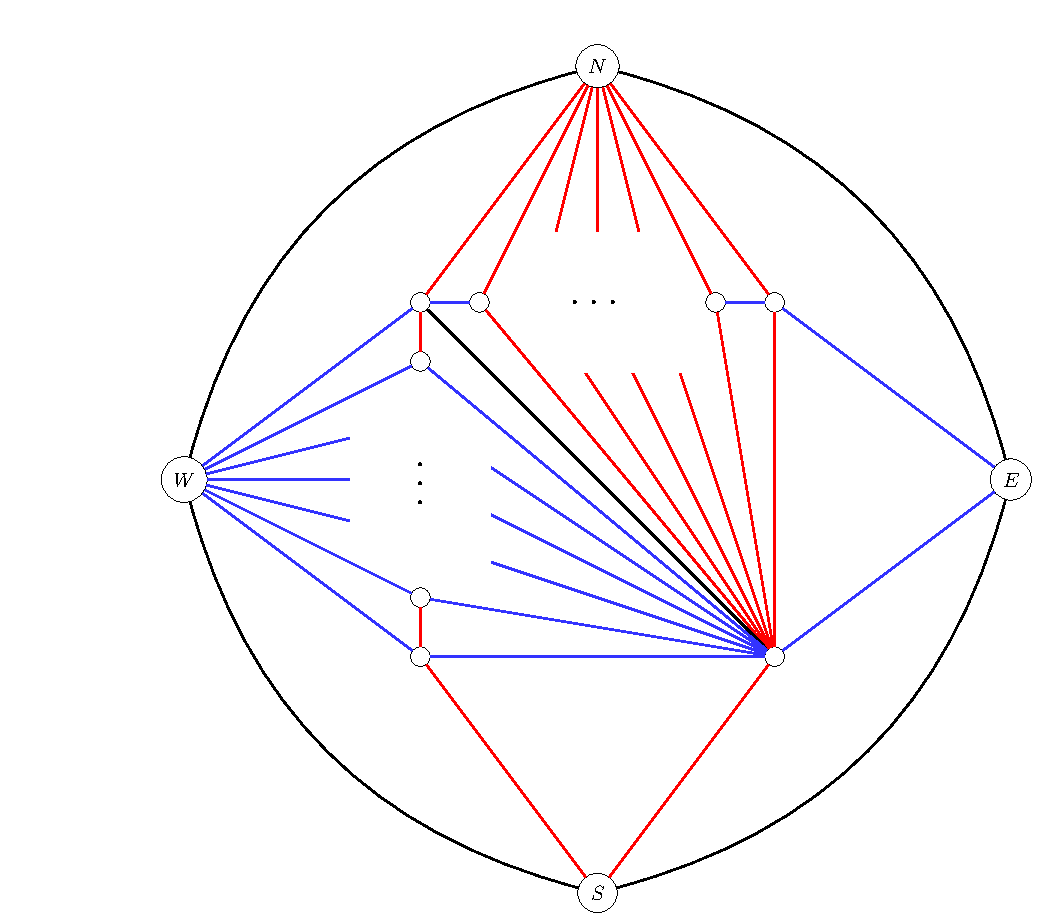
\includegraphics[scale=.5]{prelim/img/2manysidedLowerBound}

\caption{The fixed extension $\ext G$
    \label{fig:2manysidedLowerBound}}
\end{figure}

The only edge for which we have freedom to choose a color is the diagonal edge of $G$. Howeever, if we color this edge blue we get a red $(2, \infty)$ cycle and if we color this edge red we get a blue $(2, \infty)$ cycle. In both cases we will thus obtain a $(2,\infty)$-sided segment in our dual.


%!TEX root = ../thesis.tex

\section{Rectangular duals}
\newcommand{\G}{\scr G}
\renewcommand{\L}{\scr L}

In this section we will introduce the rectangular dual of a graph.

\subsection{Rectangular layouts and their duals}
  We define a \emph{rectangular layout} (or simply \emph{layout}) $\L$ to be a partition of a rectangle into finitely many interiorly disjoint rectangles such that no four rectangles meet in one point.

  We say two layouts are  \emph{combinatorially equivalent} or simply \emph{equivalent} when they have the same adjacencies with the same orientation(horizontal or vertical) between their rectangles.

\subsection{Duals of rectangular layouts}
  In the \emph{dual graph} $\dualgraph{\L}$ of a layout $\L$ we represent each rectangle by a vertex and we connect two vertices by an edge exactly when their rectangles are adjacent.

  One can also consider the \emph{extended dual graph} $\extdualgraph{\L}$ of a layout $\L$. In such a graph we not only represent each rectangle by a vertex. But furthermore we also add $4$ vertices $\pN, \pE, \pS, \pW$ (so-called \emph{poles}) in the outer face, one associated to the north, east, south, west boundary segment of the outer rectangle respectively. Two vertices are then connected if their rectangles or boundary segments intersect.

  If we take the \emph{extended dual graph} of a layout and remove the $4$ vertices corresponding to the outer face we end up with the \emph{dual graph} of that layout.

  Let us note that both the dual graph and the extended dual graph of a layout $\L$ are not the same as the \emph{graph dual} of $\L$ when we view it as a graph (namely we don't represent the outer face of $\L$ by a single vertex).

\subsection{Rectangular dual}
  We have introduced two ways to define the dual $G$ of a layout $\L$. In the reverse direction we say a layout $\L$ is a \emph{rectangular dual} of a certain graph $G$ if we have that $G = \dualgraph{\L}$.

  A triangulation of the $k$-gon $\G$ does not necessarily have a rectangular dual nor is this dual necessarily unique. When existence is guaranteed can be seen in Theorem \ref{th:rect:exsitenceREctangularDual}

\subsection{Different kinds of rectangular layouts}
  We can pose different restriction on a rectangular layout $\L$. For all these restrictions we have that if they hold for one layout $\L$ they hold for all equivalent layouts.

  We will call $\L$ \emph{area-equivalent} if no matter the areas we assign to the rectangles of $\L$ there is a equivalent layout $\L'$ such that each rectangle has the assigned area.
  \fxnote{Might add supporting figures}

  All other restrictions we introduce here will consider the \emph{maximal line segments} (or simply \emph{maximal segement}) of $\L$. A \emph{line segment} (or simply \emph{segment}) of $\L$ is a sequence of consecutive inner boundary segments forming a line. Such a segment is called maximal if it's not contained in any other line segment. \fxnote*{Is this neccesary?}{This notion is also introduced in \cite{Eppstein2012}}. A segment is \emph{one-sided} if it is on the boundary of a single rectangle. We call it \emph{$k$-sideded} if on one of the sides it is the boundary of at most $k$ rectangles. Finally, a line segment is \emph{$(k,l)$-sided} with $k<l$ if the line segment is on the boundary of at most $k$ different rectangles on one side and at most $l$ different rectangles on the other side.
  \fxnote{Might add supporting figures}
  \fxwarning{Think about removing defi for $(k,l)$ sideds, this will proc a rewrite}

  We will then call a layout \emph{one-sided} if all maximal segments are one-sided. Furthermore it is called \emph{vertically one-sided} or \emph{horizontally one-sided} if just all vertical or horizontal maximal segments are one-sided. Furthermore a layout is \emph{$(k,l)$-sided} if all maximal line segments are $(k,l)$-sided.

  Eppstein et al. \cite{Eppstein2012} show that a layout is area-universal if and only if it is one-sided.

\subsection{Regualar edge labeling}
  The extended dual of a layout allows a natural coloring and orientation of its edges. This \emph{regular edge labeling} can be found in the following way:
  For every edge $vw$ in $\extdualgraph{\L}$ we consider whether the shared boundary of the rectangles is vertical or horizontal we then color the edge blue or red respectively. In the first case we orient the edge from the  leftmost point to the rightmost point and in the second case we orient from bottom to top. We don't color or orient the edges between the poles.

  From the nature of the adjacencies in a rectangular layout we can deduce the following two rules for a regular edge labeling.
  \begin{enumerate}
    \item (Interior vertex) In the rotation around every interior vertex we have the following subsequent non-empty sets: Incoming red edges, incoming blue edges, outgoing red edges and outgoing blue edges. And only these sets.
    \item (Pole) $\pN$ has only incoming red edge, $\pE$ has only incoming blue edges, $\pS$ has only outgoing red edges and $\pW$ has only outgoing blue edges. Except for, of course, the uncolored edges between poles.
  \end{enumerate}

  Regular edge labeling were first introduced by Kant and He \cite{Kant1997} and were also used in \cite{Eppstein2012}. Fusy also studied these structures \cite{Fusy2006,Fusy2009} but he calls them \emph{transeversal structures}.

  He showed \cite{He1993} that given a regular edge labeling we can reconstruct a rectangular layout giving this regular edge labeling.

  A regular edge labeling  of $\ext G$ corresponds to a equivalence class of rectangular layouts $\L$ that are a rectangular dual of $G$.

  Note that we have no monocolored directed cycles because such a cycle would for example correspond to a  group of adjacent rectangles that have  no leftmost or topmost one. This is clearly absurd.

  \begin{lemma}
    \label{lm:rel:noMonoColoredTriangles}
    A regular edge labeling doesn't admit a monocolored triangle
  \end{lemma}

  \begin{proof}
    Suppose we have a mononcolored triangle. Without loss of generality we will suppose that the color of this triangle is blue. Then at least one of the vertices has an incoming blue edge followed directly by an outgoing blue edge or an outgoing blue edge followed directly by an incoming blue edge in it's rotation. Thus this vertex has either an empty set of outgoing or incoming red edges, offending the coloring requirements of a REL
  \end{proof}

  \subsubsection{$st$-planar graphs}
    Kant and He \cite[pp.179]{Kant1997} show that an regular edge labeling is closely linked to a pair of $st$-planar graphs. As can be seen in Theorem \ref{th:rel:stPlanarGraphs} below.

    A $st$-planar graph is an oriented planar graph with one source (indegree 0) $s$ and one sink (outdegree 0) $t$. Both $s$ and $t$ lie on the outer face. Moreover, such a $st$-planar graph has no directed cycles.

    \begin{thrm}
      \label{th:rel:stPlanarGraphs}
      The blue edges of $G\sm{\pN,\pS}$ form a $st$-planar graph with $s= \pW$ and $t=\pE$. Moreover the red edges of $G\sm{\pW,\pE}$ form a $st$-planar graph with $s= \pS$ and $t= \pN$.
    \end{thrm}
    \begin{proof}
      Kant and He propose to add an edge and orient the outer cycle. This is necessary because they require $s$ and $t$ to be adjacent. Moreover they don't a priori require such an graph to be without directed cycles.

      A trivial adaptation of \cite[pp.179]{Kant1997} then gives us the theorem. We note that we can't get any directed cycles since a regular edge labeling has no monocolored directed cycles.
      \fxnote{We might write our own proof.}
    \end{proof}

    We will refer to these $st$-planar graphs as the \emph{blue graph} and \emph{red graph} of some regular edge labeling. We will then refer to the faces of these graphs as \emph{blue faces} and \emph{red faces}.

    Every face $F$ in an $st$-planar graph has the same structure. The boundary of $F$ consists of two directed paths with common origin $\spl(F)$ and  destination $\mrg(F)$.\fxnote{We might want to prove this.}
    These boundary paths are adjacent in the orientation at $\spl(F)$. We will say the first path in the rotation, starting at the beginning of the adjacent pair, is the \emph{right boundary path} or \emph{bottom boundary path} of $F$ and the second one is the \emph{left boundary path} or \emph{top boundary path}.

    \subsubsection{Fans}
    We introduce some more concepts to describe the interior of a blue (or red) face. Every interior edge of this face goes from one fence to the other (otherwise it's start or end vertex would offend the interior vertex condition).\fxnote{This could be a useful result in the section about cycles and their interiors.} To better understand the structure of such a strip we will describe the edges from $\spl(F)$ to $\mrg(F)$ .

    Let $u_0 , u_1, \ldots u_n$ be the vertices of the upper boundary path of $F$ and $v_0, v_1, \ldots, v_m$ the vertices of the bottom boundary path. That is $u_0=v_0 = \spl(F)$ and $u_n = v_m = \mrg(F)$. Since our graph is a triangulation $u_1v_1$ must be an edge. For the second edge in the face we have two options $u_1v_2$ or $u_2v_1$, otherwise this edge and the previous one would not form a triangle. This principle holds for every subsequent edge, we can either increase a the index of the upper boundary path or the index of the bottom boundary path. In other words, this face is a so-called \emph{triangle strip}.

    We will call a maximal sequence of at least two edges increasing the index on the bottom boundary path (and thus keeping the index on the upper path fixed) a \emph{Bottom-fan} or simply \emph{B-fan} and a maximal sequence of at least two edges increasing the index on the upper boundary path will be called a \emph{Top-fan} or just \emph{T-fan}. The \emph{size} of such a fan is the number of edges contained in the sequence. By the definition of a fan it has size of at least $2$.
    We will simply use \emph{fans} to refer to both these \emph{types} of fans (i.e. T- and B-fans).

    We will call a fan of size $3$ or larger a \emph{large fan}. Then it is only natural that we call a fan of size $2$ a \emph{small fan}.

    In a strip we alternately encounter B- and T-fans. Since if we would have two adjacent fans of the same type we would just have a single larger fan of that type.
    In Figure \ref{fig:uni:fans} we see a strip consisting of subsequently a B-fan of size $3$, a T-fan of size 2, a B-fan of size $2$, a T-fan of size $6$, a B-fan of size $3$ and a T-fan of size $3$.

    \begin{figure}[h]
      \centering
      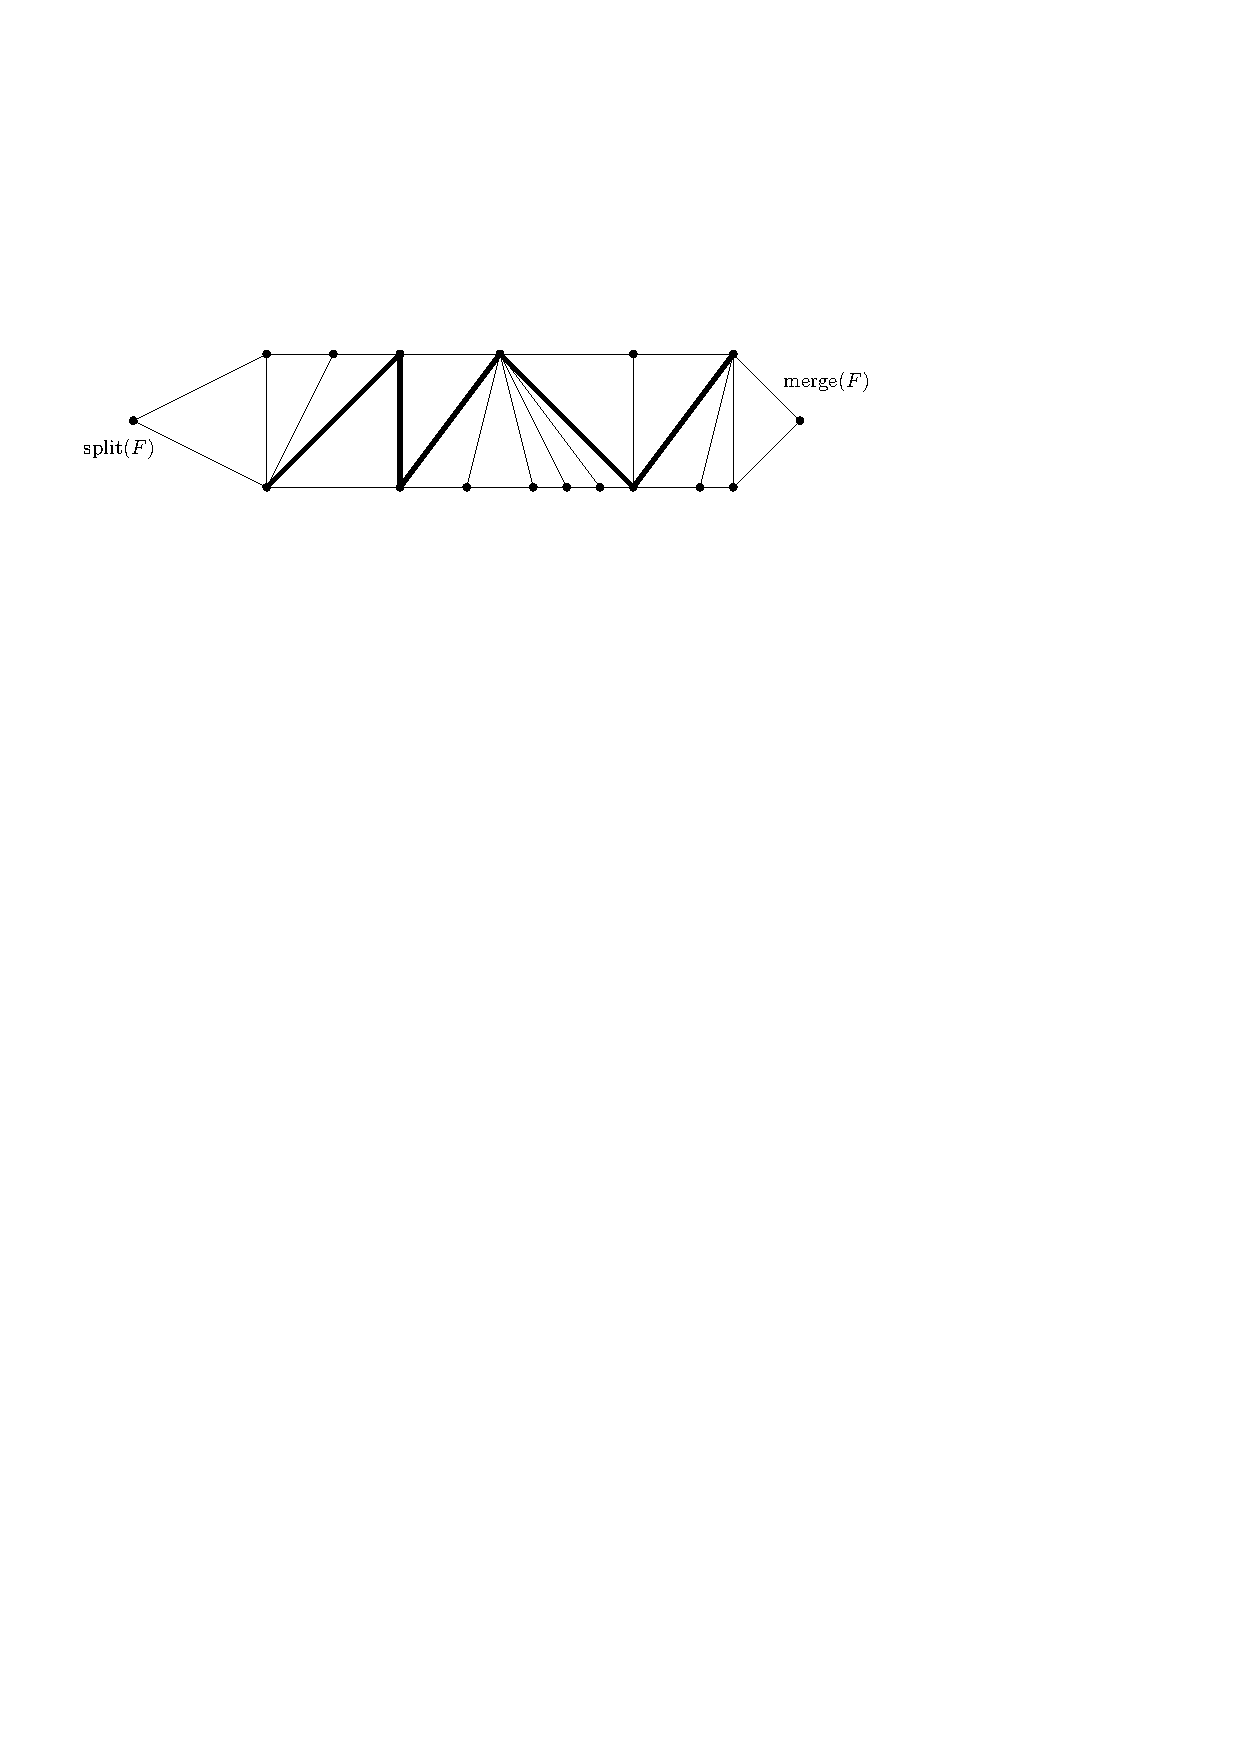
\includegraphics[scale=.9]{rectangularDuals/img/fans}
      \caption{}
      \label{fig:uni:fans}
    \end{figure}


   We introduce some more terminology for fans: \emph{outer edges}, \emph{fan handles} and the \emph{rim} as can be seen in Figure \ref{fig:rect:fanTerms}. The \emph{fan handle} is the vertex shared by all edges in the fan. The \emph{rim} is the path between the vertices of each edge that is not the fan handle. The \emph{outer rim} are the two extreme edges of this path and the \emph{outer edges} are the edges between the fan handles and the extreme vertices of the \emph{rim}.

   \begin{figure}[h]
     \centering
     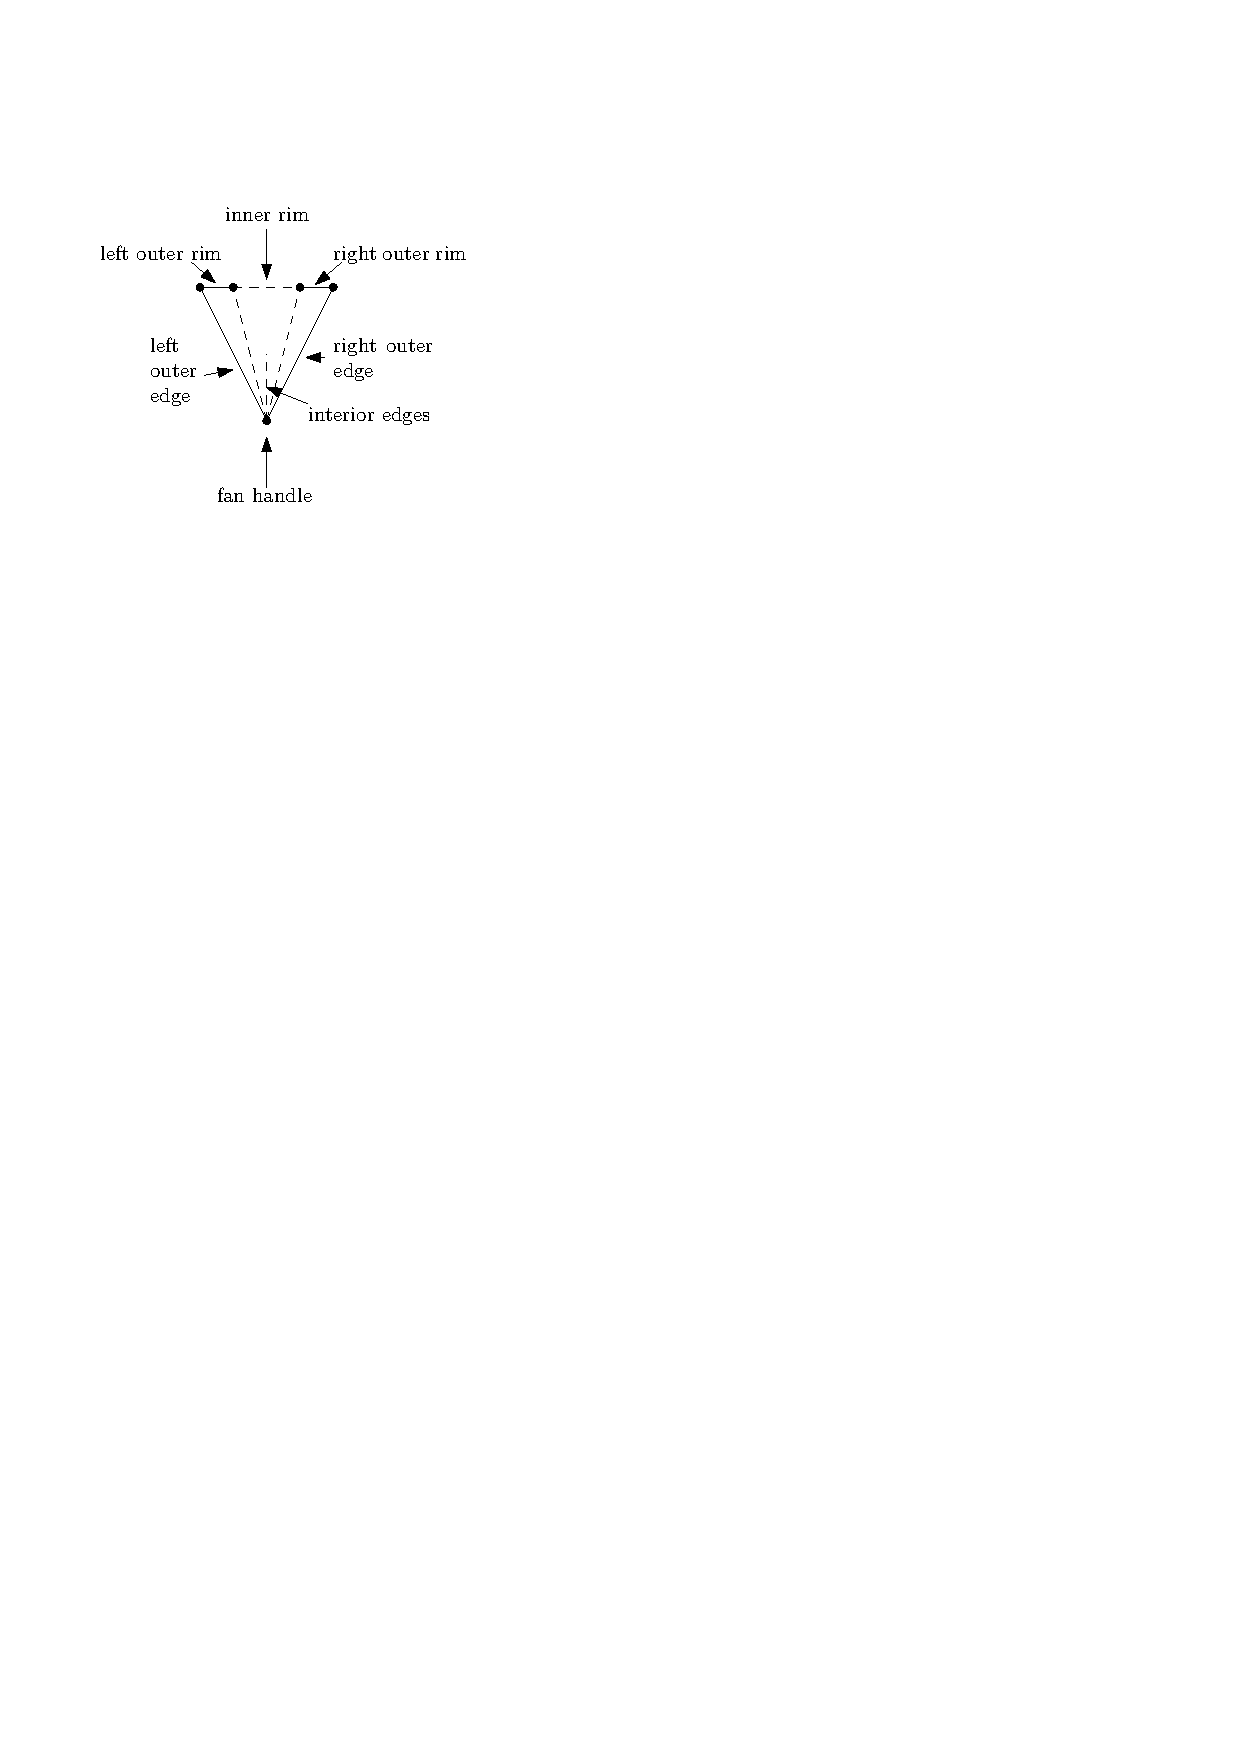
\includegraphics[scale=1]{rectangularDuals/img/fanterms}
     \caption{}
     \label{fig:rect:fanTerms}
   \end{figure}

  \subsubsection{Regular edge labellings and maximal segments}
    From the way that we color a \rel for a given layout $\L$ we can see that a horizontal maximal segment leads to a blue face and a vertical maximal segment leads to a red face.
     \fxwarning{TODO figure of blue face and red face}

    For either type of maximal segment we denote the corresponding face with $F$. The number of interior vertices of both boundary paths without $\mrg(F)$ and $\spl(F)$ is the number of rectangles on the respective sides of the maximal segment.

    Hence a one-sided maximal segment corresponds to a face with one boundary path of length $2$\footnote{A boundary path can't have length $1$ since by construction of a \rel it encloses a maximal segment and thus has to go trough at least one intermediate rectangle/vertex.}. And a $(k,l)$-sided maximal segment has a short boundary path of length at most $k+1$ and a longer boundary path of length at most $l+1$\footnote{Recall that the length of a path its edgecount.}.
    We will for the ease of the discussion ofter refer to such a face as an $(k,l)$-face.

    The following Lemma will prove to be of use
    \begin{lemma}
    \label{lm:zInRedFace}
    A face $F$ with at least $3$ edges on each side contains a $Z$
    \end{lemma}
    \begin{proof}
    \fxerror{TODO}
    \end{proof}

\subsection{Corner assignments}
  \fxwarning[inline, nomargin]{might want to move this to the next section}
  Given a layout $\L$ we can thus easily find the (extended) dual. However finding a rectangular dual of a plane triangulated graph $G$ is more involved. Due to the algorithm by He \cite{He1993} this boils down to finding a regular edge labeling of $G$ with $4$ additional vertices $\pN, \pE, \pS, \pW$. We will define $G$ and these $4$ additional vertices to be a \emph{corner assignment} of $G$.

  \begin{defi}[Corner assignment]
    A \emph{corner assignment} $\ext G$ of $G$ is a augmentation of $G$ with $4$ vertices (which we will call it's \emph{poles}). Such that
    \begin{enumerate}
    \item every interior face has degree $3$ and the exterior face has degree $4$.
    \item all poles are incident to the outer face
    \end{enumerate}
  \end{defi}

  We have the following result due to Kozminski and Kinnen

  \begin{thrm}[Existence of a rectangular dual]
    \label{th:rect:exsitenceREctangularDual}
    A plane triangulated graph $\G$ has a rectangular dual if and only if it has an corner assignment without separating triangles $\ext \G$
  \end{thrm}

  \begin{proof}
    This shown independently in \cite{Kozminski1984} and  \cite{Ungar1953}
  \end{proof}

  Due to this theorem we will call a corner assignment without separating triangles a valid corner assignment.

  A graph with a valid corner assignment $G$ can have more then one valid corner assignment. Each such corner assignment fixes which of the rectangles are in the corners of the rectangular dual $\L$.

  Note that a graph $G$ with a separating triangle can't have any valid corner assignment, since every possible corner assignment will have a separating triangle.

  \subsubsection{Adjecent vertices and chords}
  We will call a vertex \emph{$\pS$-adjecent} when it is adjacent to $\pS$ in the current corner assignment. In the same way we will call a chord or $2$-chord \emph{$\pE$-bound}, \emph{$\pW$-bound} or \emph{polebound} when it is adjacent to $\pE$, $\pW$ or any pole respectively.


%!TEX root = ../thesis.tex

\section{Family of graphs not $\mathbf{k}$-sided for any $\mathbf{k}$}
\thispagestyle{plain}
  \label{s:fix}
  In this section we will show the following theorem.

  \begin{thrm}
    \label{fix:th:family}
      There is a family of graphs $G_k$ that, for any $k \in \N$, has members that are not $k$-sided.
  \end{thrm}

  All members of this family contain separating $4$-cycles.
  If there is no $k$-sided rectangular dual for a certain corner assignment $\ext G$ of $G$. There may still be another corner assignment of $G$ that admits a $k$-sided dual.
  However, if we view $\ext G_k = H_k$ as a graph in its own right then $G_k$ is the interior of a separating $4$-cycle of $H_k$. We show in Lemma \ref{lm:fix:fourCycleInteriorColor} this implies that $G_k$, as induced subgraph, has to be colored in accordance with the corner assignment $\ext G_k$. We first have to proof some lemmas before we can proof of Theorem \ref{fix:th:family}.

  \begin{lemma}
    \label{lm:interiorRectangle}
    Let $\C$ be a separating $4$-cycle of a corner assignment $\ext G$. Then, in any rectangular dual the region enclosed by the rectangles dual to the vertices in $\C$ is a rectangle.
  \end{lemma}
  \begin{proof}
    The interior $I$ of $\C$ will be represented by some rectilinear shape in every rectangular dual $\L$ of $\ext G$. Such a shape must have at least $4$ clockwise right turns if we travel along its boundary in a clockwise direction otherwise the shape is not closed.

    Yet, such a clockwise turn can not occur due to a single rectangle. Instead, such a turn can only occur when two rectangles are adjacent to each other. Because a $4$-cyle represents only $4$ pairs of adjacent rectangles the representation of $I$ in $\L$ can only have $4$ clockwise turns. Hence, it must be a rectangle, the only rectilinear shape with just $4$ clockwise turns.
  \end{proof}

  \begin{lemma}
  \label{lm:fix:fourCycleInteriorColor}
  Let $\C$ be a separating $4$-cycle of $\ext G$ with interior $I$. We can label the vertices of $I$ by $a$, $b$, $c$ and $d$ in clockwise order such that all interior edges incident to $a, b, c$ and $d$ are incoming red, incoming blue, outgoing red and outgoing blue, respectively.
  \end{lemma}

  \begin{proof}
  By Lemma \ref{lm:interiorRectangle} the interior $I$ of $\C$ will be represented by a rectangle $\I$ in any rectangular dual. Since two disjoint rectangles can only be adjacent to each other at one side, $\I$ has four sides that need to be covered and $\I$ is adjacent to only four rectangles we know that every side of the rectangle $\I$ is adjacent to a single rectangle. We then denote by $a$ the vertex corresponding to the rectangle above $\I$, $b$ the rectangle left of $\I$, $c$ the rectangle below $\I$ and $d$ the rectangle right of $\I$.

  Then the required coloring follows from how a regular edge labeling is linked to an equivalence class of layouts.

  \end{proof}

  \begin{wraptable}{r}{6cm}
    \centering
    \begin{tabular}{c|| c c c c}
      $NE$ & $N$ & $ E$ & $ SE$ & $ NW$ \\
      $SE$ & $S$ & $ E$ & $ NE$ & $ SW$\\
      $SW$ & $S$ & $ W$ & $ SE$ & $ NW$\\
      $NW$ & $N$ & $ W$ & $ NE$ & $ SW$\\
    \end{tabular}
    \caption{The neighbors of the new poles.}
    \label{tab:scaffold}
  \end{wraptable}

  Hence, if we know the color and orientation of one interior edge incident to a vertex of a separating $4$-cycle $\C$ we know the color and orientation of all interior edges of $\C$ incident to $\C$.

  Lemma \ref{lm:fix:fourCycleInteriorColor} is useful because it allows us to consider a single corner assignment $\ext G$ of $G$ by building a \emph{scaffold}. Suppose we want to investigate some specific corner assignment $\ext G$ of $G$ with poles $N$, $E$, $S$ and $W$ then we can consider the graph $\ext G = H$ as a graph in its own right.
  $H$ admits a corner assignment $\ext H$ without separating triangles by connecting the new poles as indicated in Table \ref{tab:scaffold}.
  $\ext H$ is shown in Figure \ref{fig:scafold}.
  $G$ is displayed in thick lines and with closed vertices.
  An arbitrary corner assignment $\ext G =H$ is then drawn with thin lines and open vertices.
  A corner assignment of $H$ is then drawn with dashed edges and open vertices.

  \begin{figure}[t]
  \centering
  \includegraphics[scale=0.5]{fixExtension/img/scafold}

  \caption{The construction of a scaffold.
      \label{fig:scafold}}
  \end{figure}


  The graph $H$ can have more than one corner assignment but they all contain the separating $4$-cycle $\C= NESW$. Thus, by Lemma \ref{lm:fix:fourCycleInteriorColor} we see that, without loss of generality, the interior edges of $\C$ incident to $N$ are colored incoming red, those incident to $E$ are colored incoming blue, those incident to $s$ are colored outgoing red and those incident to $W$ are colored outgoing blue.

\begin{proof}[Proof of Theorem \ref{fix:th:family}]
  Now all the preparations are done we can consider the family of graphs $G_k$ with the corner assignment $\ext G_k$ given in Figure \ref{fig:fix:manymany0}. We know we only have to look at this corner assignment since we can force it using a scaffold and Lemma \ref{lm:fix:fourCycleInteriorColor}. In $G_1$ the dots are replaced by a single vertex, in $G_2$ the dots are replaced by two vertices and so on. Each member has 2 maximal separating $4$-cycles. These are both marked by thick lines in Figure \ref{fig:fix:manymany0}.
  Many of the edges in this graph have only one possible color and orientation that does not violate the constraints of a regular edge labeling. Firstly, we can color the edges incident with the poles in accordance with the exterior vertex condition. Subsequently, we can use Lemma \ref{lm:fix:fourCycleInteriorColor} on both maximal separating $4$-cyles in accordance to color even more edges and finally we can color the edges in triangles of which the other two edges have  the same color using Lemma \ref{lm:rel:noMonoColoredTriangles}. These forced colorings are performed in Figure \ref{fig:fix:coloring}.

  \begin{figure}[t]
    \centering
    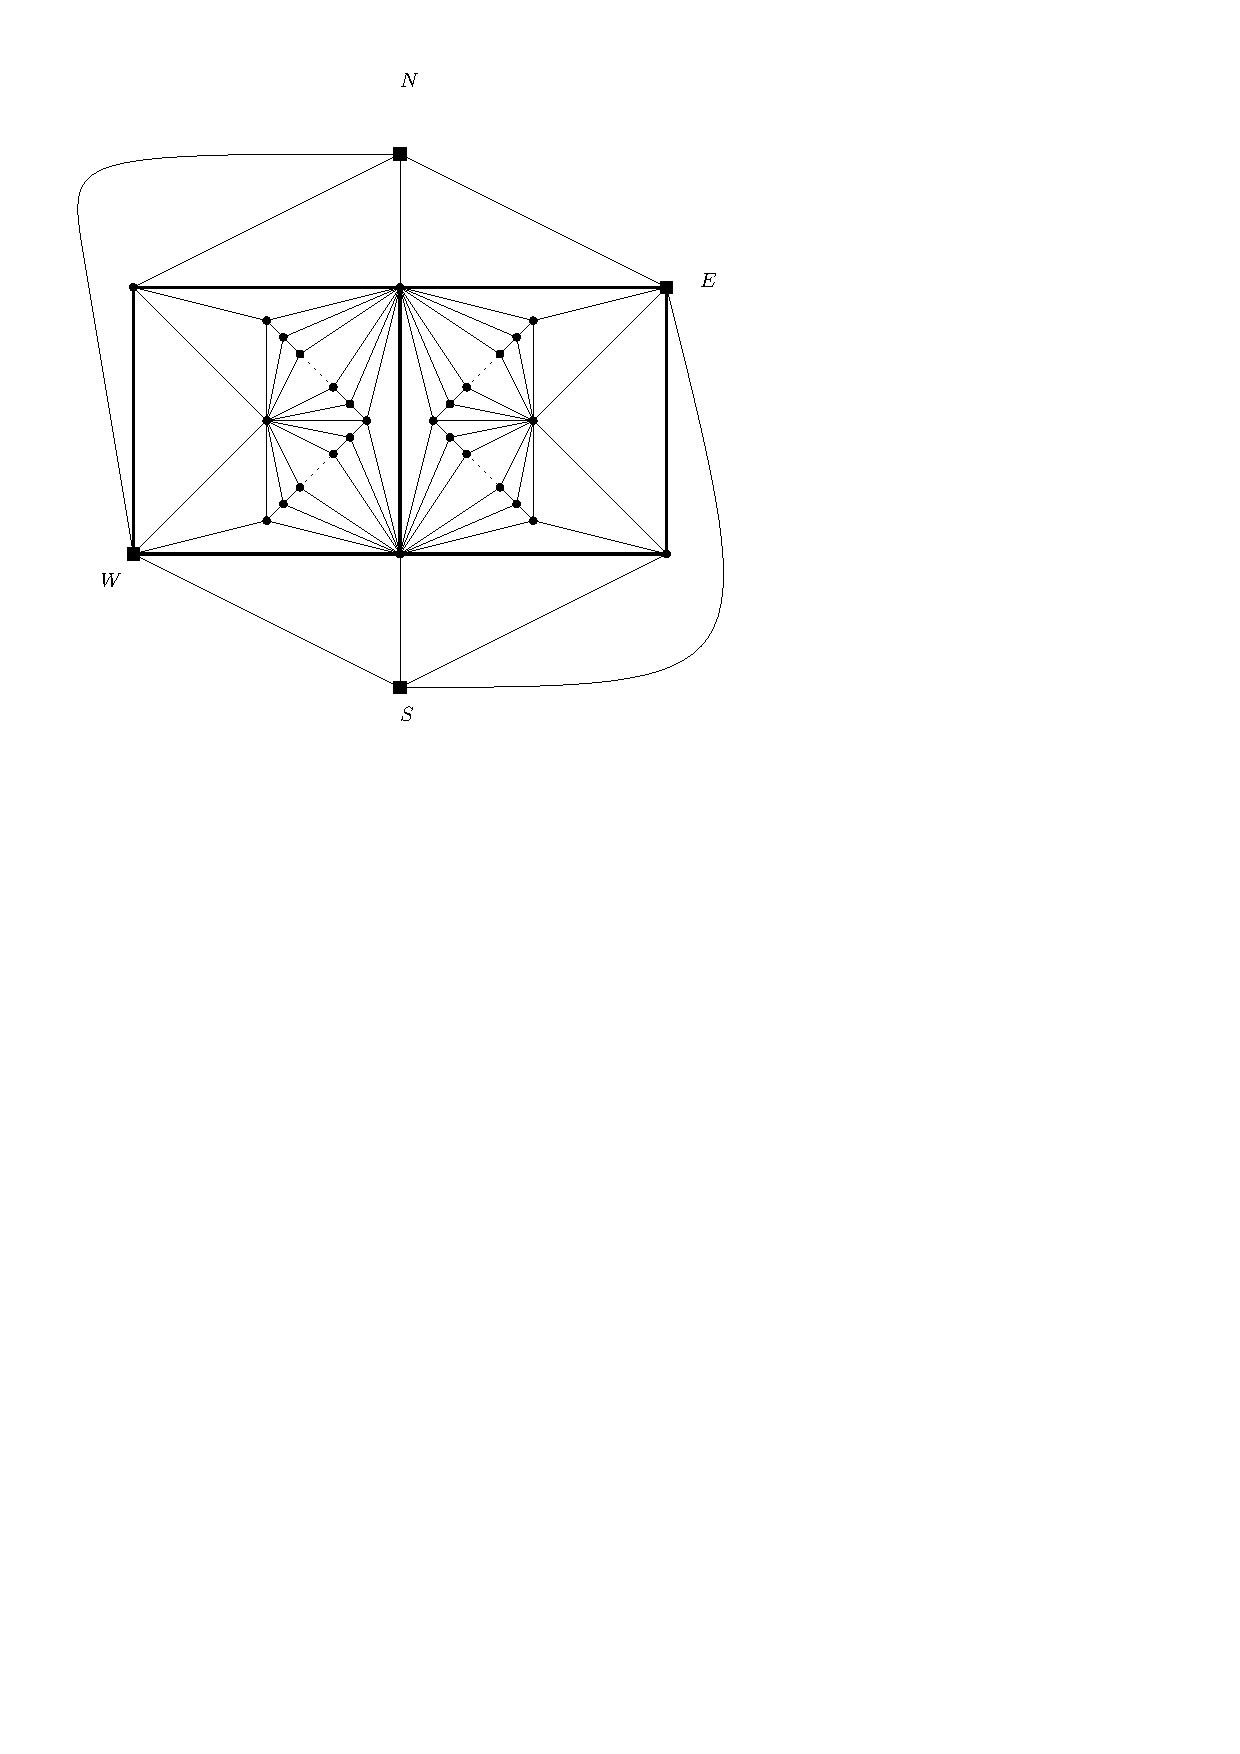
\includegraphics[scale=1]{fixExtension/img/manymanybase}
    \caption{A family of graphs not $k$-sided for any $k$}
    \label{fig:fix:manymany0}
  \end{figure}




  \begin{figure}[h]
    \centering
    \begin{subfigure}[t]{0.3\textwidth}
      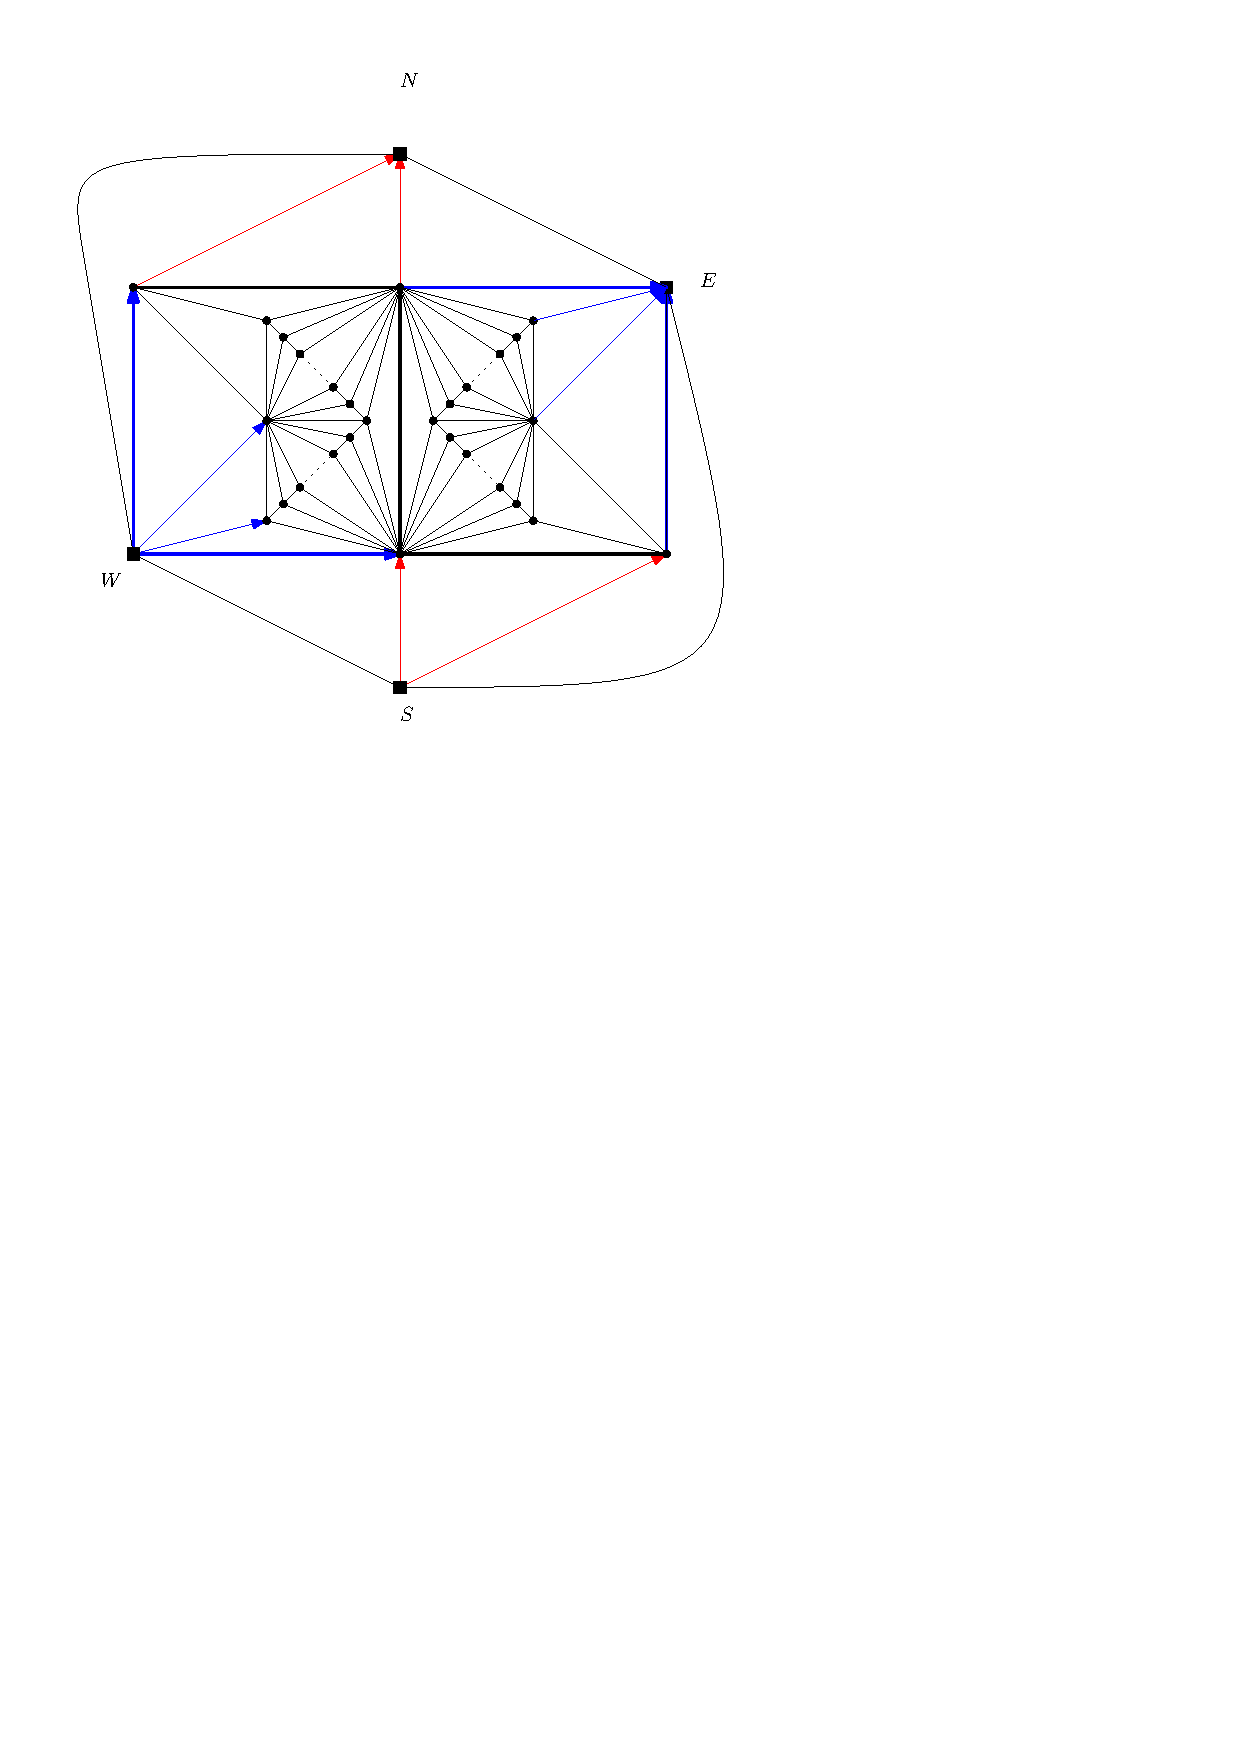
\includegraphics[width=\textwidth]{fixExtension/img/manymany1}
      \caption{Coloring the edges adjacent to the poles.}
      \label{fig:fix:manymany1}
    \end{subfigure}
    \quad
    \begin{subfigure}[t]{0.3\textwidth}
      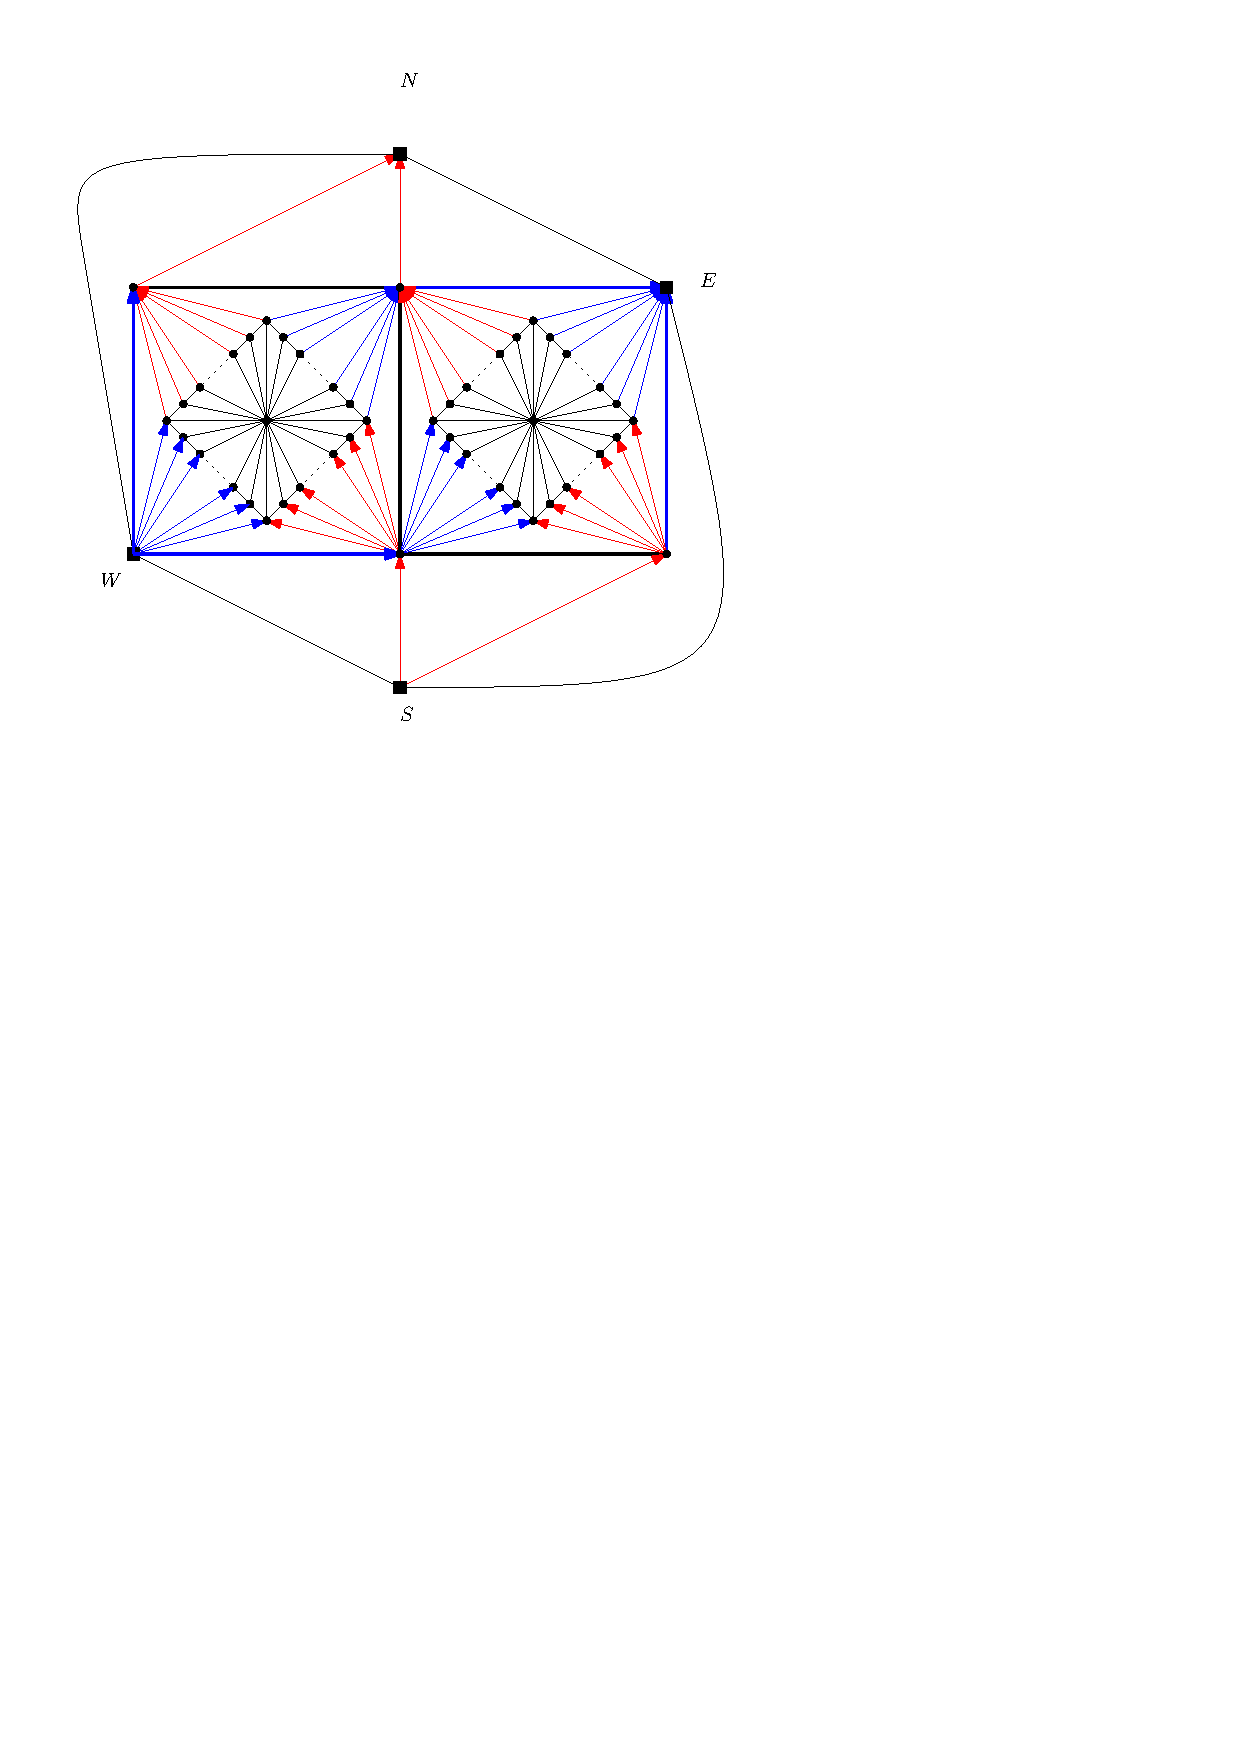
\includegraphics[width=\textwidth]{fixExtension/img/manymany2}
      \caption{Propagate trough the $4$-cycle.}
      \label{fig:fix:manymany2}
    \end{subfigure}
    \quad
    \begin{subfigure}[t]{0.3\textwidth}
      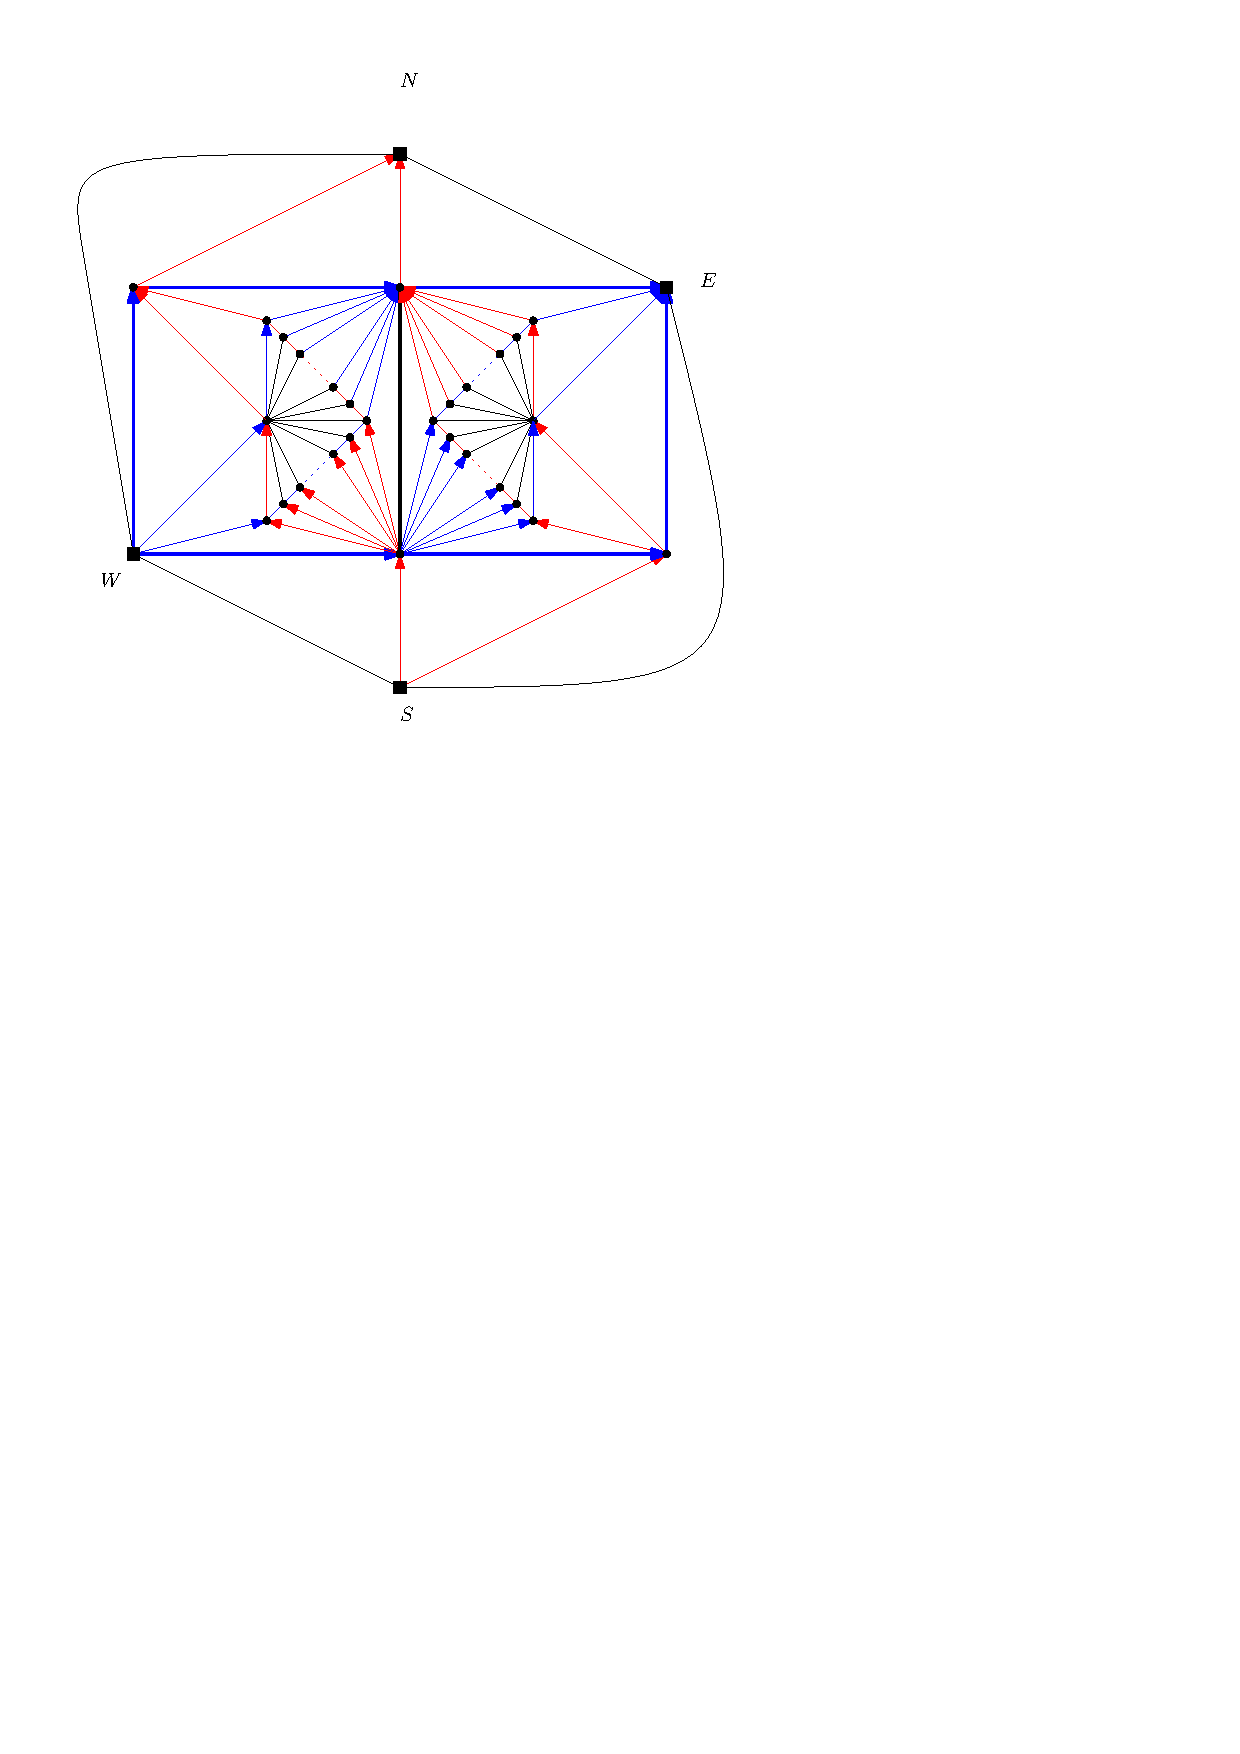
\includegraphics[width=\textwidth]{fixExtension/img/manymany3}
      \caption{Color such that there are no monochromatic triangles.}
      \label{fig:fix:manymany3}
    \end{subfigure}
    \caption{Coloring the graph.}
    \label{fig:fix:coloring}
  \end{figure}

  The result is then the graph displayed in Figure \ref{fig:fix:manymany4}. The black edges in this figure are edges that do not have a forced coloring by the above argument (Altough most of them can be forced by Lemma \ref{lm:fix:fourCycleInteriorColor}).
  We focus on the centered black edge $e$, $e$ is an interior edges of both the red and blue faces drawn with dashed edges in Figure \ref{fig:fix:manymany4}. Both boundary paths of these faces are of length larger than $k$. Hence, $e$ has to be colored both red and blue to prevent that face corresponding to a $k$-sided segment occurs in the regular edge labeling. An edge can not be colored red and blue at the same time and hence $G_k$ is not $k$-sided.

  Since this proof does not depend on the value of $k$, the family $G_k$ has graphs that are not $k$-sided for any $k$.
\end{proof}


  \begin{figure}[h]
    \centering
    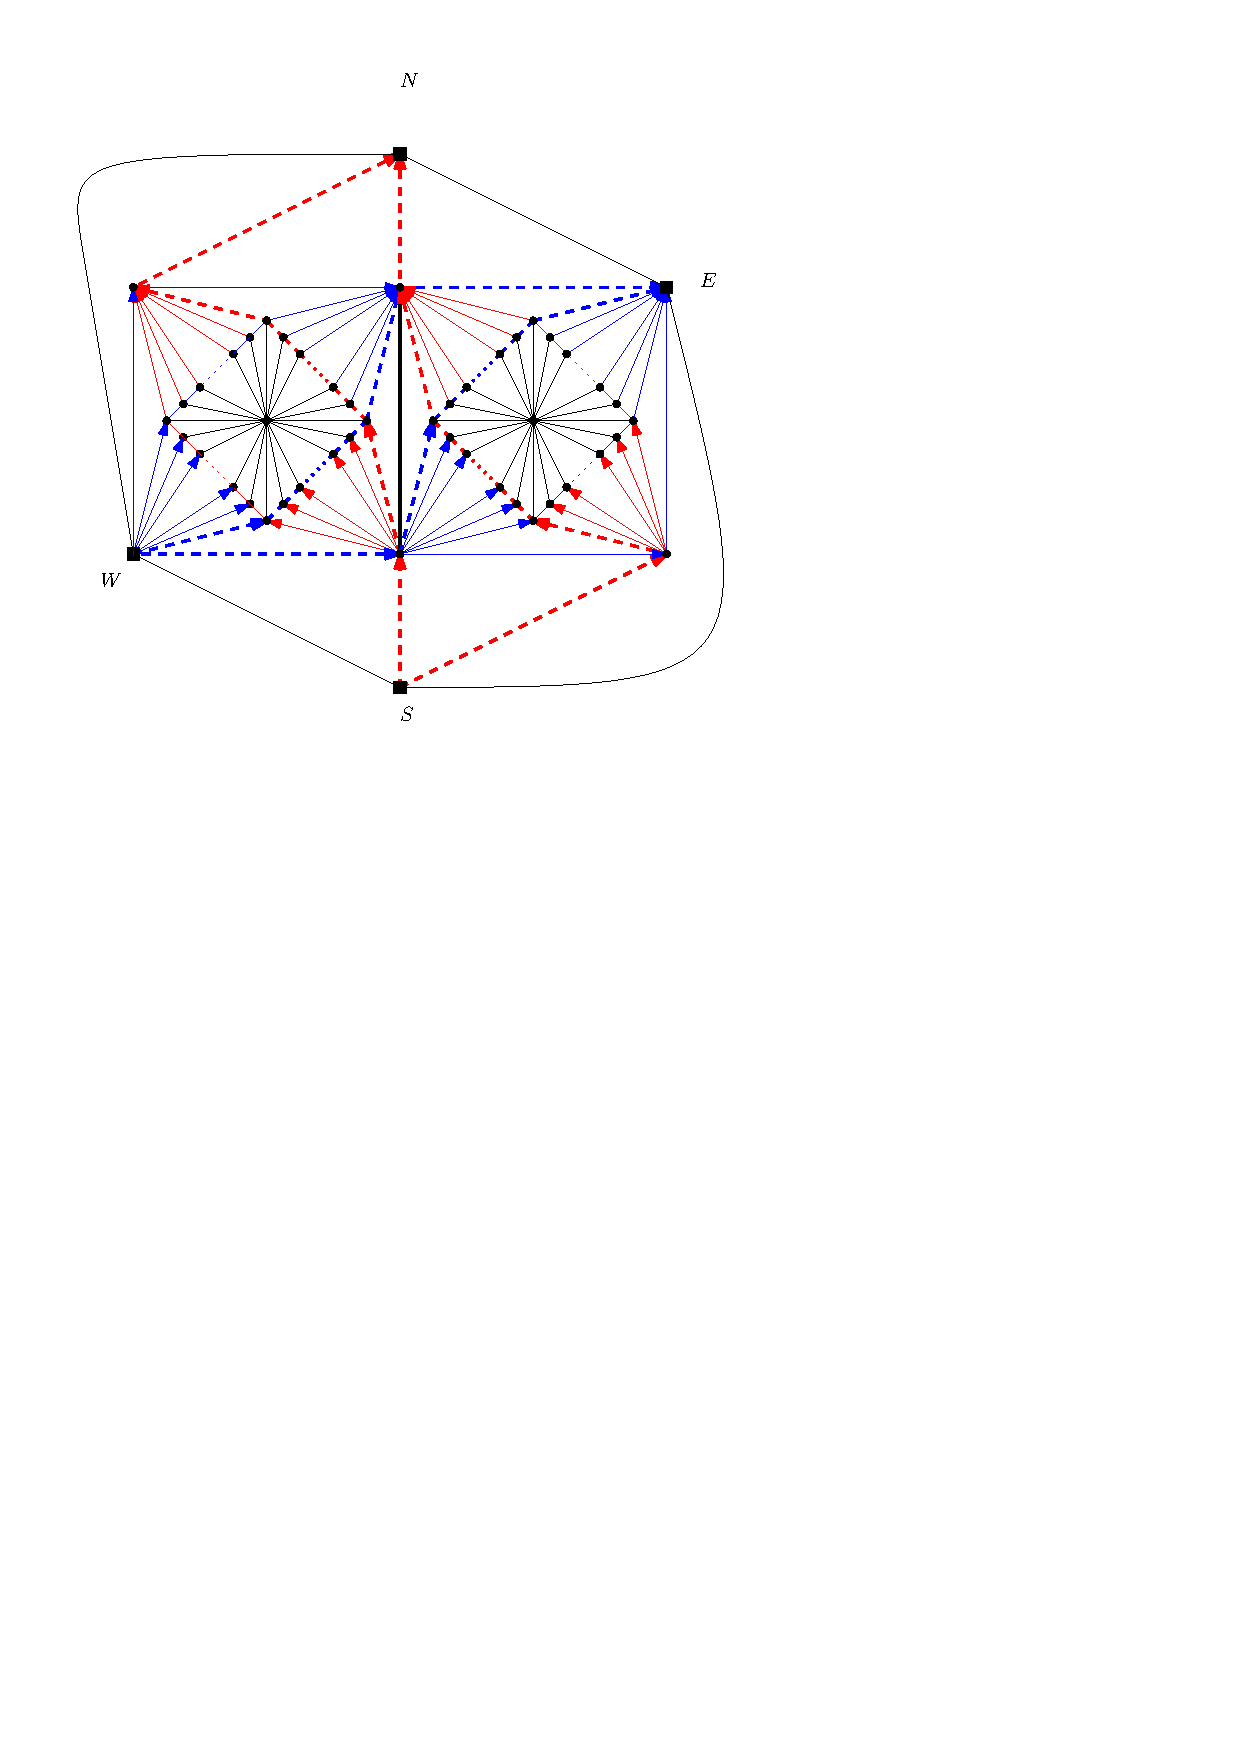
\includegraphics[scale=1]{fixExtension/img/manymany4}
    \caption{The graph after all coloring steps}
    \label{fig:fix:manymany4}
  \end{figure}


%!TEX root = ../thesis.tex

%invariant enviroment
\newenvironment{invariants}{%
  \refstepcounter{thrm}%
  \paragraph{Invariants~\theprop}%
  \renewcommand*{\theenumi}{\theprop\,(I\arabic{enumi})}%
  \renewcommand*{\labelenumi}{(I\arabic{enumi})}%
  \enumerate
}{%
  \endenumerate
}

\section{Algorithms}
\label{s:algo}
Kant and He \cite{Kant1997} were the first to design algorithms that determine a regular edge labeling.

Fusy \cite{Fusy2006} recently developed a different algorithm computing a specific regular edge labeling using a method shrinking a sweepcycle while coloring the outside in accordance with a regular edge labeling.\footnote{The specific regular edge labeling Fusy obtained was the minimal element of the distributive lattice of regular edge labellings.}

All algorithms in this section will have the same core (based on \cite{Fusy2006}). Consisting of shrinking a sweepcycle by so called \emph{valid} paths.\footnote{In Fusy's work he calls these \emph{eligible paths}} But will differ in which valid paths they choose (if there are multiple).

We will start this section with some notation and preliminaries in Subsection \ref{ss:not}. Then we will state the core algorithm and show that it always computes a regular edge labeling in Subsection \ref{ss:core}. Afterwards we show in Subsections \ref{ss:minimal}, \ref{ss:blue} and Section \ref{s:red} how one can adapt the choice of the valid paths to obtain regular edge labellings with certain properties. Namely a the minimal element of the distributive lattices of regular edge labellings and regular edge labeling corresponding to horizontal and vertical rectangular duals.


\subsection{Notation and Preliminaries}
\label{ss:not}
\begin{defi}[Interior path]
We call a path $P$ an internal path of a cycle $C$ if all vertices except the first and last one are in the interior of $C$ and it connects two distinct vertices of $C$
\end{defi}

We will use a script $\C$ to indicate the current sweep cycle.
We will repeatedly only consider the path $\cpath$. In that case we will always order it from $\pW$ to $\pE$. That these edges are always in $\C$ is a result of Invariant \ref{i:SWandSE}.

We will let $\P$ denote a interior path. Given such a path of $k$ vertices we will index it's nodes by $p_1, \ldots, p_k$ in such a way that $p_1$ is closer to $\pW$ then $p_k$ is (and thus that $p_k$ is closer to $\pE$ then $p_1$ is).

Then $p_1$ and $p_k$ indicate the two unique vertices of the walk that are also part of the cycle. We will then let $\restC{\P}$ denote the part of $\cpath$ that is between $p_1$ and $p_k$ (including). $\C_\P$ will denote the cycle we get when we paste $\restC{\P}$ and $\P$.



\subsection{Core}
\label{ss:core}

The algorithm will always maintain the following three invariants

\begin{invariants}
  \itemsep=-4pt

\item \label{i:SWandSE} The cycle $\C$ contains the two edges $\pS \pW$ and $\pS \pE$.
\item \label{i:noChords} $\cpath$ has no chords
\item \label{i:last} All inner edges of $T$ outside of $\C$ are colored and oriented in such that the inner vertex condition holds. %TODO what is the inner vertex condition
\fxerror{We need to add a partial inner vertex condition}
\end{invariants}

A cycle satisfying these three invariants will have the same general shape as in figure \ref{fig:invCycle}. We note that the cycle has at least $4$ vertices because otherwise a separating triangle is created.

\begin{figure}[h!]
\centering
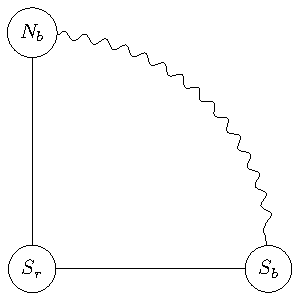
\includegraphics{algo/img/invCycle}

\caption{An example of a cycle $\C$ satisfying the invariants
    \label{fig:invCycle}}
\end{figure}

It is also nice to note that the union of the cycle and it's interior form a triangulation of the $n$-gon since it is a induced subgraph of a triangulation of the $4$-gon.


\subsubsection{Valid paths}

\begin{defi}[valid path]
We call an internal path $\P$ from $w_1$ to $w_k$ valid if
\begin{enumerate}
 \renewcommand*{\labelenumi}{(E\arabic{enumi})}%
 \renewcommand*{\theenumi}{(E\arabic{enumi})}%


\item Neither $p_1$ or $p_k$ is $\pS$
\label{e:noS}

\item The paths $\P$ and $\restC \P$ both have more than 1 edge \footnote{i.e. both have an interior vertex}
\label{e:longBorders}

\item Every interior edge of $\C_\P$ connects a vertex of $\P\setminus{\braces{p_1,p_k}}$ and $\restC \P \setminus{\braces{p_1,p_k}}$. In particular $\C_\P$ is a non-separating cycle.
\label{e:crossingEdges}

\item The path $\C'\sm{\pS}$, where $\C'$ is obtained by replacing $\restC \P$ by $\P$ in $\C$, is chordfree.
\label{e:noNewChord}

\end{enumerate}
\end{defi}

We note that \ref{e:crossingEdges} and \ref{e:noNewChord} partially overlap. \ref{e:crossingEdges} already implies that there can't be chords on the left of $\cpath$.


\begin{remark}
``Shrinking'' the cycle with an valid path will keep all the invariants true.
\end{remark}
\fxwarning[inline, nomargin]{We haven't proven this yet}

We will show the following proposition.



\begin{thrm}[Existence of a eligible path]
\label{th:eligExistence}
When the algorithm's invariant (\ref{i:SWandSE} - \ref{i:last}) are satisfied and the cycle $\C$ is separating then there exist a \emph{eligible} internal path.
\end{thrm}
\fxerror[inline, nomargin]{As outlined in last meeting this proof is not complete as is, it has been moved to the appendix. We are stuck on the part where we need to find a path satisfying E4. We might proof this from red algo.}



\subsection{Minimum distributive lattice element}
\label{ss:minimal}
We get this when we take the ``leftmost'' eligible path. As is outlined in \cite{Fusy2006}
\fxnote{Expand this subsection}

\renewcommand{\F}{\scr F}
\subsection{Horizontal one-sides}
\label{ss:blue}
\fxerror{Define what we mean with \emph{cycle border} and \emph{face border}}

As an exercise one could try to adapt Fusy's algorithm to generate horizontally one-sided layouts directly, without doing flips in the distributive lattice. It turns out that this is not that difficult.

Since the horizontal segments correspond to faces in the blue bipolar orientation we want that one of the two borders of the face has a length of at most two. Since every valid path which we update the cycle with splits off one face in the blue bipolar orientation it is easy to control this property.

\begin{thrm}
\label{th:blueelig}
In the update of the algorithm there is always an eligible path $\P$ available such that either $\P$ or $\restC{\P}$ is of length $2$.
\end{thrm}

In order to proof this theorem we will first show the following lemma.

\begin{lemma}
\label{lem:bluealgo}
If $\P$ is an eligible path giving raise to a cycle $\C_P$ of which both borders have length of at least $3$. Then there exist an eligible path $\P'$ such that the path border and cycle border of its cycle $\C_{\P'}$ are both at least $1$ shorter than those of $\C_\P$.
\end{lemma}

\fxnote{Revisit notation after writing section on oriented REL}
\begin{proof}
In this proof we will frequently use property \ref{e:crossingEdges} of a valid path, we won't mention it every time we use it.

We denote the source by $s$ and the sink by $t$. We also assign names$a, b$ and $x, y$ to the first two vertices on both borders, see Figure \ref{fig:bluealgo:notation}. Since every interior face of $G$ is a triangle $ax$ is an edge. Now we distinguish two cases, either $ay$ is an edge (case 1) or $bx$ is an edge (case 2). They can't both be an edge at the same time due to planarity, neither can it happen that both of them are not an edge since then the face containing the path $baxy$ is at least of degree $4$.

In the first case $a$ may be connected to more vertices on the path border, however there is a last one, say $z$. And this vertex is then also connected to $b$, otherwise it would not be the last one. Now we can provide an shorter eligible path $\P'$. We start at $a$ go to $z$ and from there we follow the old path $\P$ to $t$.  See figure \ref{fig:bluealgo:case1}. It is easy to see that all four properties of an eligible path hold for $\P'$.
\begin{comment}
By construction $\P'$ satisfies \ref{e:noS} and \ref{e:internalVertices}. While the interior of $\C_{\P'}$ is a subset of that $\C_\P$%TODO this is again an eligible path
\end{comment}

In the second case $x$ may be connected to more vertices along the cycle border, however there is a last one, say $c$. And this vertex is then also connected to $y$, otherwise it would not be the last one. Now we can provide an shorter eligible path $\P' = sxz$.   See figure \ref{fig:bluealgo:case2}. It is straightforward to see that all four properties of an eligible path hold for $\P'$. %TODO this is again an eligible path
\end{proof}

\begin{figure}[ht]
    \centering
    \begin{subfigure}[b]{0.45\textwidth}
        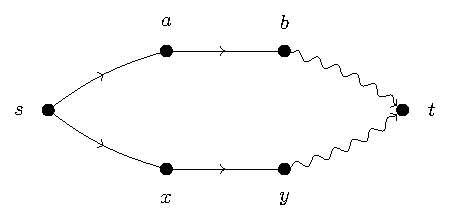
\includegraphics[width=\textwidth]{algo/img/blue/setting}
        \caption{The setting}
        \label{fig:bluealgo:notation}
    \end{subfigure}

    \begin{subfigure}[b]{0.45\textwidth}
        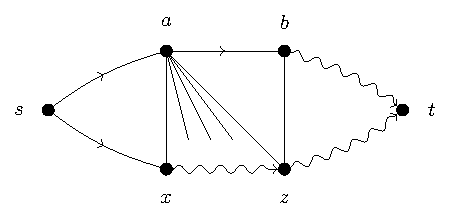
\includegraphics[width=\textwidth]{algo/img/blue/case1}
        \caption{Case 1}
        \label{fig:bluealgo:case1}
    \end{subfigure}
    ~
    \begin{subfigure}[b]{0.45\textwidth}
        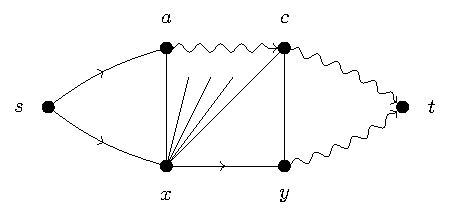
\includegraphics[width=\textwidth]{algo/img/blue/case2}
        \caption{Case 2}
        \label{fig:bluealgo:case2}
    \end{subfigure}

    	\caption{}
\end{figure}

\begin{proof}[Proof of Theorem \ref{th:blueelig}]
By Theorem \ref{th:eligExistence} we know there is a eligible path $\P$. If one of the borders of $\C_\P$ is of length $2$ or less we are done. If this path gives raise to a face $\C_\P$ with both borders are both of length at least $3$ we can repeatedly apply Lemma \ref{lem:bluealgo} until at least one of the borders is of length at most $2$.
\end{proof}

If we in every update of the algorithm take the paths from Theorem  \ref{th:blueelig} we end up with the correct faces in the blue bipolar orientation and hence a horizontally one sided rectangular dual.


%!TEX root = ../thesis.tex

\section{The right neighbor path of a path}
\thispagestyle{plain}
  \label{s:rightNeighbour}
  In the sweepcycle step of the algorithm (Section \ref{s:sweep}) we will use the \emph{right neighbor path} of a path. In this section we show that for any path $P = p_1 \ldots p_k$ with no interior vertices incident to the outer face and without chords or separating 2-chords on the right of the path, the right side neighbors of $P$ are a path (Lemma \ref{lm:uni:neighborPath}).
  We even show some additional properties hold for this path $P$.
  Similar things also hold for the the left neighbors of $P$ but we will not need this for the proof of our algorithm.

  The right side of a path is not yet defined and to do this we introduce the notion of rotations at a vertex. During the proofs in this section we will also need various types of chords so we subsequently introduce these.

  \mypar{Rotations}
    We assume a fixed embedding for $G$. The \emph{rotation} at a vertex $v$ is the clockwise order of the edges incident to $v$. We will identify these edges with their other endpoints.
    Two vertices $x, y$ are said to be \emph{consecutive} in the rotation at $v$ when the edges $vx$ and $vy$ are consecutive in the rotation.
    We sometimes want to denote number of subsequent vertices, which we call an \emph{interval}, in the rotation. We let $[x,y]$ denote all the vertices in the rotation of $v$ from $x$ to $y$ and we let the \emph{exclusive interval} $(x,y)$ denote the same vertices without $x$ and $y$.

    Given a path $P$ and a interior vertex $p_i \in P$. A neighbor $v \nin \P$ of $p_i$ lies on the \emph{left} of $P$ if it lies in the interval $(p_{i-1}, p_{i+1})$ in the rotation of $p_{i}$. Otherwise $v$ lies in the interval $(p_{i+1}, p_{i-1})$ in the rotation of $p_i$. In this case $v$ lies on the \emph{right} of $P$.
    We will use the same notion of left and right for edges. That is, an edge $e\nin P$ adjacent to $p_i$ lies to left or right if its other end point lies to the left or right, respectively. In Figure \ref{fig:right:rot} $v$ and $p_i v$ lie on the left of $P$ and $u$ and $p_i u$ lie on the right of $P$.

    \begin{figure}[h]
      \centering
      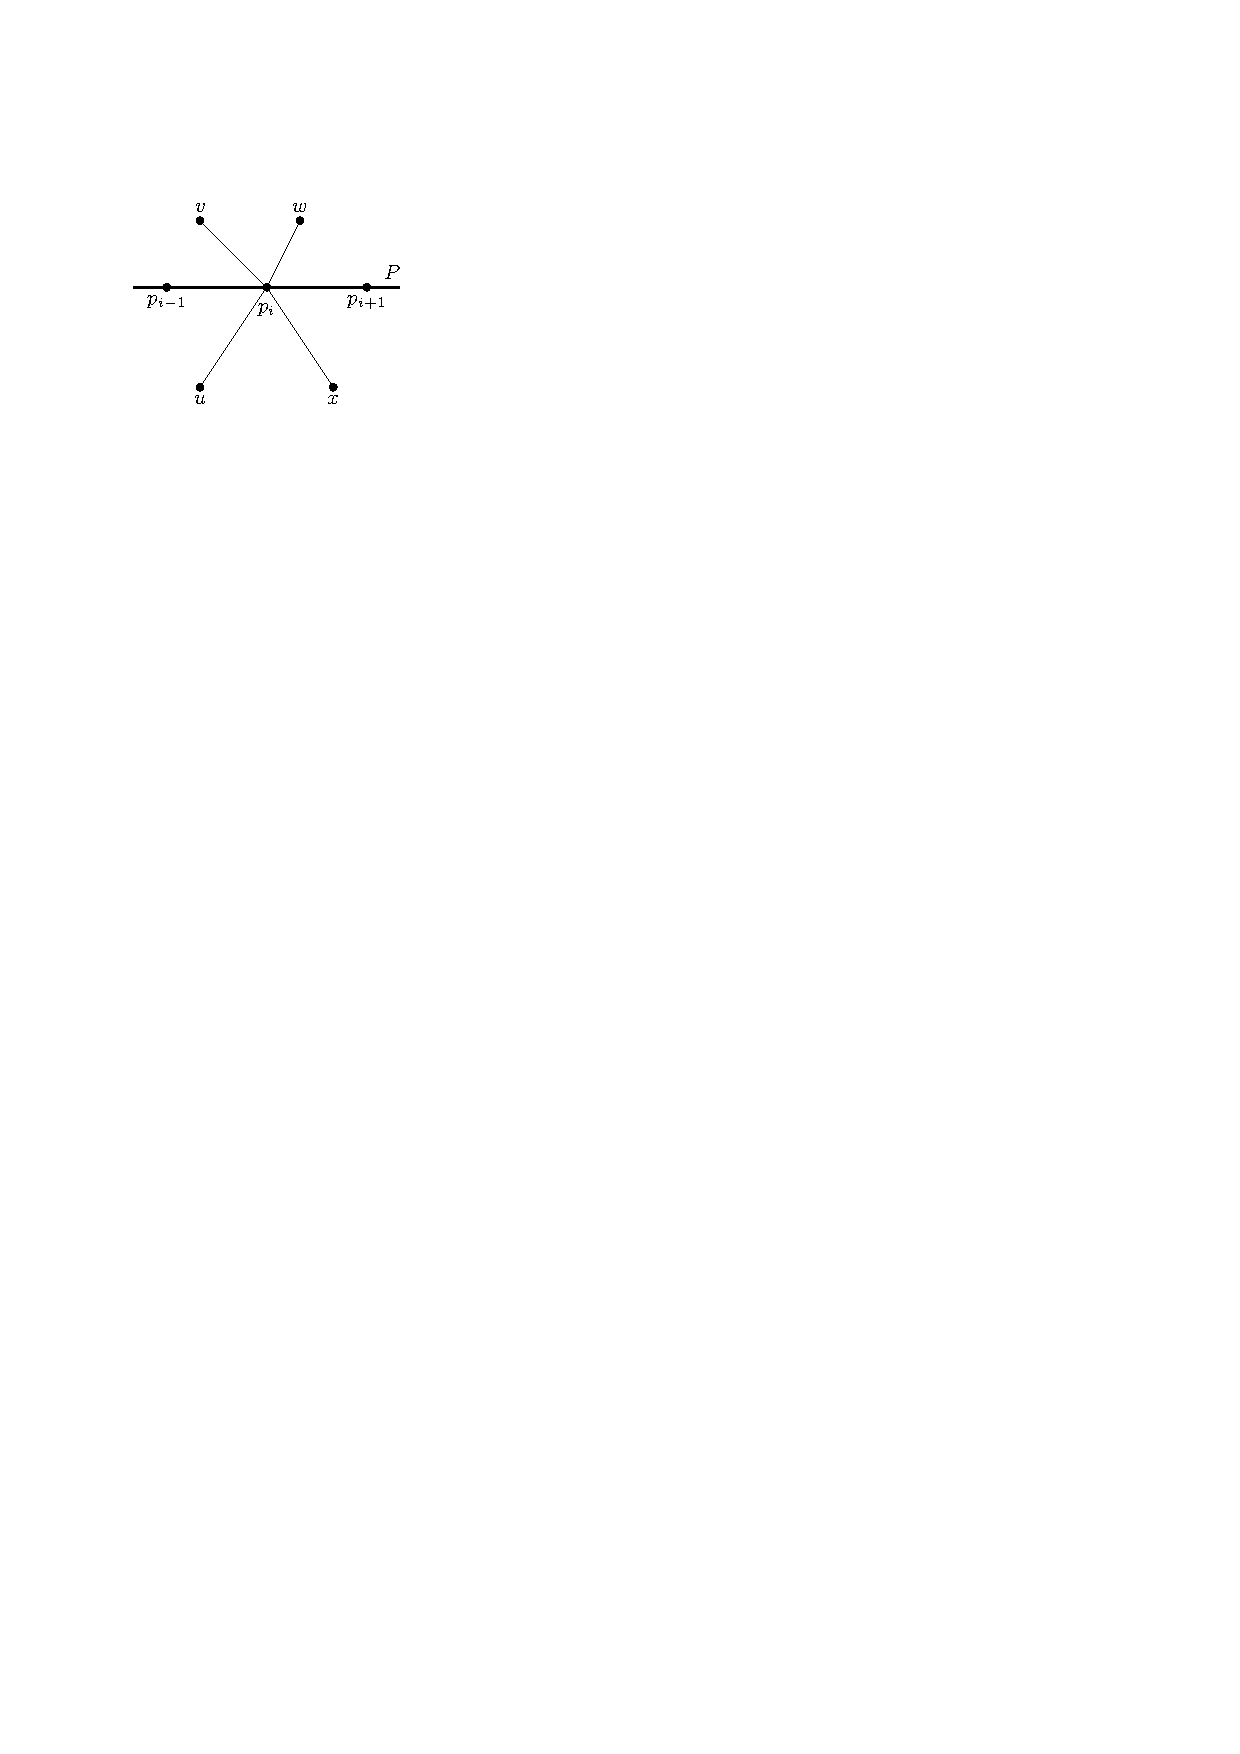
\includegraphics[scale=1]{unifiedAlgo/img/rightNeighbourwalk/rotation}
      \caption{}
      \label{fig:right:rot}
    \end{figure}

  \mypar{Path manipulations}
    With $\rev{P}$ we denote the \emph{reversed path} $p_k \ldots p_1$. We use $\oplus$ to denote the \emph{concatenation} of paths. That is, given a second path $\Q$ with vertices $q_1 \ldots q_l$ and $p_k = q_1$ the path $\P \oplus \Q$ consists of $p_1 \ldots p_{k-1} q_1 q_2 \ldots q_l$.
    Recall that a cycle is simply a path starting and ending at the same vertex. Hence if we have two  internally disjoint paths $\P, \Q$ from $s$ to $t$ then $\P \oplus \rev{\Q}$ is a cycle.
    Furthermore we use a vertical bar to denote the \emph{restriction} of a path to a certain set of vertices. So $\P|_{p_i, p_j}$ with $i<j$ is the subpath of $\P$ with vertices $p_i \ldots p_j$.

  \mypar{Chords}
    A \emph{chord} of a path is an edge that connects two non-subsequent vertices. A path without chords is \emph{chordfree}. The path $P$ in Figure \ref{fig:right:chord} has the chord $p_1 p_3$.
    A \emph{k-chord} is a path $Q$ of length $k$ that connects two non-subsequent vertices $p_i, p_j$ of $P$ such that $P \cap Q = \braces{p_i, p_j}$.
    Note that $\P|_{v_i, v_j} \oplus \rev{\Q}$ is a cycle.
    A ($k$-)chord $Q$ is \emph{separating} if this cycle is separating. In Figure \ref{fig:right:chord} there are two $2$-chords, $p_3 u p_5$ and $p_3 v p_5$, but only one of them is separating, namely $p_3 v p_5$.
    Since a cycle is a special type of path the same definitions apply to them.

  \begin{figure}[h]
    \centering
    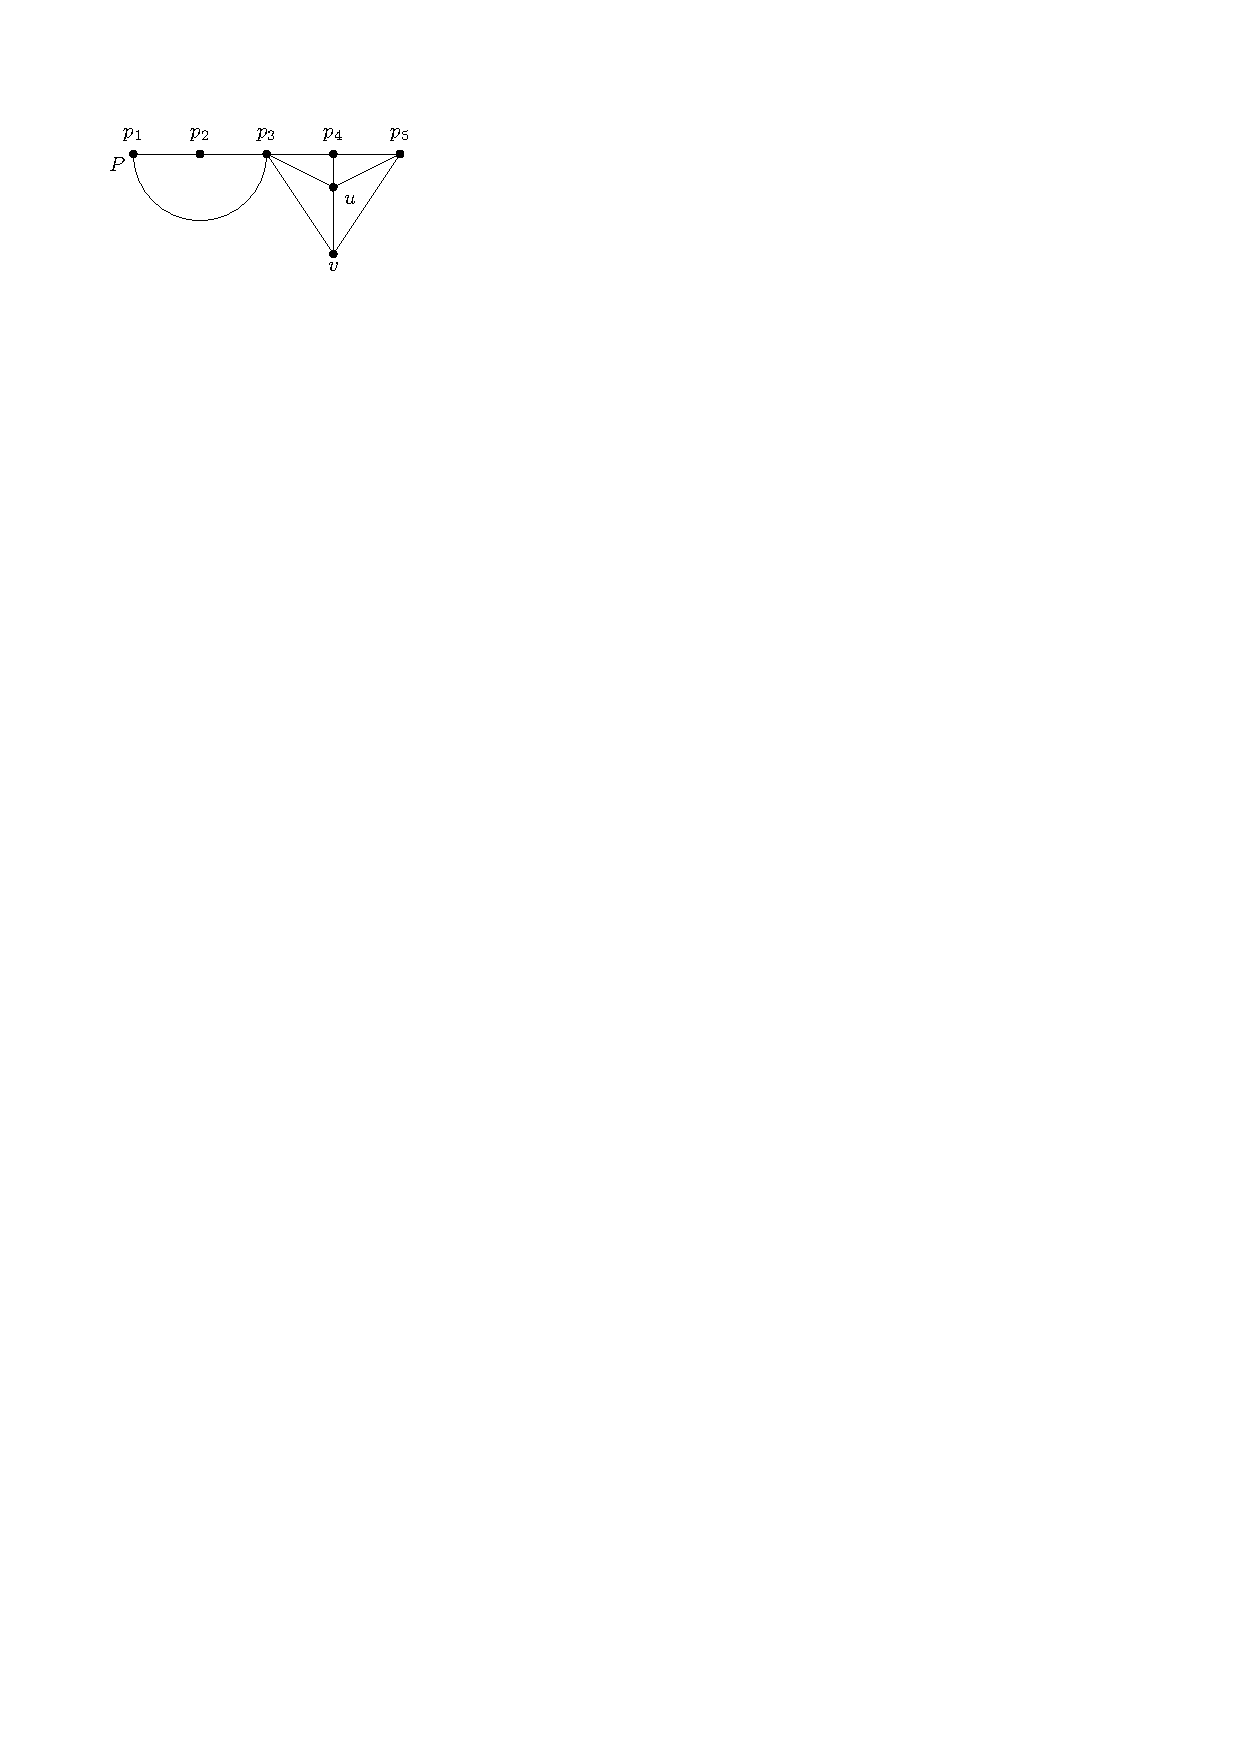
\includegraphics[scale=1]{unifiedAlgo/img/rightNeighbourwalk/chords.pdf}
    \caption{A path with a chord and a separating 2-chord}
    \label{fig:right:chord}
  \end{figure}

  \mypar{Right neighbor paths}
    We already mentioned that in the sweepcycle step we use the right neighbor path of a path. Recall that  $P$ has no interior vertices incident to the outer face and no chords or separating 2-chords on the right. We first show that every vertex has right neighbours, then we give the procedure for making the right neighbor path. Afterwards we show that the right neighbour path is a walk (Lemma \ref{lm:uni:neighborWalk}) and a path (Lemma \ref{lm:uni:neighborPath}).

    \begin{lemma}
      \label{lm:right:pHasRightNeihgbours}
      Every interior vertex of $P$ has at least one neighboring vertex on the right.
    \end{lemma}

    \begin{proof}
      Suppose that a interior vertex $p_i$ has no neighbor on the right of the path. Then $ \ldots p_{i-1} p_i p_{i+1} \ldots $ is a partial face border. Since $p_i$ is not incident to the outer face $p_i$ must be incident to a face of degree $3$. Thus $p_{i-1} p_i p_{i+1}$ is a face. However, this would imply a chord on the right of $P$ as can be seen in Figure \ref{fig:right:pHasRightNeighbor}. Hence by contradiction $p_i$ must have a neighbor on the right.
    \end{proof}

    \begin{figure}[h]
      \centering
      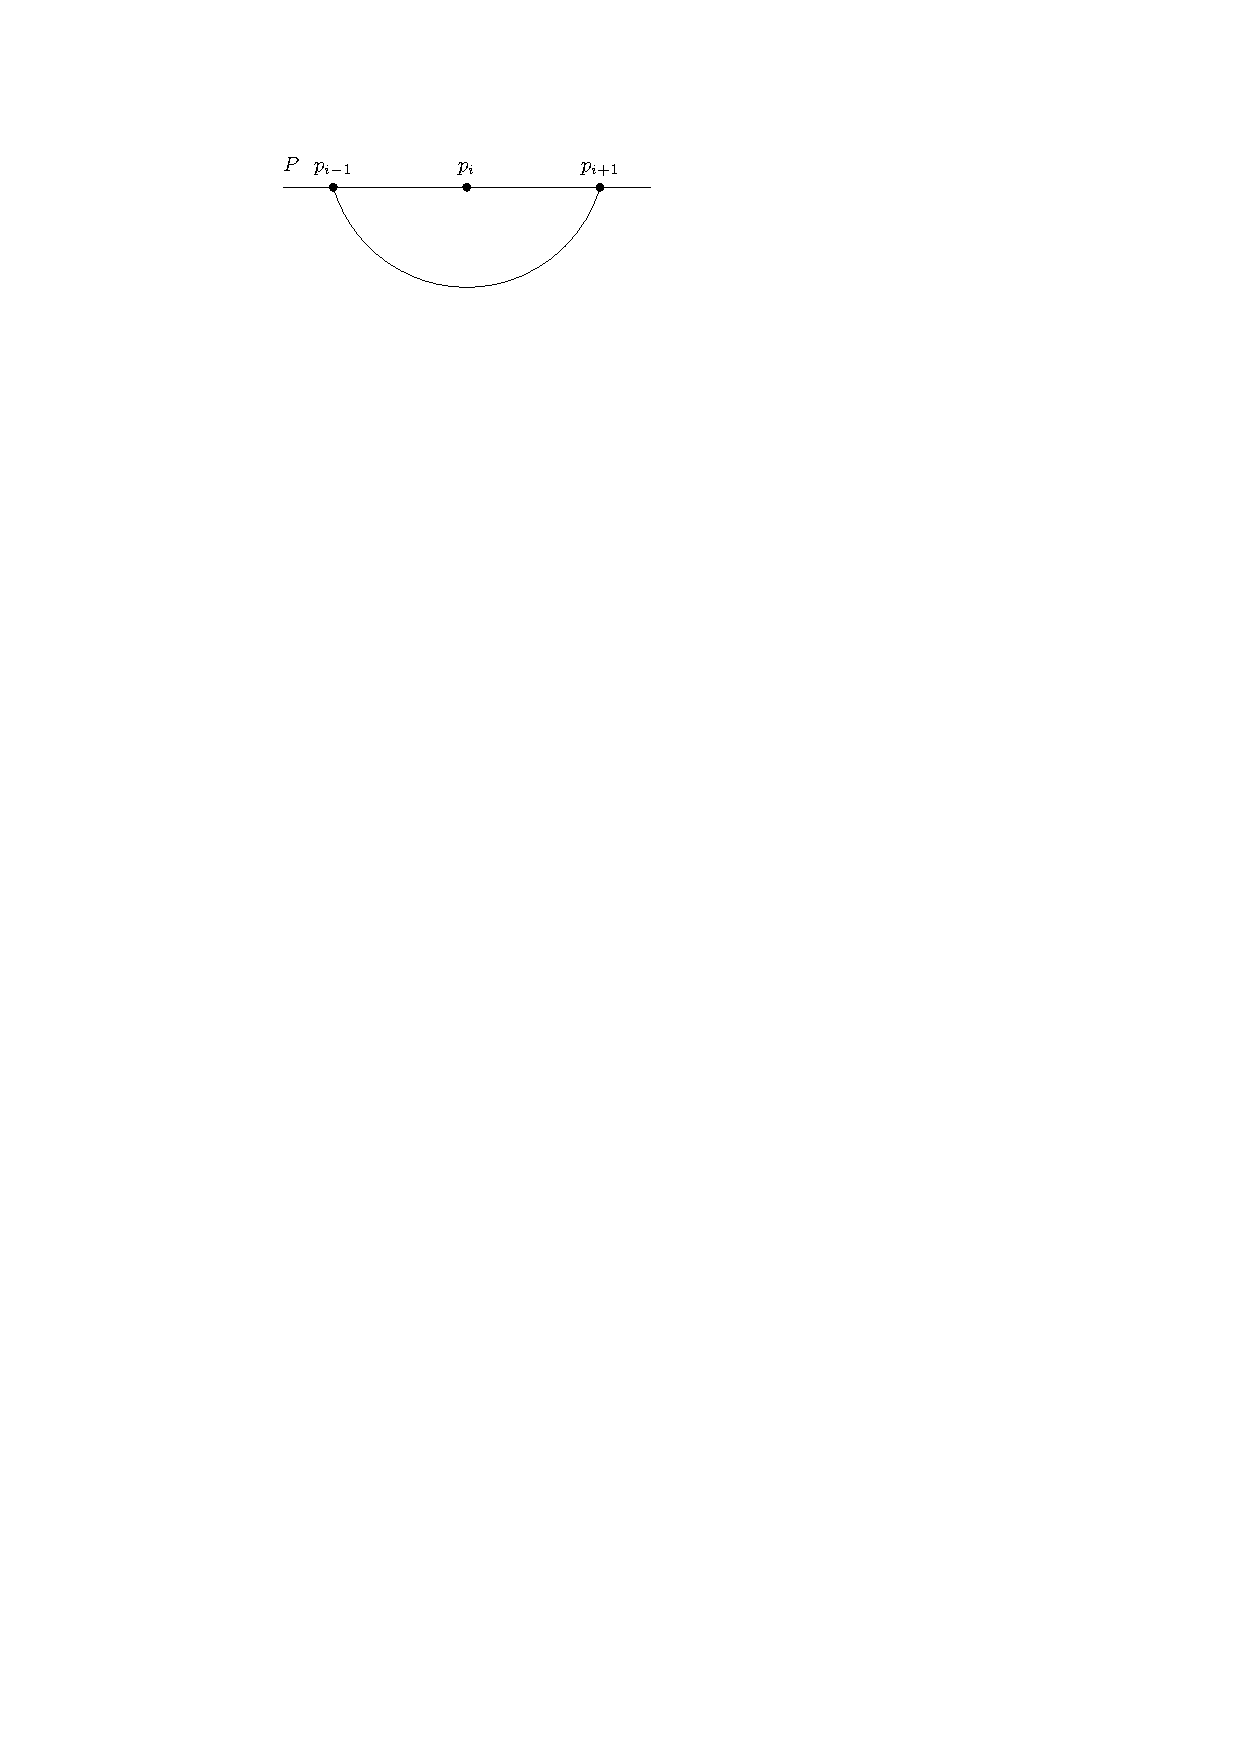
\includegraphics[scale=1]{unifiedAlgo/img/rightNeighbourwalk/pHasRightNeighbor.pdf}
      \caption{}
      \label{fig:right:pHasRightNeighbor}
    \end{figure}

    These right neighbors of $P$ will form the the \emph{right neighbor path} $Q$ of $P$.
    Let us first define a larger list of vertices $Q'$. $Q'$ will consist of $p_1$ and those vertices adjacent to $p_{2}$ that are in the exclusive interval $(p_1, p_3)$ of the clockwise rotation at $p_2$. Followed by the vertices in the interval $(p_2, p_4)$ of the rotation at $p_{3}$. We continue this up to the vertices in the interval $(p_{k-2}, p_k)$ of the rotation at $p_{k-1}$ and finally $p_k$.
    We obtain $Q$ from $Q'$ by removing all subsequent duplicates from $Q$.
    In Figure \ref{fig:right:neighborPath} an example of a right neighbor path is given.

    \begin{figure}[h]
      \centering
      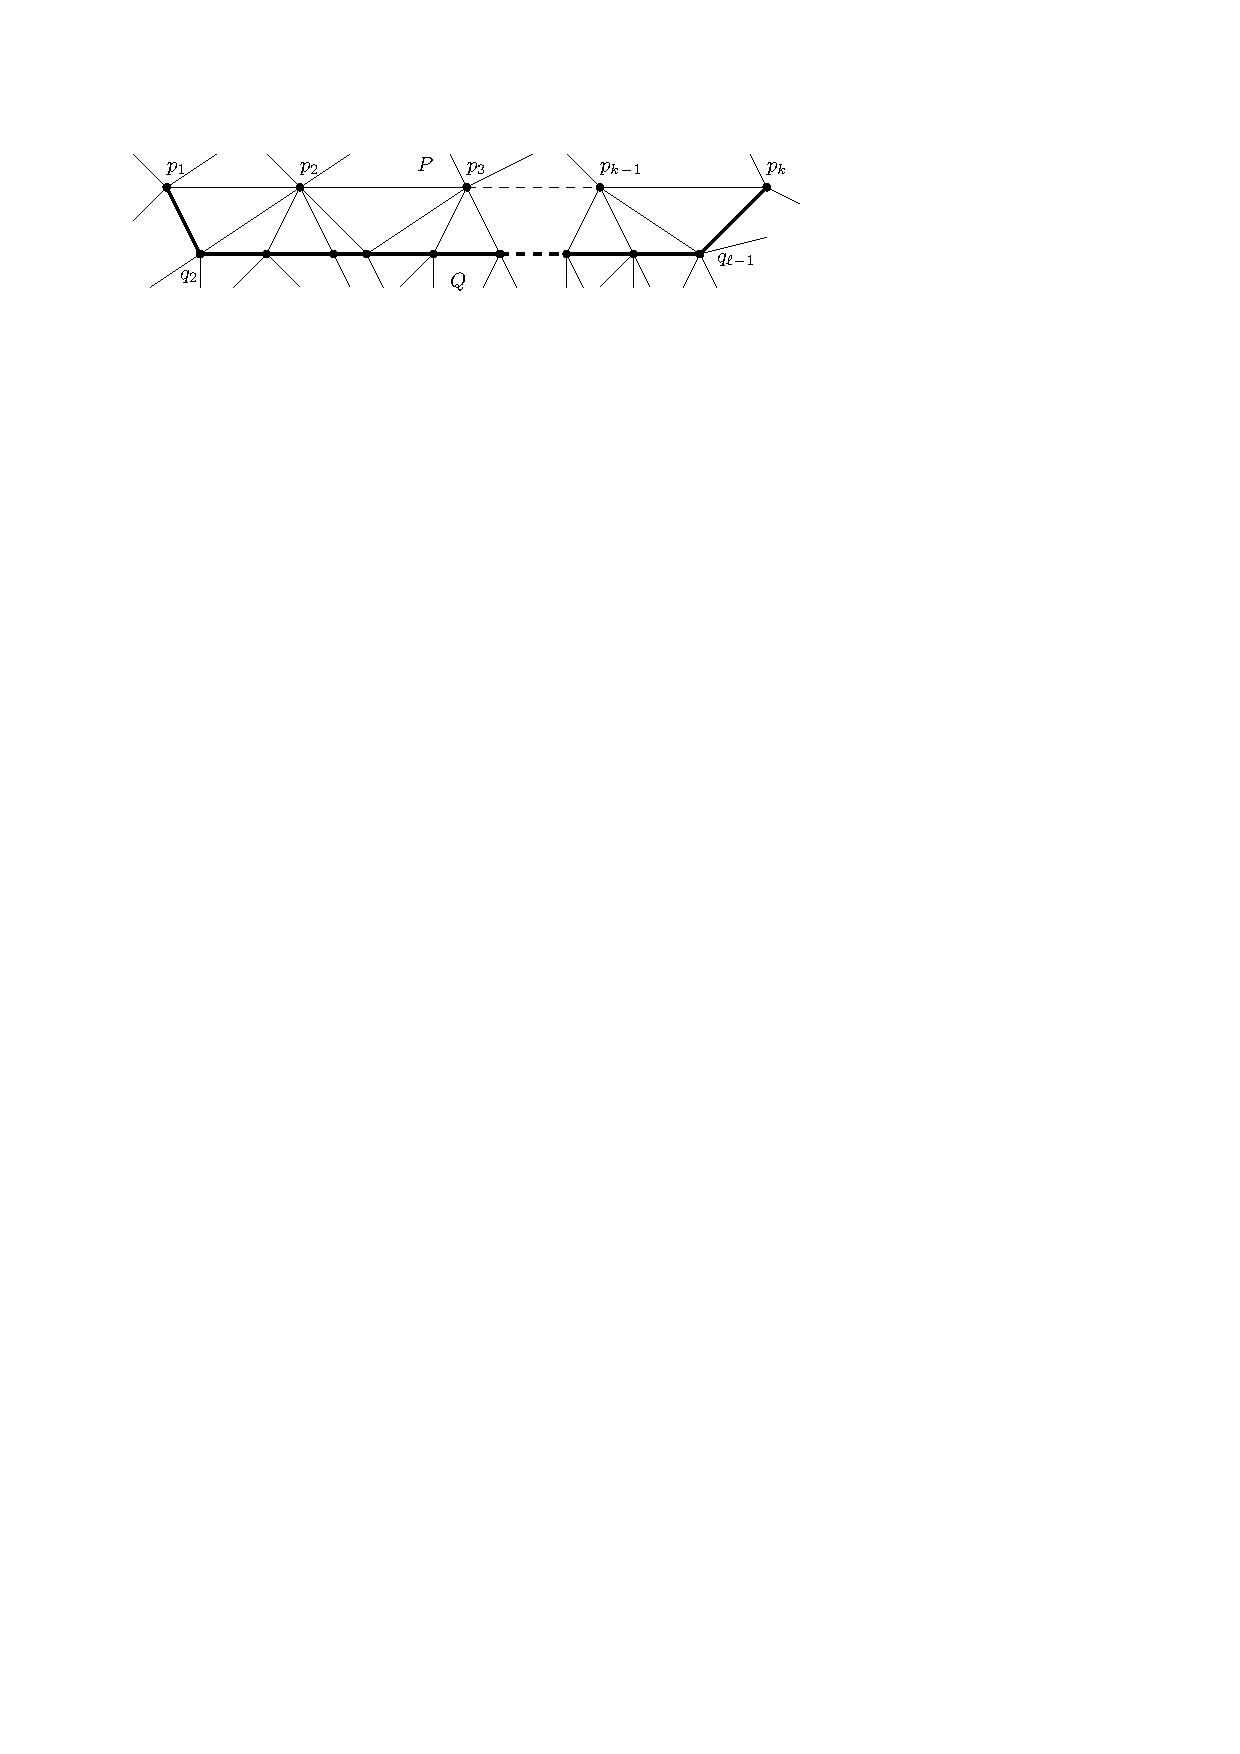
\includegraphics[scale=1]{unifiedAlgo/img/rightNeighbourwalk/neighborPath.pdf}
      \caption{}
      \label{fig:right:neighborPath}
    \end{figure}


  To break the proof that $Q$ is a path into two parts we define a \emph{walk} as a path without the constraint to be simple. Hence a walk is a sequence of vertices that are connected to each other but vertices may repeatedly occur.
  \begin{lemma}
    \label{lm:uni:neighborWalk}
    The right neighbor path $Q$ is a walk.
  \end{lemma}
  \begin{proof}
    Let us denote the vertices of $Q$ by $q_1 q_2 \ldots q_\ell$.
    Let $q_i$ and $q_{i+1}$ be two subsequent vertices of $Q'$. We will show they are either connected or the same vertex. We first consider the case where $1 < i < \ell-1$.
    Now there are two sub-cases. Either $(a)$ $q_i$ and $ q_{i+1}$ are vertices adjacent to the same vertex $p_j$ an thus subsequent in the rotation at $p_j$ or $(b)$ $q_i$ was the last vertex adjacent to $p_j$ and thus $q_{i+1}$ is the first vertex adjacent to $p_{j+1}$ since by Lemma \ref{lm:right:pHasRightNeihgbours} every interior vertex of $P$ has right neighbors.
    Both cases are depicted in Figure \ref{fig:uni:walkproof}

    In case $(a)$ we note that since $q_i$ and $q_{i+1}$ are subsequent in the rotation at $p_j$ $q_i q_{i+1}$ is an edge since $p_j$ is not incident to the outer face and every interior face of $G$ is a triangle.

    In case $(b)$ we note that $p_i q_i$ and $p_i p_{i+1}$ are edges subsequent in clockwise order, hence $q_{i} p_{i+1}$ is also an edge. Hence $q_i$ is the first vertex adjacent to $p_{i+1}$ subsequent to $v_i$ in the clockwise rotation. Thus $q_{i} = q_{i+1}$. They are duplicates.

    Now for the cases $i=1$ and $i=k-1$. $q_1$ and $q_2$ are vertices adjacent to $p_{2}$ subsequent in the clockwise rotation of ${p_2}$ and hence connected since every interior face is a triangle. In the same way $q_{k-1}$ and $q_k$ are subsequent vertices in the rotation at $q_{k-1}$ and hence connected. This can also be seen in Figure \ref{fig:right:neighborPath}.

    Since all pairs of subsequent vertices in $Q'$ are connected or duplicates the step removing all duplicates from $Q'$ ensures $Q$ is a walk.

    \begin{figure}[b]
      \centering
      \begin{subfigure}[b]{0.5\linewidth}
          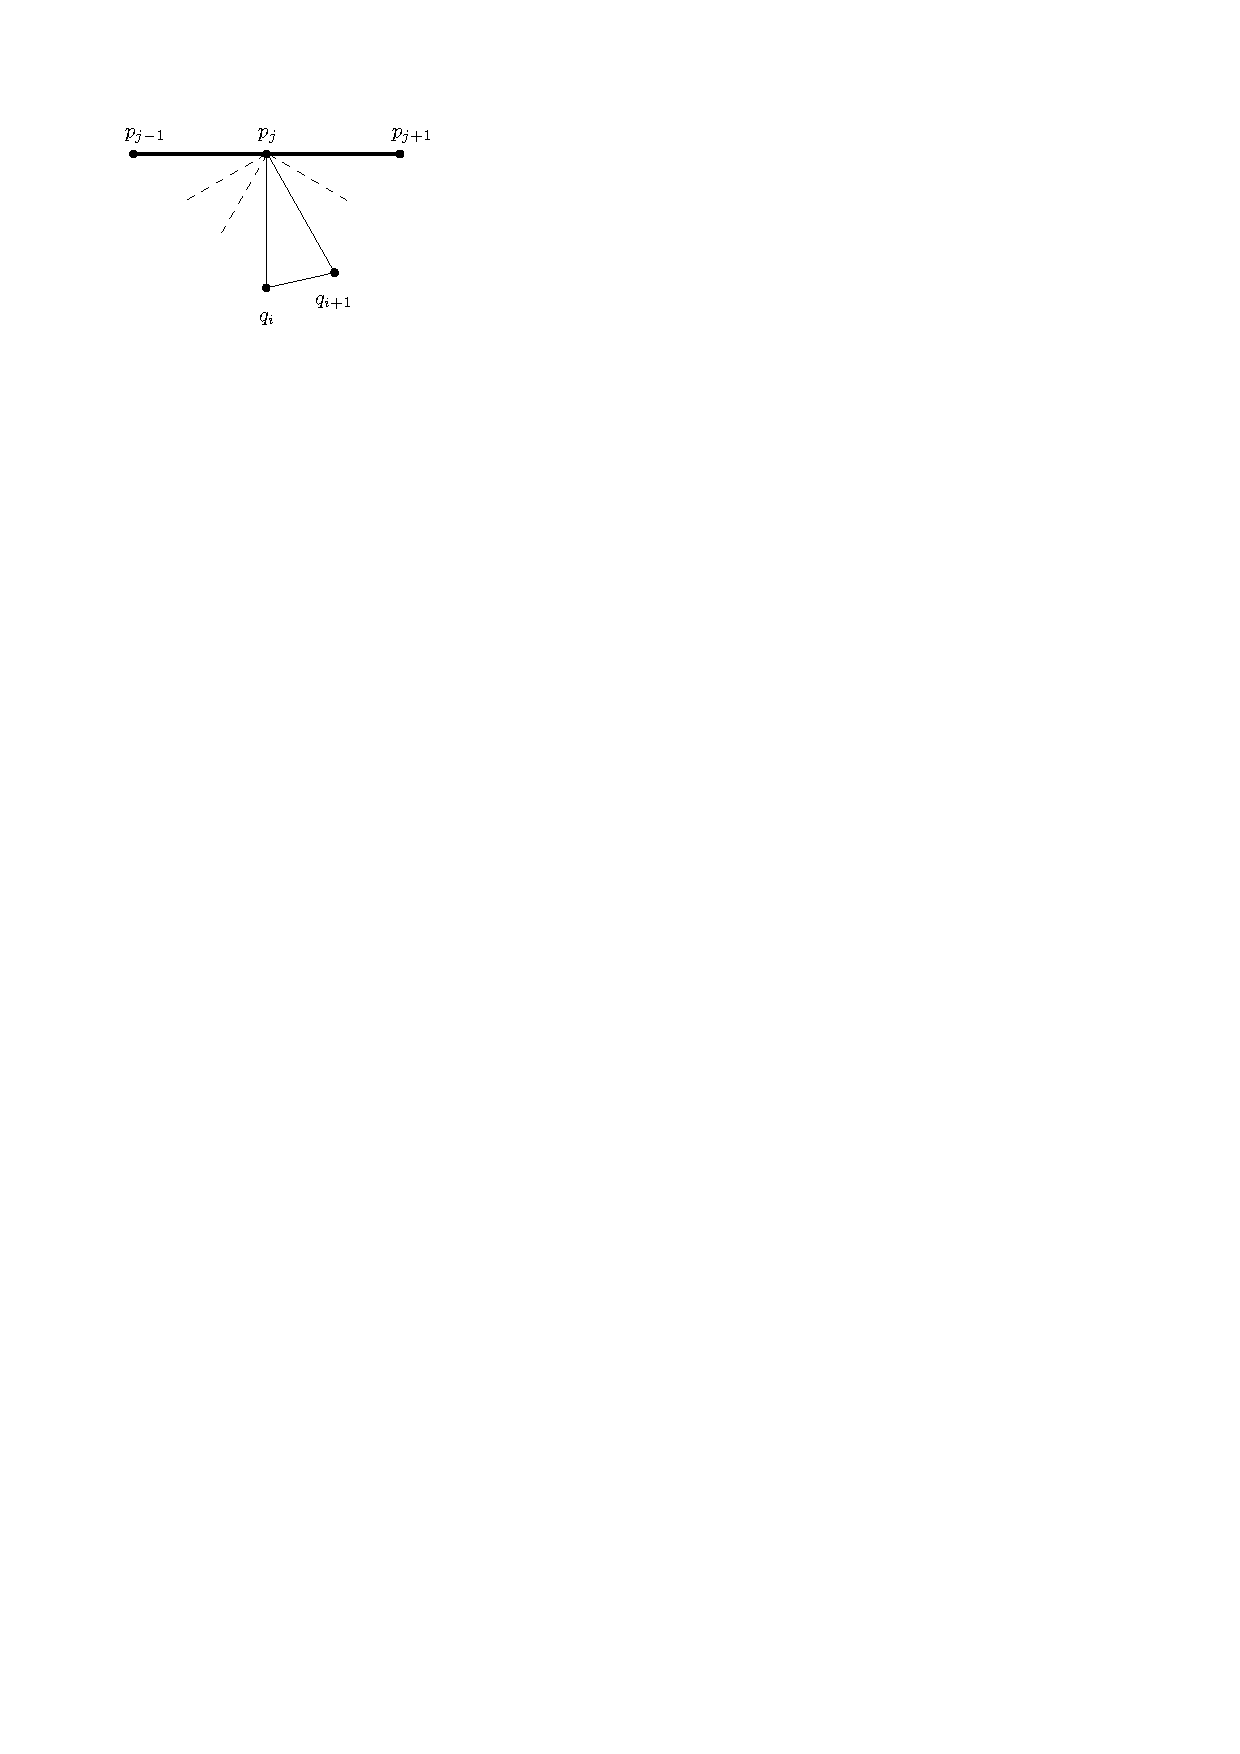
\includegraphics[width=\linewidth]{unifiedAlgo/img/walkProofA}
          \caption{}
      \end{subfigure}%
      \begin{subfigure}[b]{0.5\linewidth}
          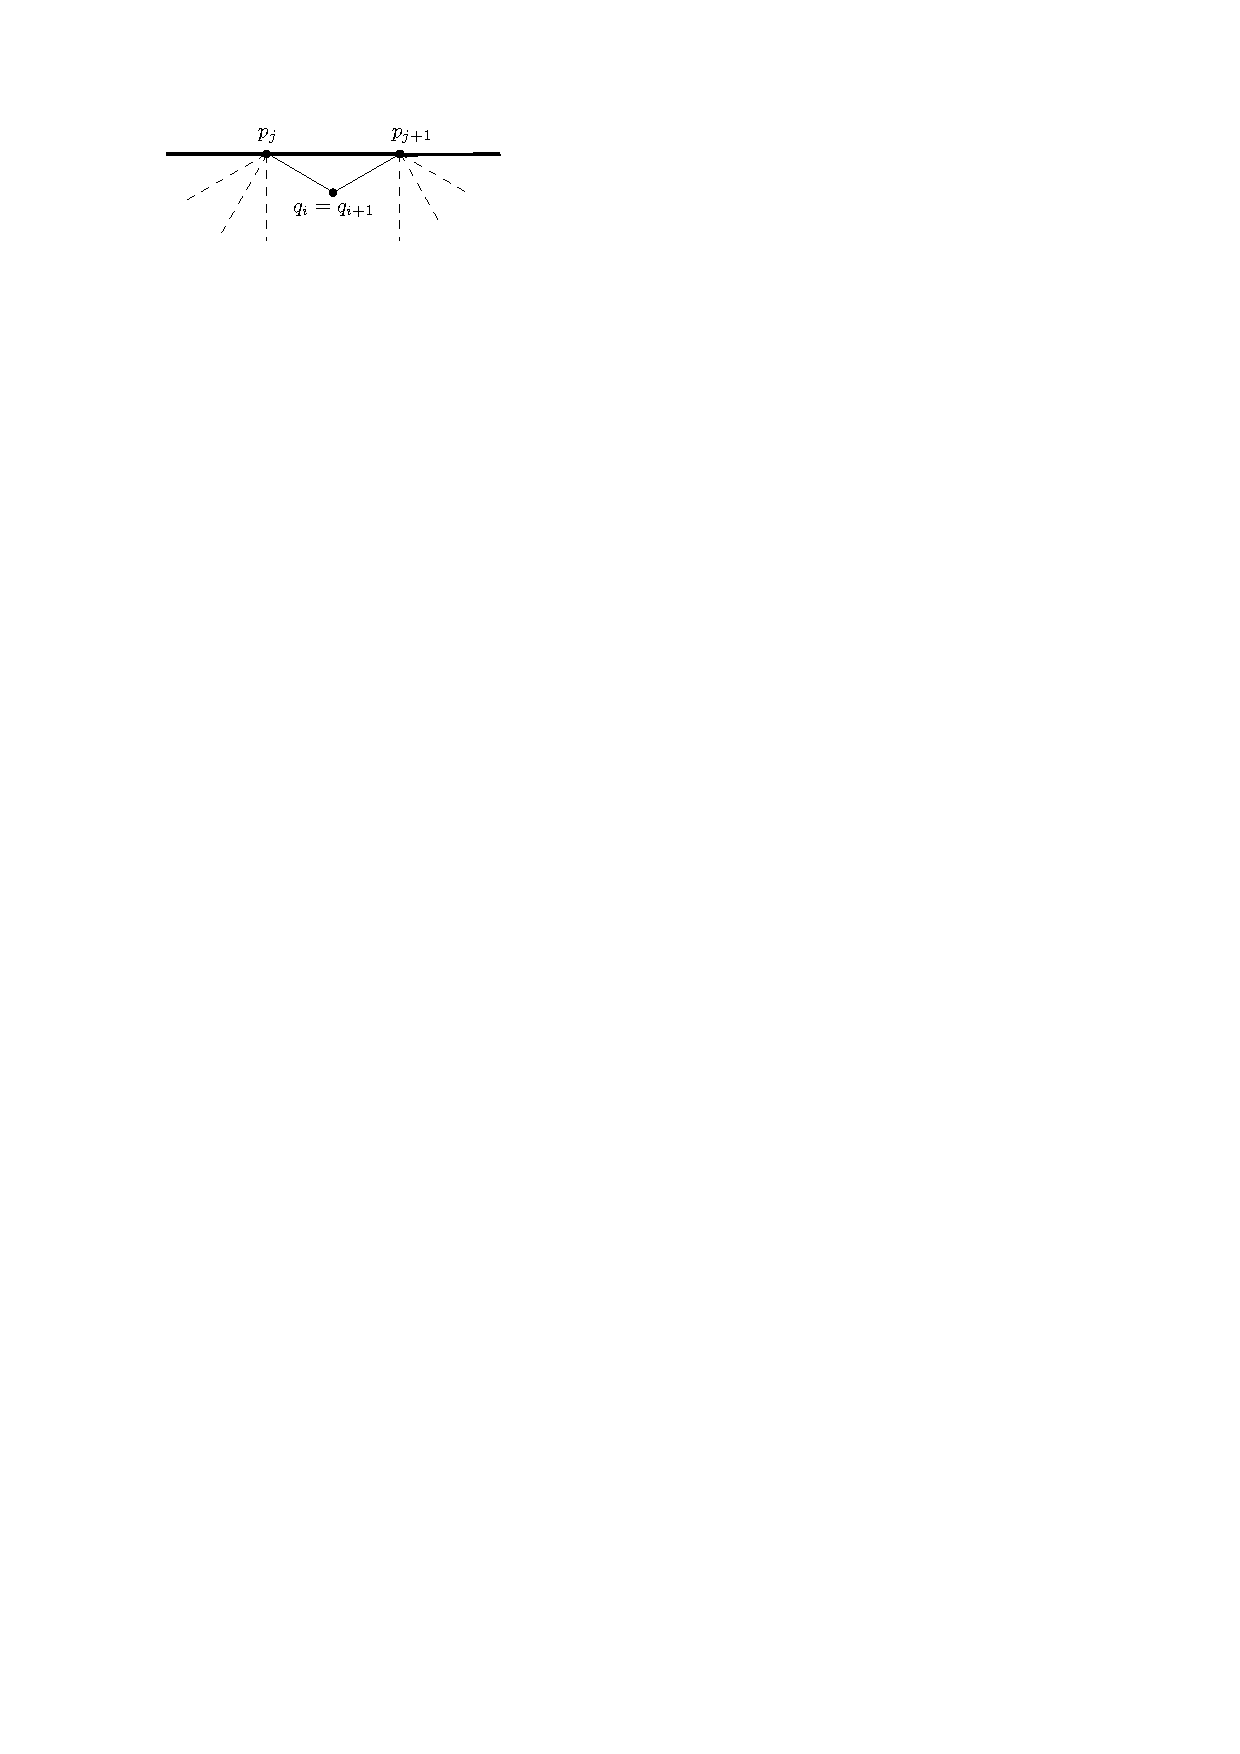
\includegraphics[width=\linewidth]{unifiedAlgo/img/walkProofB}
          \vspace{1cm}
          \caption{}
      \end{subfigure}
      \caption{The two main cases of the proof showing that $W$ is a walk}
      \label{fig:uni:walkproof}
    \end{figure}
  \end{proof}

  \begin{lemma}
    \label{lm:uni:neighborPath}
    The right neighbor path $Q$ is a path
  \end{lemma}
  \begin{proof}
    We already know $Q$ is a path by \ref{lm:uni:neighborWalk}. Hence we only have to show that $Q$ contains no duplicate vertices.

    Suppose that $Q$ has a duplicate vertex $q_i=q_j$ with $i<j$. Then this vertex must have been a neighbor to two different vertices in $P$. We denote these vertices $p_\ell$, $p_k$ with $\ell<k$. We are now in the situation of Figure \ref{fig:right:path}.

    By the order in which we added vertices to $Q'$, which is preserved by the removal of when we go to $Q$, we know that any vertices in-between $q_i$ and $q_j$ in $Q$ must be one of the following:
    \begin{enumerate}
      \item Adjacent to $p_\ell$ and in the interval $(q_i, p_{\ell+1})$ in $p_\ell$'s rotation.
      \item Adjacent to one of $p_{\ell+1},  p_{\ell+2},\ldots, p_{k-1}$ and to the right of $P$.
      \item Adjacent to $p_k$ and in the interval $(p_{k-1}, q_j)$ in $p_k$'s rotation.
    \end{enumerate}


    All three cases describe a vertex that lies in the interior of the cycle $q_i p_i p_{i+1} \ldots p_j$. However, since $P$ has no separating $2$-chords on the right this cycle must be empty. Therefore there are no vertices in-between $q_i$ and $q_j$. But $Q$ is a walk and $G$ is simple  so $Q$ has no subsequent duplicates. Hence $Q$ contains no duplicates at all and is thus a path.
  \end{proof}

  \begin{figure}[h]
    \centering
    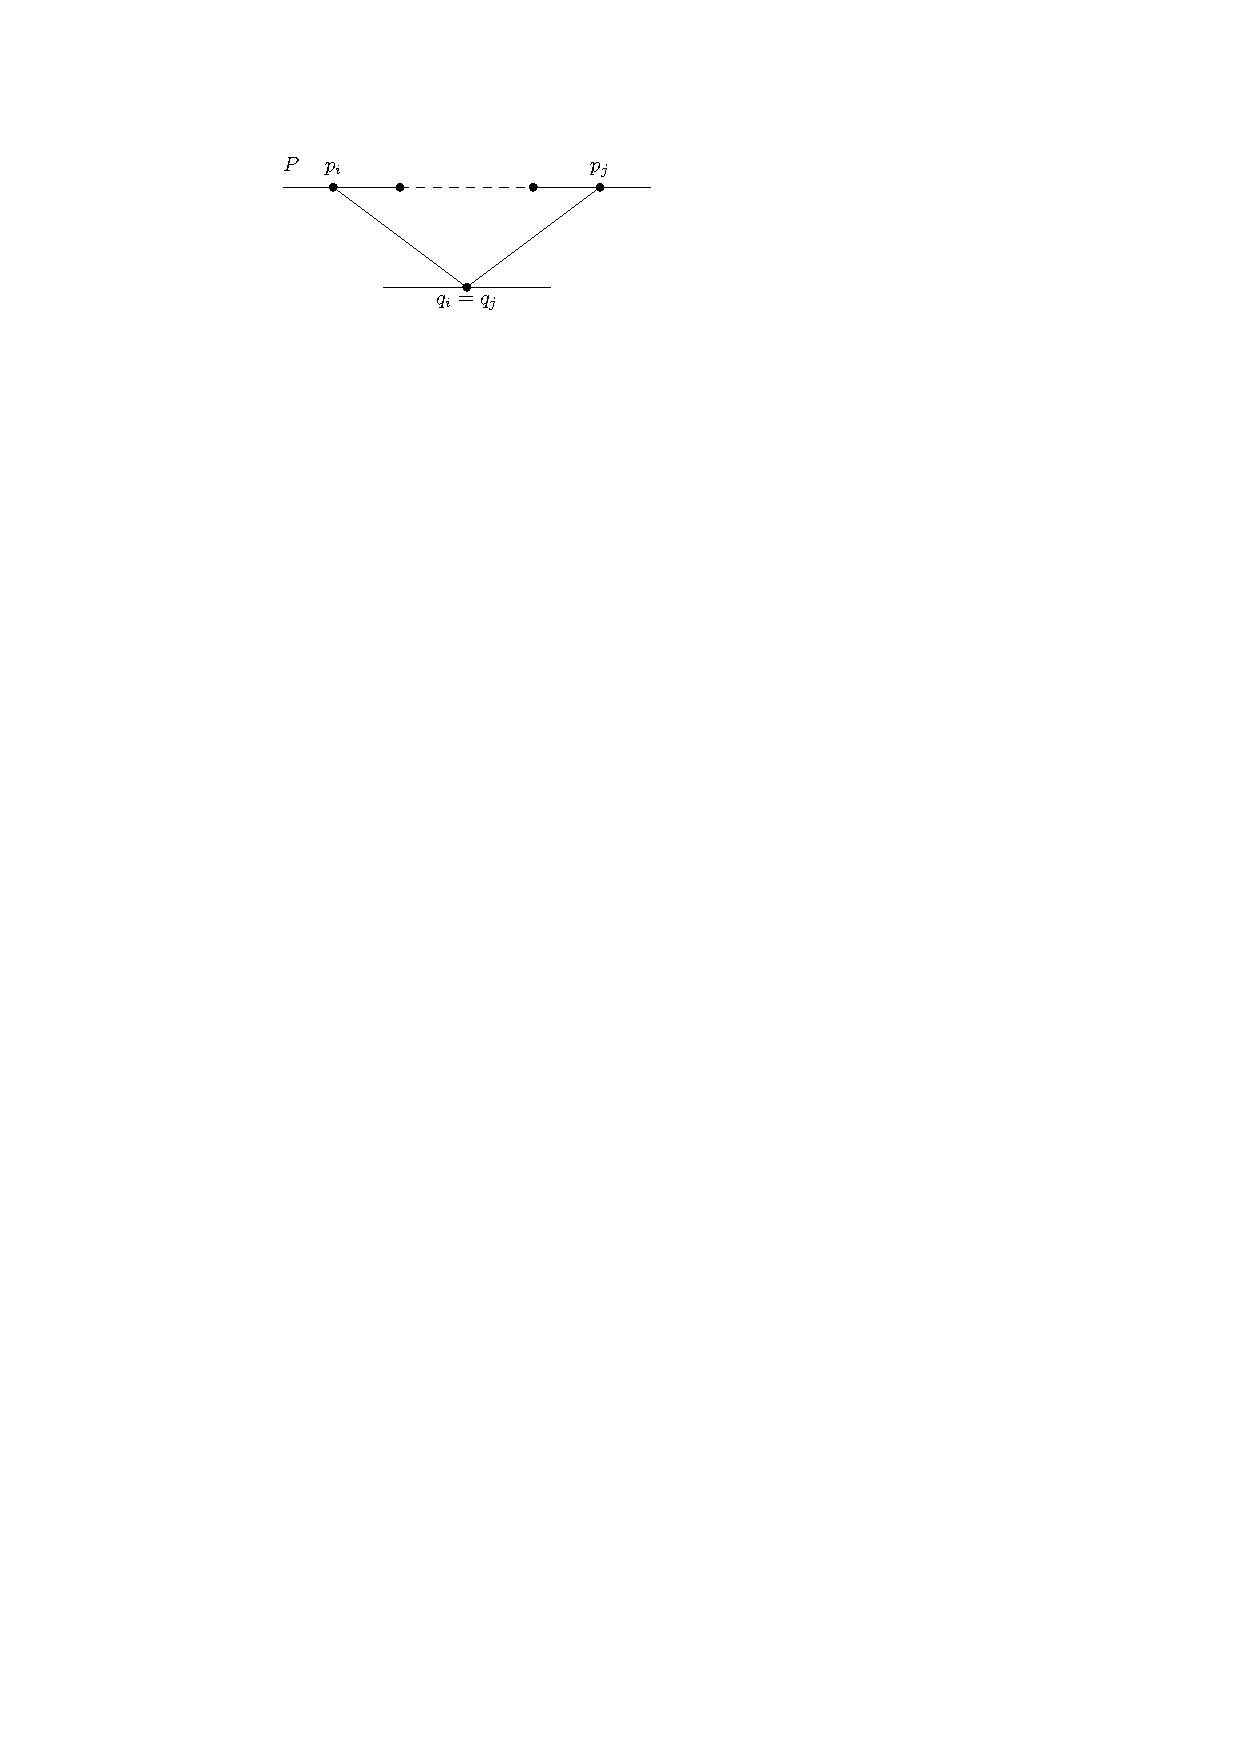
\includegraphics[scale=1]{unifiedAlgo/img/rightNeighbourwalk/neighborPathisPath.pdf}
    \caption{}
    \label{fig:right:path}
  \end{figure}

  \begin{lemma}
    \label{lm:uni:neighbourwalkNoInteriorVertex}
    The cycle $P \oplus \rev{Q}$ has no interior vertices.
  \end{lemma}
  \begin{proof}
    In the construction of the right neighbor path both cases in Figure \ref{fig:uni:walkproof} add a triangle to the interior with all vertices of the triangle in $W \oplus \rev{P}$. Hence the interior of $P \oplus \rev{Q}$ can be subdivided in a number triangles.

    Suppose there is a interior vertex in the cycle $P \oplus \rev{Q}$. Then the triangle containing this vertex is a separating triangle. Hence $P \oplus \rev{Q}$ has no interior vertices.
  \end{proof}


  \begin{lemma}
    \label{lm:uni:neighbourwalkChordFree}
    The left of a right neighbor path is chordfree.
  \end{lemma}
  \begin{proof}
    Suppose that the right neighbor path $Q = q_1 \ldots q_k$  has a chord on the left, say an edge between $q_i$ and $q_j$ with $i< j -1 $. There is a vertex $p_\ell \in P$ on the path such that $q_{i+1}$ is a neighbor of $p_\ell$ to the left of $p_\ell$. Consider now the cycle $P q_k \ldots q_{j+1} q_j q_i q_{i-1} \ldots q_1$
    (thick in Figure \ref{fig:uni:neihbourwalkChordFree}) this cycle has $q_{i+1}$ in its exterior. But then $p_\ell w_{i+1}$ is a crossing edge, which is forbidden.
    \fxwarning{TODO argue that an edge in the exterior is also imposible usning the path $P$. Maybe the vertex $q_{i+1}$ is actually in some cycle}

    \begin{figure}[h]
      \centering
      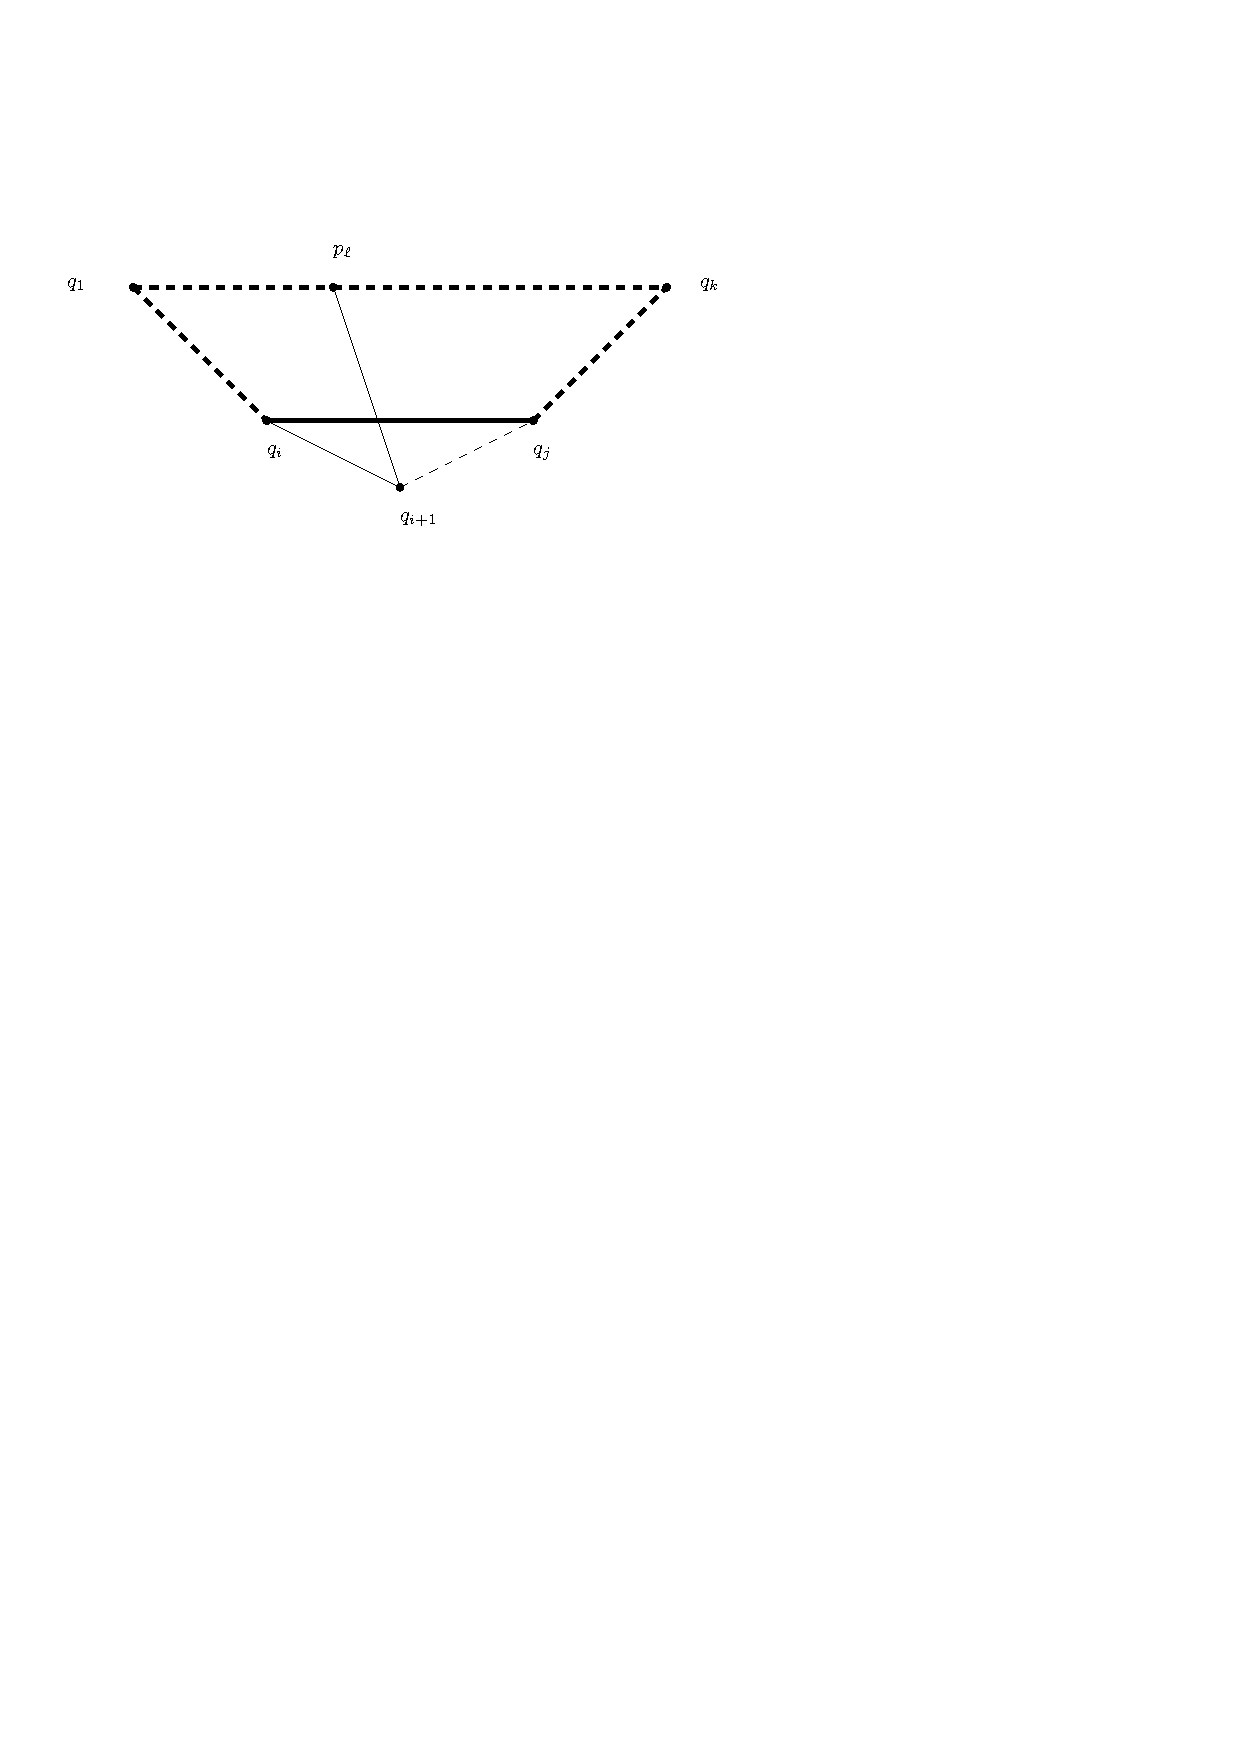
\includegraphics[scale=1]{unifiedAlgo/img/neighbourWalkChords}
      \caption{The construction in the proof of Lemma \ref{lm:uni:neighbourwalkChordFree}}
      \label{fig:uni:neihbourwalkChordFree}
    \end{figure}
  \end{proof}


\include{unifiedAlgo/sweepCycle}

%!TEX root = ../thesis.tex

\subsection{Flipping Blue $Z$'s}
\thispagestyle{plain}
\label{ss:flipBlueZ}

  The regular edge labeling provided by the sweepcycle algorithm of Section \ref{ss:sweep} is often vertically one-sided but we have not succeeded in proving that this is always the case.
  We prefer to obtain a vertically one-sided regular edge labeling since if we then recolor edges to subdivide large blue faces we cannot accidentally create many-sided vertical segments.
  In this section we modify the current regular edge labeling to make it vertically one-sided while maintaining the nice property of Lemma \ref{lm:sweep:NoTwoSplitsAboveEachOther}.


  A \emph{blue $Z$} is a path of three blue edges all in the same red face. A $Z$ has a \emph{midlle} edge, this is the second edge in this path.
  In the case that this regular edge labeling is not one-sided there must be a blue $Z$ as is proved in Lemma \ref{lm:zflip:blueZNorVertOneSided}.
  \begin{lemma}
    \label{lm:zflip:blueZNorVertOneSided}
    A regular edge labeling is not one sided if and only if it contains a blue $Z$
  \end{lemma}
  \begin{proof}
    Consider a regular edge labeling that is not one-sided, then it contains a red face of which both boundary paths are of length at least $3$. However since the interior faces of $G$ are triangles there must then be a blue $Z$ in this face.
    On the other hand, if a face contains a blue $Z$ it can not be one-sided.
  \end{proof}

  \begin{figure}[h]
    \centering
    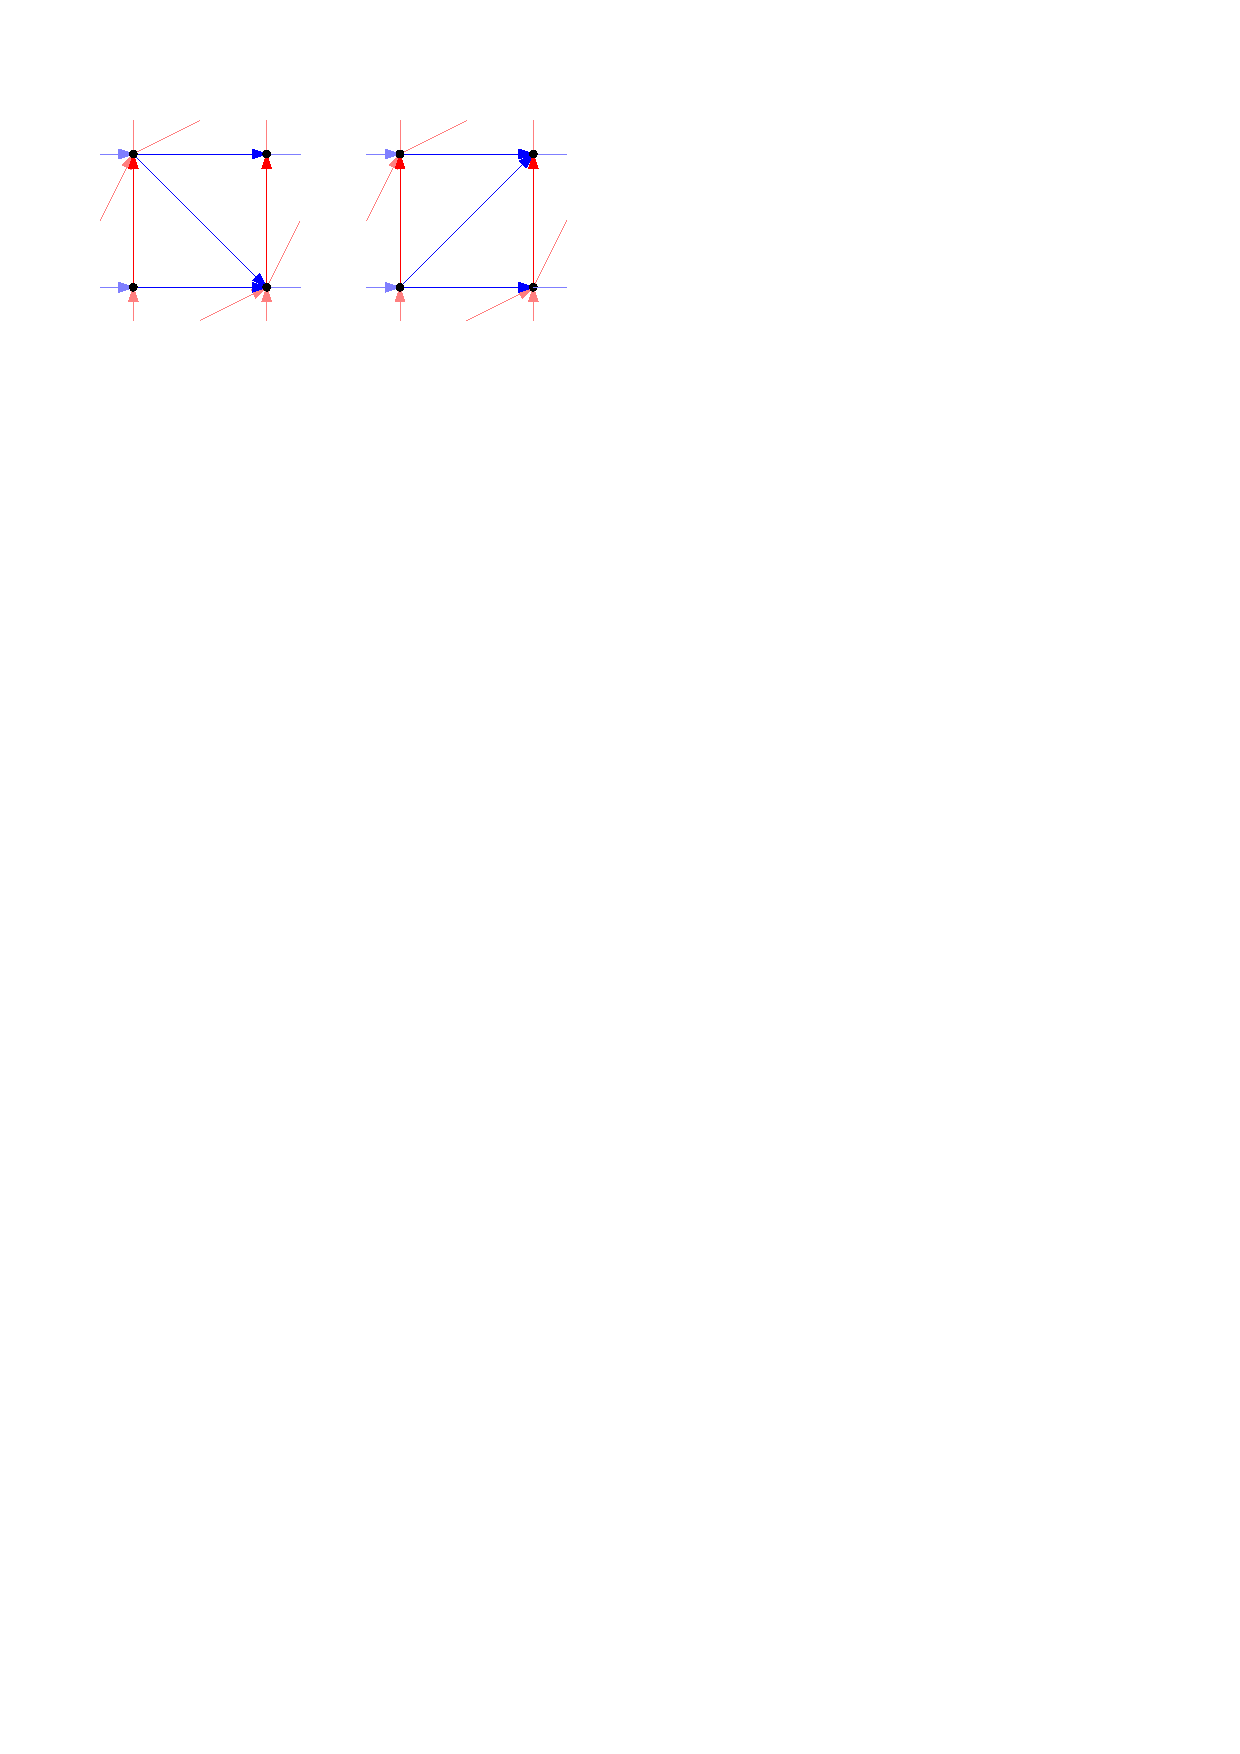
\includegraphics[scale=1]{unifiedAlgo/img/zflip/blueZ.pdf}
    \caption{The two possible blue $Z$'s}
    \label{fig:zflip:blueZ}
  \end{figure}

  As long as the regular edge labeling is not vertically one-sided we find such a blue $Z$ and recolor its middle edge as in Figure \ref{fig:zflip:flip}. We call this a \emph{flip} and we will say that this edge is \emph{flipped}.
  Note that both flips transfer a valid regular edge labeling to another valid regular edge labeling. If the interior vertex condition was fulfilled in Figure \ref{fig:zflip:blueZ} then it is also fulfilled in Figure \ref{fig:zflip:flip}.

   We repeat these flips until the regular edge labeling is vertically one-sided.
   Since every flip reduces the number of blue edges by one this is a finite procedure.

  \begin{figure}[h]
    \centering
    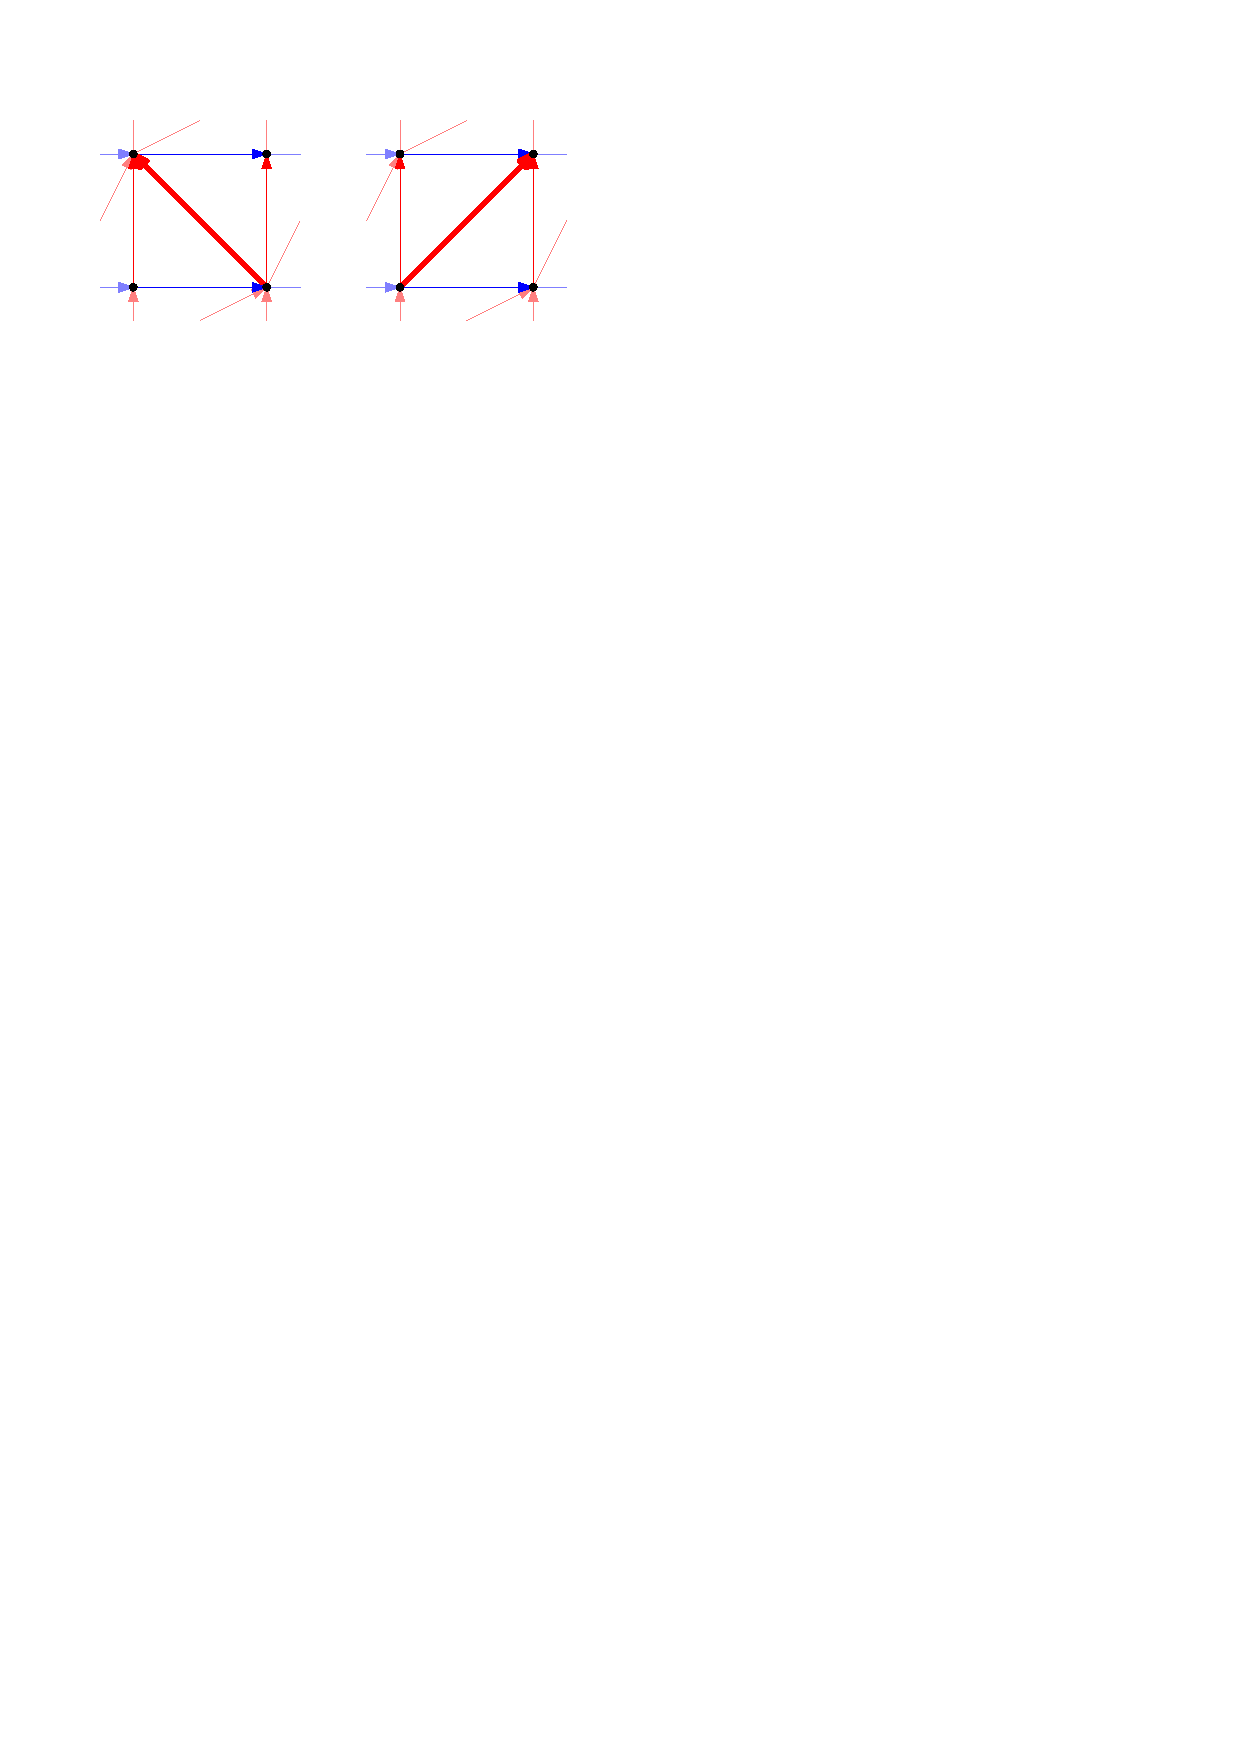
\includegraphics[scale=1]{unifiedAlgo/img/zflip/flip.pdf}
    \caption{The flip}
    \label{fig:zflip:flip}
  \end{figure}

  \begin{lemma}
    \label{lm:sweep:vertOnsided}
    The result is a rectangular edge labeling and vertically one-sided
  \end{lemma}
  \begin{proof}
    By construction we flip all blue $Z$'s. If we do not have any more $Z$'s then the remaining regular edge labeling is vertically one-sided by Lemma \ref{lm:zflip:blueZNorVertOneSided}.
  \end{proof}

  \begin{lemma}
    \label{lm:sweep:NoTwoSplitsAboveEachOtherVertOnesided}
    Let $v$ be any splitvertex. Then the subsequent vertex on the bottom path $w$ can not be the handle of a large topfan.
  \end{lemma}

  \begin{proof}
    Note that this is the same statement as is provided in Lemma \ref{lm:sweep:NoTwoSplitsAboveEachOther}. We will show that the operation of flipping $Z$'s does not compromise the validity of this lemma.

    Not that the flips can only reduce the number of split vertices. Hence it suffices to show that the statement still holds for all previously existing split vertices.


    For a split vertex $v$ adjacent to $\pS$ we can note that the edge $vw$ will not be flipped because it can not be a middle edge. Hence $w$ is still on the bottom path and still not the handle of a big topfan.

    If $v$ is a split vertex due to a chord let us note the following.
    The edges of $\P$ and $ab$ in Figure \ref{fig:sweep:botomPathChord} can not have been flipped since then we would find a monochromatic red triangle while a flip leads to another valid regular edge labeling. Hence $w$ is still on the bottom path trough $v$ and still can not be the handle of a large topfan.
  \end{proof}


%!TEX root = ../thesis.tex

\subsection{Top Fan flips}
\thispagestyle{plain}
\label{ss:fanflip}

The second stage of the algorithm will consist of flipping most large topfans. The first stage of the algorithm finished by computing a vertically one-sided \rel (Lemma's \ref{lm:sweep:REL} and \ref{lm:sweep:vertOnsided}) that never has a split next to a topfan handle along the rightmost edge of the split (Lemma \ref{lm:sweep:NoTwoSplitsAboveEachOtherVertOnesided}).

Using some local recoloring (\emph{flips}) on the topfans we will maintain a onesided REL (Lemma \ref{lm:topfan:oneSidedREL}) and make sure that large topfans only occur in very specific situations (Lemma \ref{lm:topfan:remainingTopfans}).

Our flips differ depending on whether we we encounter a split and or merge in the bottom boundary path. Refer to Figure \ref{fig:fanflip:fanflips} for the different kinds of topfanflips.


\begin{figure}
    \centering
    \begin{subfigure}[b]{0.8 \textwidth}
        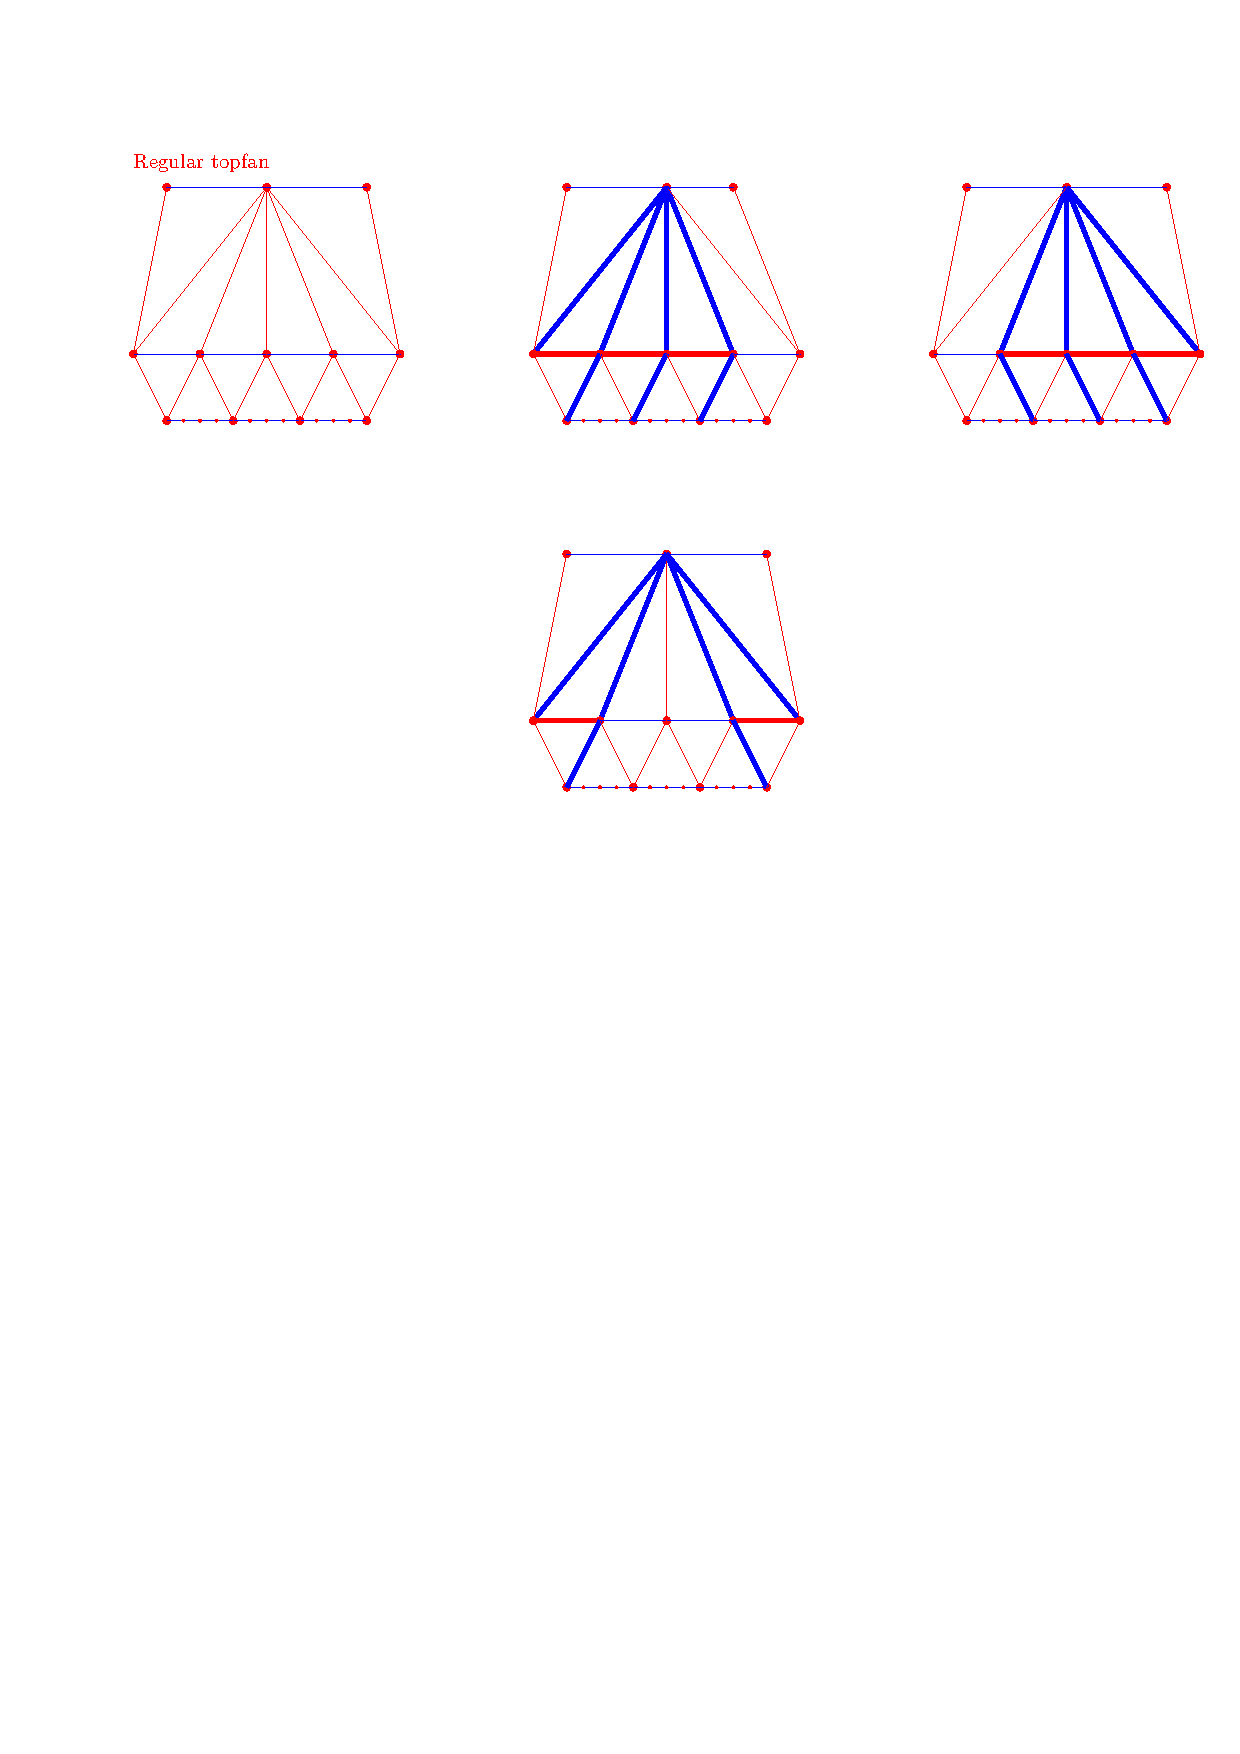
\includegraphics[width = \textwidth]{topFanFlips/img/regular}
        \caption{The regular topfanflip}
        \label{fig:fanflip:regular}
    \end{subfigure}
    ~
    \centering
    \begin{subfigure}[b]{0.45 \textwidth}
        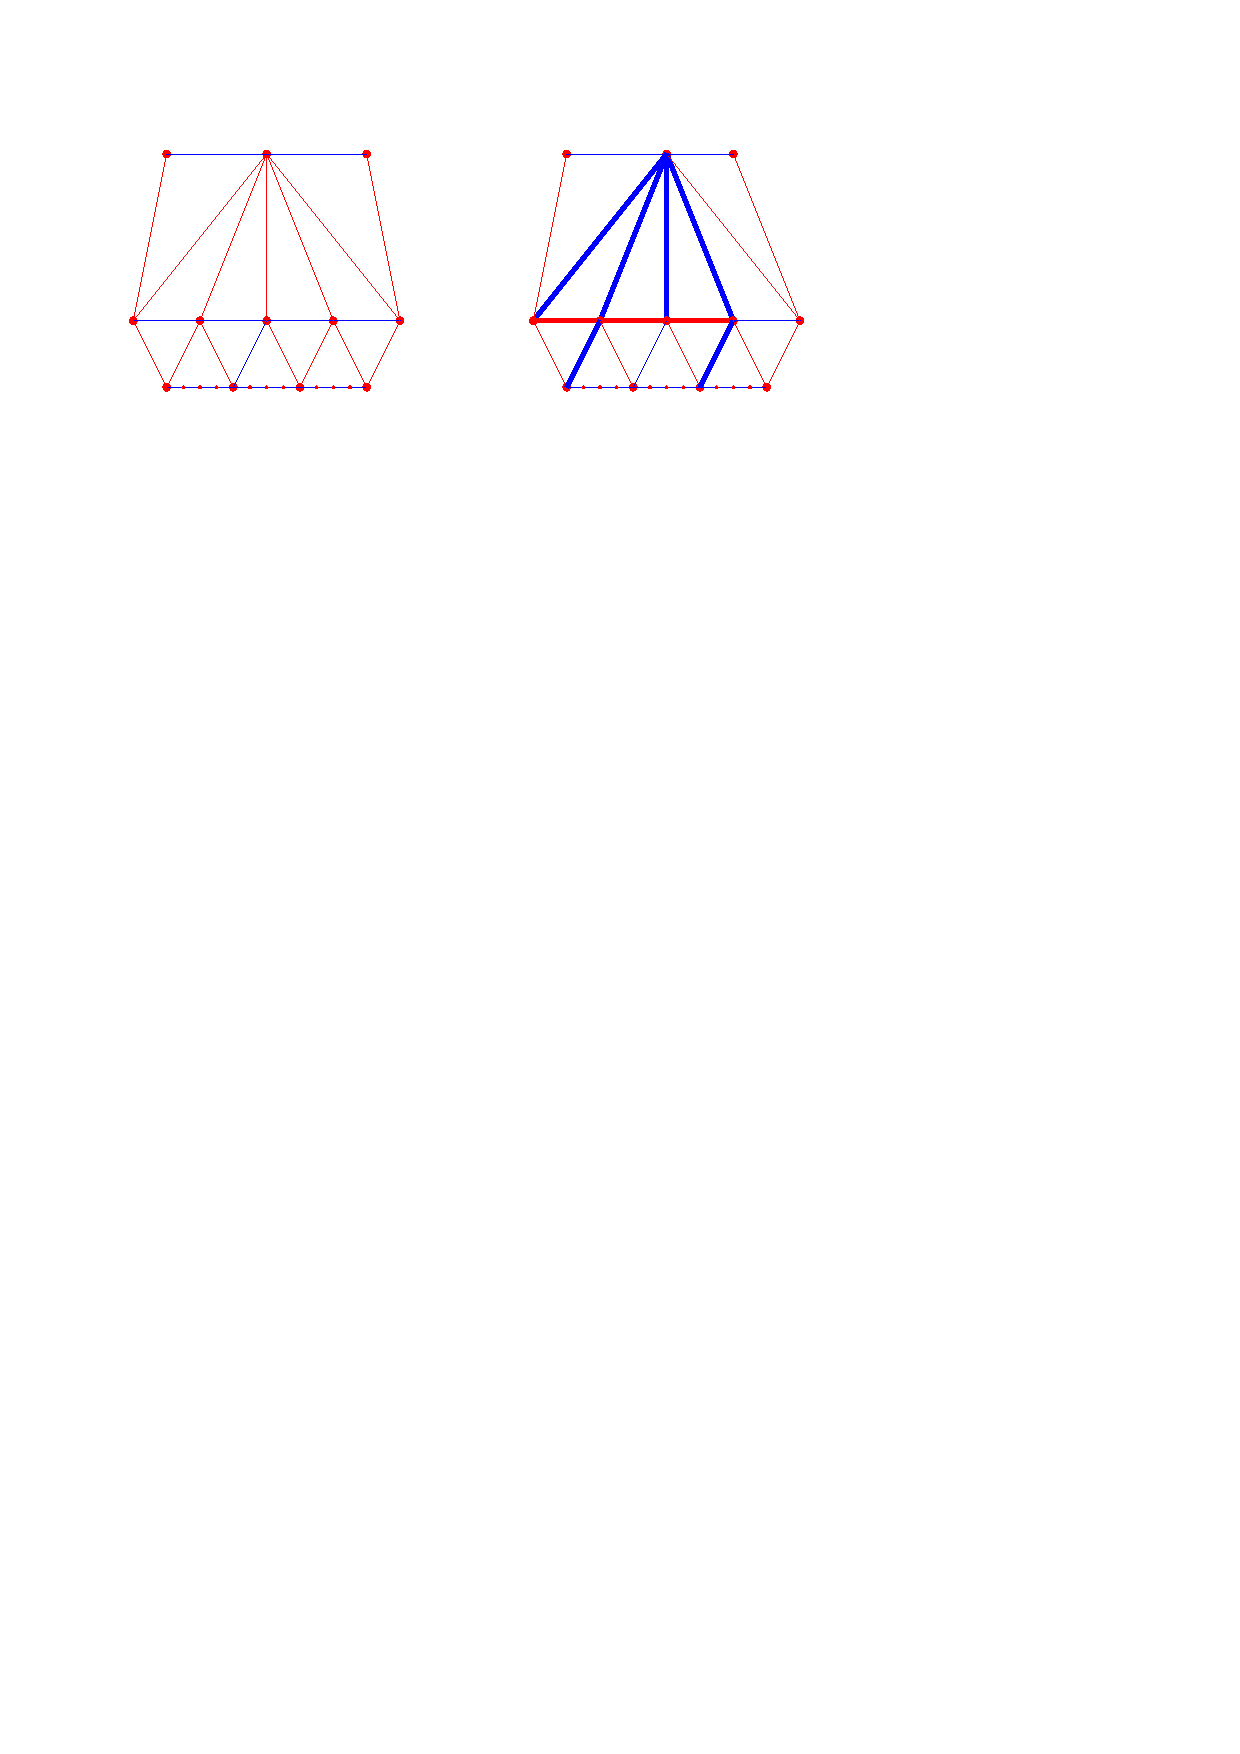
\includegraphics[width = \textwidth]{topFanFlips/img/merge}
        \caption{Topfanflip above a merge}
        \label{fig:fanflip:merge}

    \end{subfigure}
    ~
    \begin{subfigure}[b]{0.45 \textwidth}
        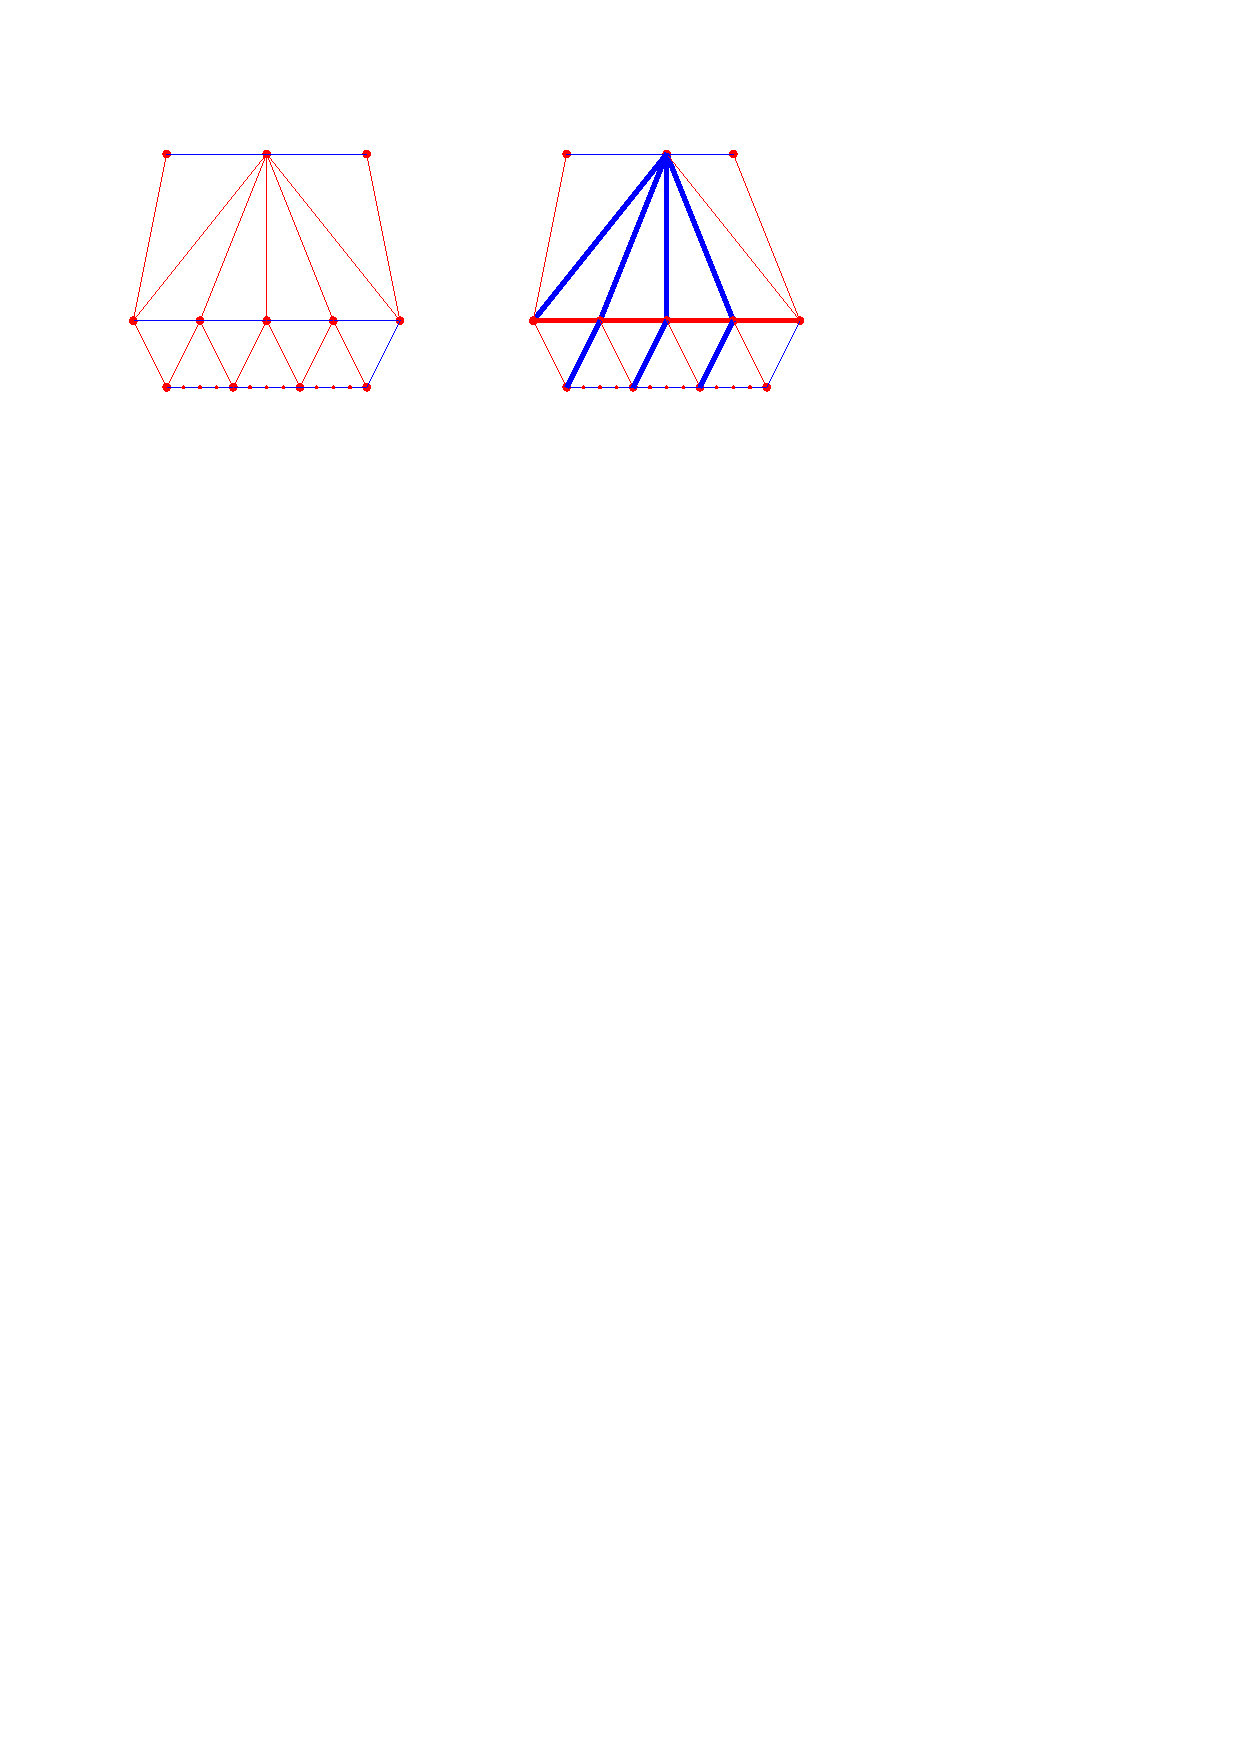
\includegraphics[width =\textwidth]{topFanFlips/img/mergeend}
        \caption{Topfanflip next to merge. Note the additional red edge.}
        \label{fig:fanflip:mergeLastVertex}

    \end{subfigure}
    \centering
    \begin{subfigure}[b]{0.45 \textwidth}
        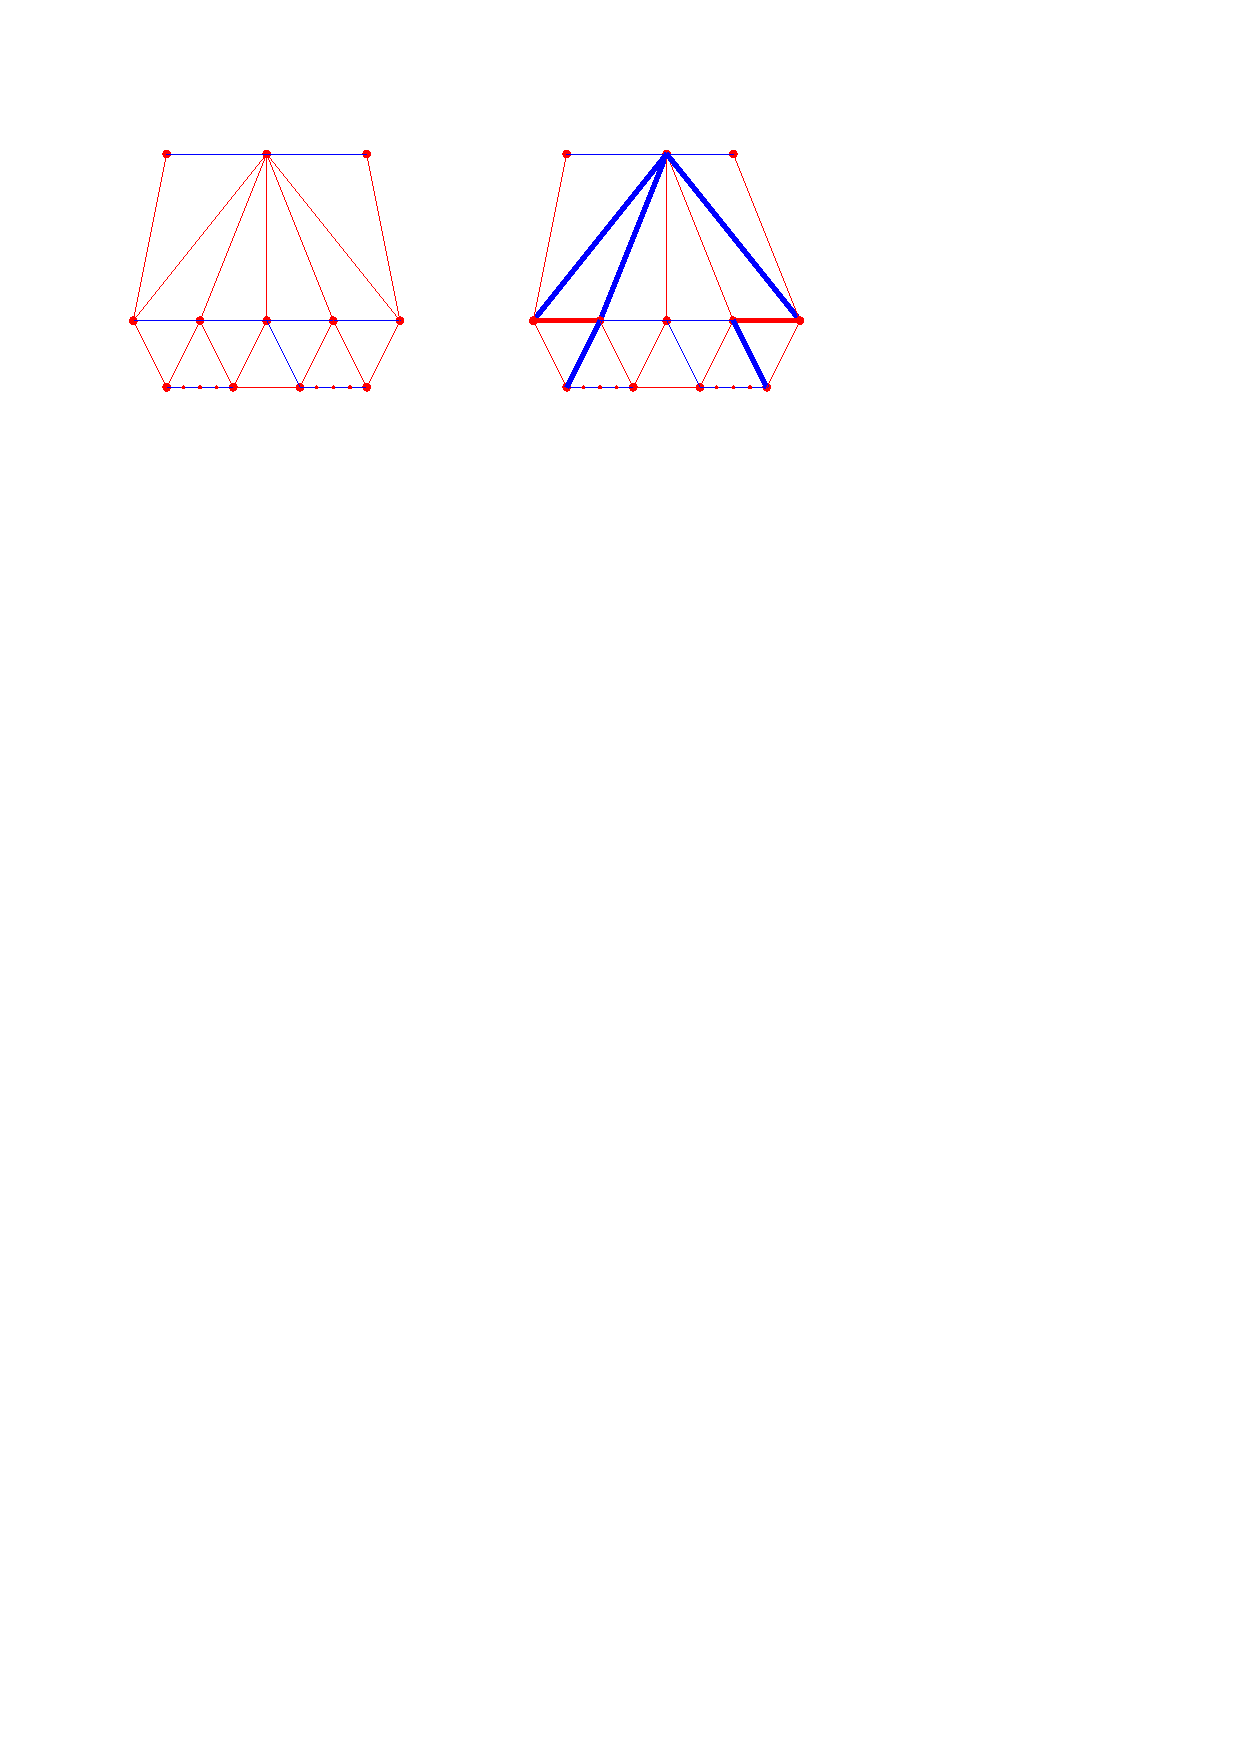
\includegraphics[width = \textwidth]{topFanFlips/img/split}
        \caption{Above a split we stop}
        \label{fig:fanflip:split}

    \end{subfigure}
    ~
    \begin{subfigure}[b]{0.45 \textwidth}
        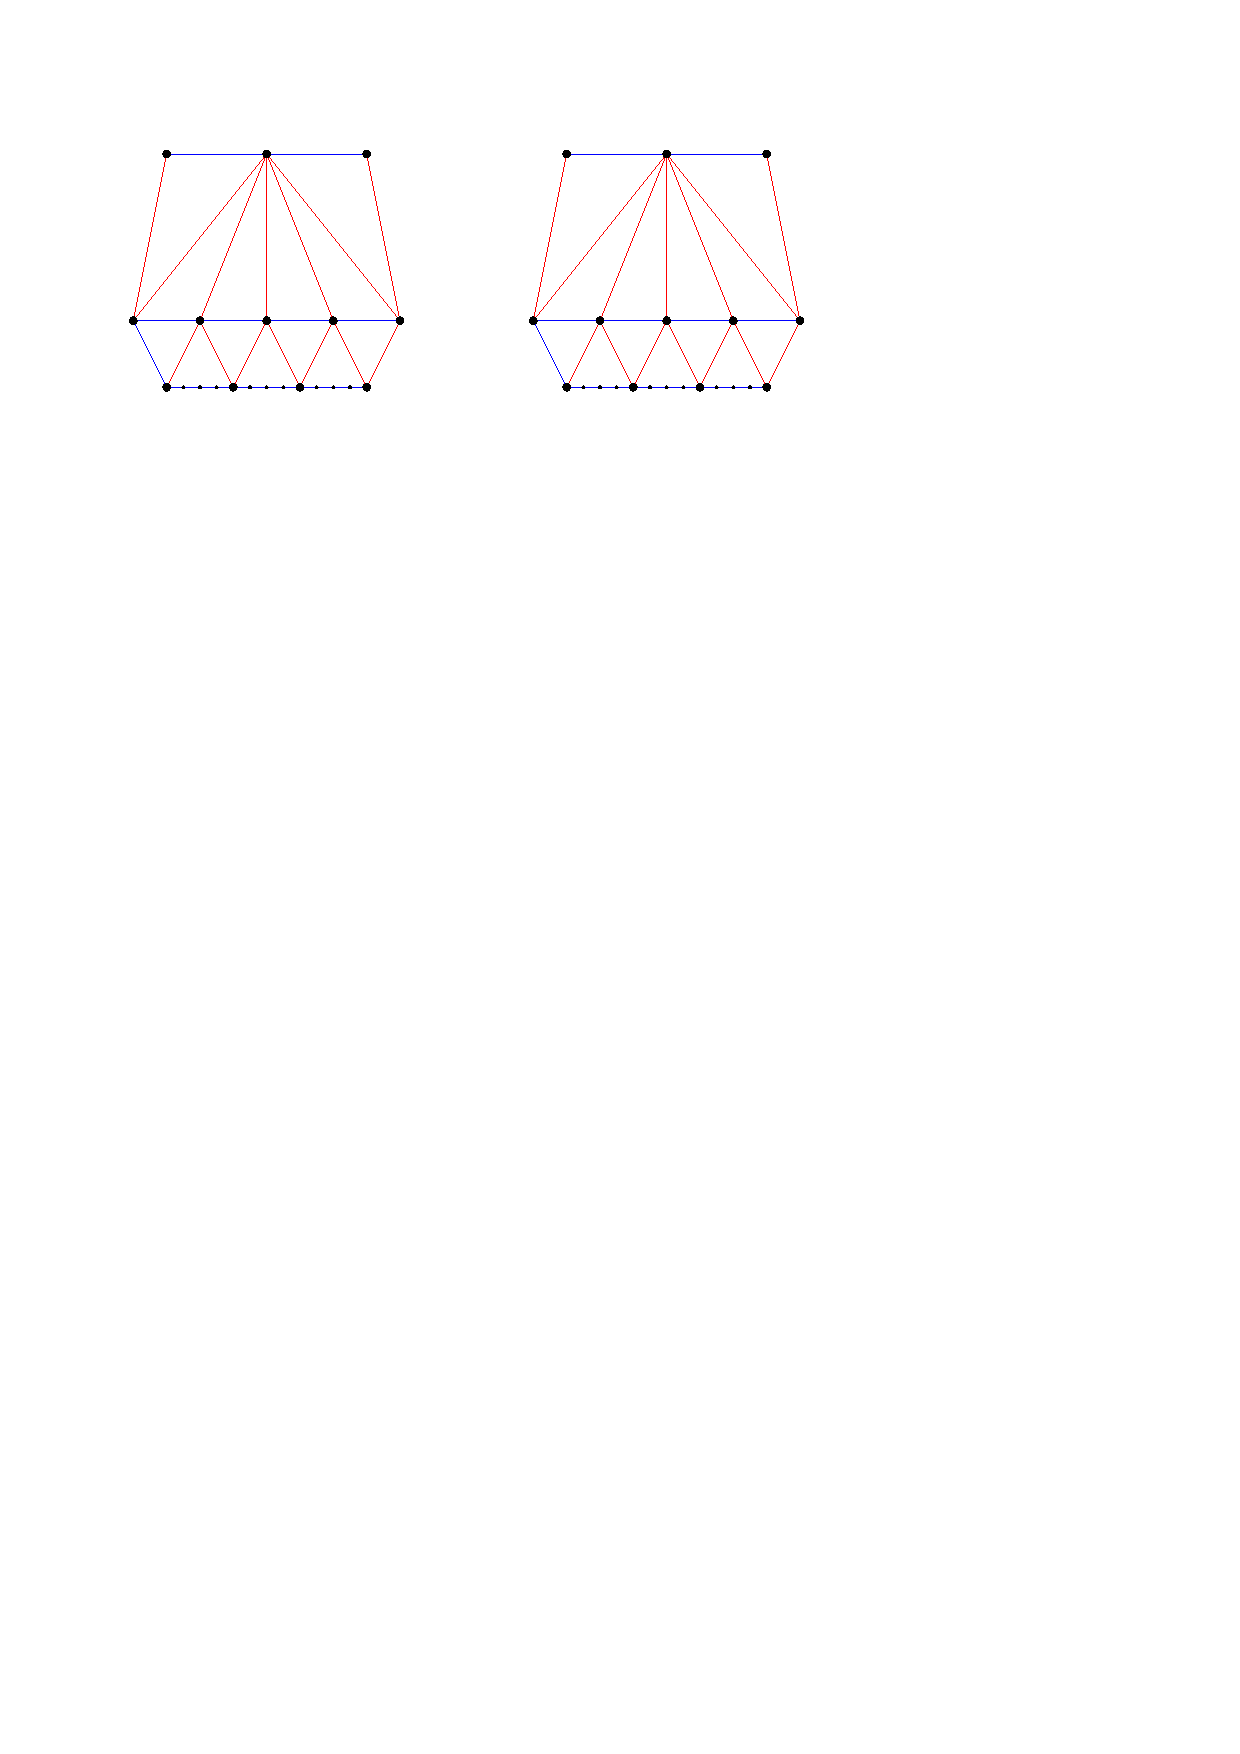
\includegraphics[width =\textwidth]{topFanFlips/img/splitfront}
        \caption{If the split is on the first vertex we do not flip at all}
        \label{fig:fanflip:splitFirstVertex}

    \end{subfigure}

    \caption{}
    \label{fig:fanflip:fanflips}
\end{figure}


%\fxnote{We could make structure of the fence below the topfan more explicit. But we do not really need this}

We consider all faces we have in order from first created to last created.

\mypar{Flipping topfans}
A topfan is above a number of edges of the bottom fence of the face containing the topfan. These edges are the rim of the fan.

We flip the topfan along the rim starting at the first vertex and ending at the the vertex \textbf{before} the first split or $\pS$ adjacent vertex or the vertex \textbf{before} the last vertex. This can imply that we do not flip any edges (in the case that the first vertex is a split vertex or $\pS$-adjecent).


For the first vertex $v_1$ we recolor the adjacent outer edge of the topfan. For subsequent vertices $v_i$ we recolor the rim edge between this vertex and the previous vertex $v_{i-1}$ red and we recolor the edges adjacent to this edge in the rotation at $v_i$ blue (if they weren't already blue).

If we stop flipping before a merge vertex $v_{i+1}$ we flip and additional edge $v_i v_{i+1}$ along the rim.

Examples of this procedure are given in the following paragraph.


\mypar{Examples}
If the rim has no merges or splits we execute the topfanflip depicted in Figure \ref{fig:fanflip:regular}. We color all but the rightmost fan edge blue, color all but the rightmost rim edge red. And color the left sides of all topfans below this topfan in the face below the current face blue.

If the rim consists of only merges we easily adept a topfanflip to this situation. We simply do not flip the edge merging in as depicted in Figure \ref{fig:fanflip:merge}.

A special case is given by a merge on the last vertex on the bottom edges of the top fan. In that case we flip all rim edges (even the last one) to prevent a blue $Z$ from forming. See figure \ref{fig:fanflip:mergeLastVertex}.

Splits are more difficult to handle. We are unfortunately unable to keep flipping once we hit a split hence we stop before we get that far. See Figure \ref{fig:fanflip:split}. It this happens on the first vertex we do not flip at all, see Figure \ref{fig:fanflip:splitFirstVertex}.

\mypar{The result}
Before the topfanflips we had a vertically one-sided REL. Afterwards we still have a vertically one-sided \rel as we will prove in Lemma \ref{lm:topfan:oneSidedREL}. Moreover we have no large top-fans except for some controlled cases as we will prove in Lemma \ref{lm:topfan:remainingTopfans}.

\begin{lemma}
  \label{lm:topfan:oneSidedREL}
  If the graph was onesided before a topfanflip it is still onesided after such a flip in the regular and merge cases.
\end{lemma}
\begin{proof}
  We invite the reader to take another look at Figure \ref{fig:fanflip:fanflips}.
  Let us first consider the regular case. Since the edge  $v_n w_m$ is red (otherwise we would have a merge) this change does not produce any blue $Z$'s.

  Let us also consider the other merge cases. Due to the clever recoloring these also do not lead to a merge.
  %However they can lead to a face starting with a large topfan. We will later see this is a controlled topfan.

  It is clear the split cases also do not produce a blue $Z$.

  Since any south-adjecnt fan is treated like a split fan we also do not create $Z$'s  in these cases.
  %But the topfans are again controlled. As we will see in the next section.
\end{proof}


\begin{lemma}
  \label{lm:topfan:remainingTopfans}
  In the remaining faces every large topfan is in one of the following two situations.
  \begin{enumerate}
    \item  This topfan is at the start of the face
    \item  This topfan is in the middle of the face and its left outer rim vertex is a split.
  \end{enumerate}
\end{lemma}
\begin{proof}
  All topfans are manipulated in such a way that they start a new face unless the left outer rim vertex is a split. In that case we do not flip at all.
\end{proof}


%!TEX root = ../thesis.tex

\section{Blue face subdivision}
\label{s:subdiv}


At this point we have a vertically one-sided graph (due to Lemma \ref{lm:topfan:oneSidedREL}) without large topfans except possibly for the locations provided in Lemma \ref{lm:topfan:remainingTopfans}.

\mypar{Outline}
In this stage we are going to recolor edges in all blue faces to make all of them $d+1$-sided. We will start at the bottommost face in the creation order (which we will have to recalculate after the topfanflips, but every REL has one). And we will recolor some if it's edges if a blue face that is to large will appear. \fxnote{I may need to expand a bit more on this order}

We then mark the edges on the top boundary path of this face above the recolored edges as \emph{loaded}. This means that we will try to not flip above these edges in future iterations of the algorithm.

Then we continue with the next face in the order we just calculated.


\mypar{Loads}
As is mentioned above we will mark some edges using so-called \emph{loads}, we will in the rest of the section refer to these edges as \emph{loaded}. The exact use of these loaded edges will become clear in the rest of this section. But as is mentioned above we try to not flip above these edges.

It is important to note that if we load any blue edge we regard any other blue edge sharing at least one vertex with this edge to be loaded as well. The occurrence of this phenomenon will be called \emph{putting trough a load}. An example can be seen in Figure \ref{fig:subdiv:putTrougLoad}.

\begin{figure}[h]
  \centering
  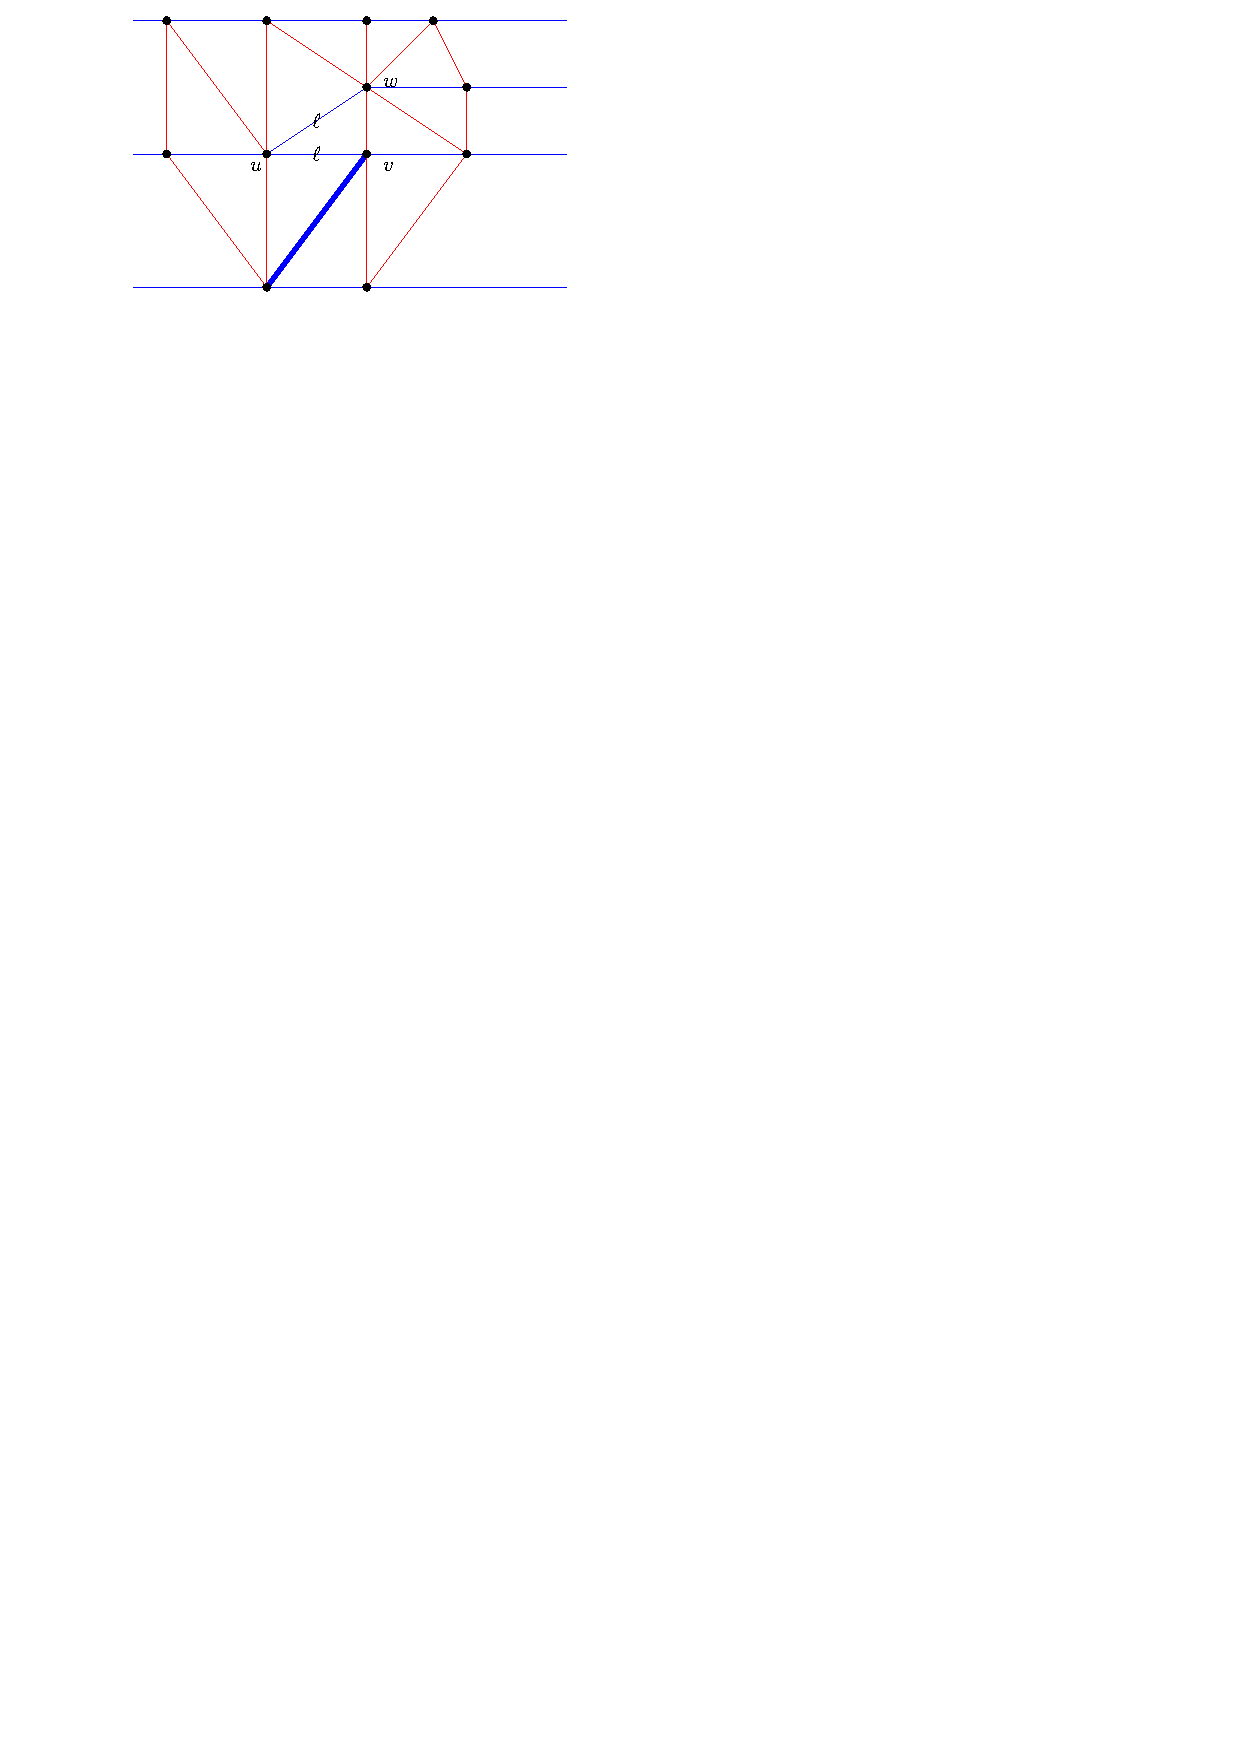
\includegraphics[scale=1]{blueFaceSubdivision/img/puttingTroughLoad.pdf}
  \caption{The fat edge is flipped. Hence we mark $uv$ as loaded. Via the mechanism of putting trough load $uw$ also becomes marked as loaded.}
  \label{fig:subdiv:putTrougLoad}
\end{figure}


\mypar{Step requirements}
We flip edges in each face, taking into account loads on the bottom fence. Such that

\begin{enumerate}
  \item We never load the edge next to a split/merge
  \item We never load two adjacent edges
\end{enumerate}

It's important to note that we put trough edge loads on splits and merges

Because we do this we can also say the following

\begin{lemma}
  \label{lm:}
  On the bottom boundary path of every face we never find two subsequent loaded edges. Even when we put trough loads on splits and merges.
\end{lemma}
\begin{proof}
  A single face would never load two subsequent edges. Hence the only way to get two subsequent loaded edges is using different faces and thus splits and merges.

  However due to never flipping next to a split/merge we never get subsequent loaded edges.
\end{proof}


\subsection{Faces without large topfans in the midlle}
Let us first consider the base case: no failed top fan flips and thus all topfans are of size exactly $2$.

\begin{lemma}
  \label{lm:subdiv:withoutTopfan}
  We can subdivide any blue face without large topfans into 5-sided chunks while obeying the load rules above.
\end{lemma}

\begin{proof}
  A worst case example is given in Figure \ref{fig:subdiv:worstCase}.

  \begin{figure}[h]
    \centering
    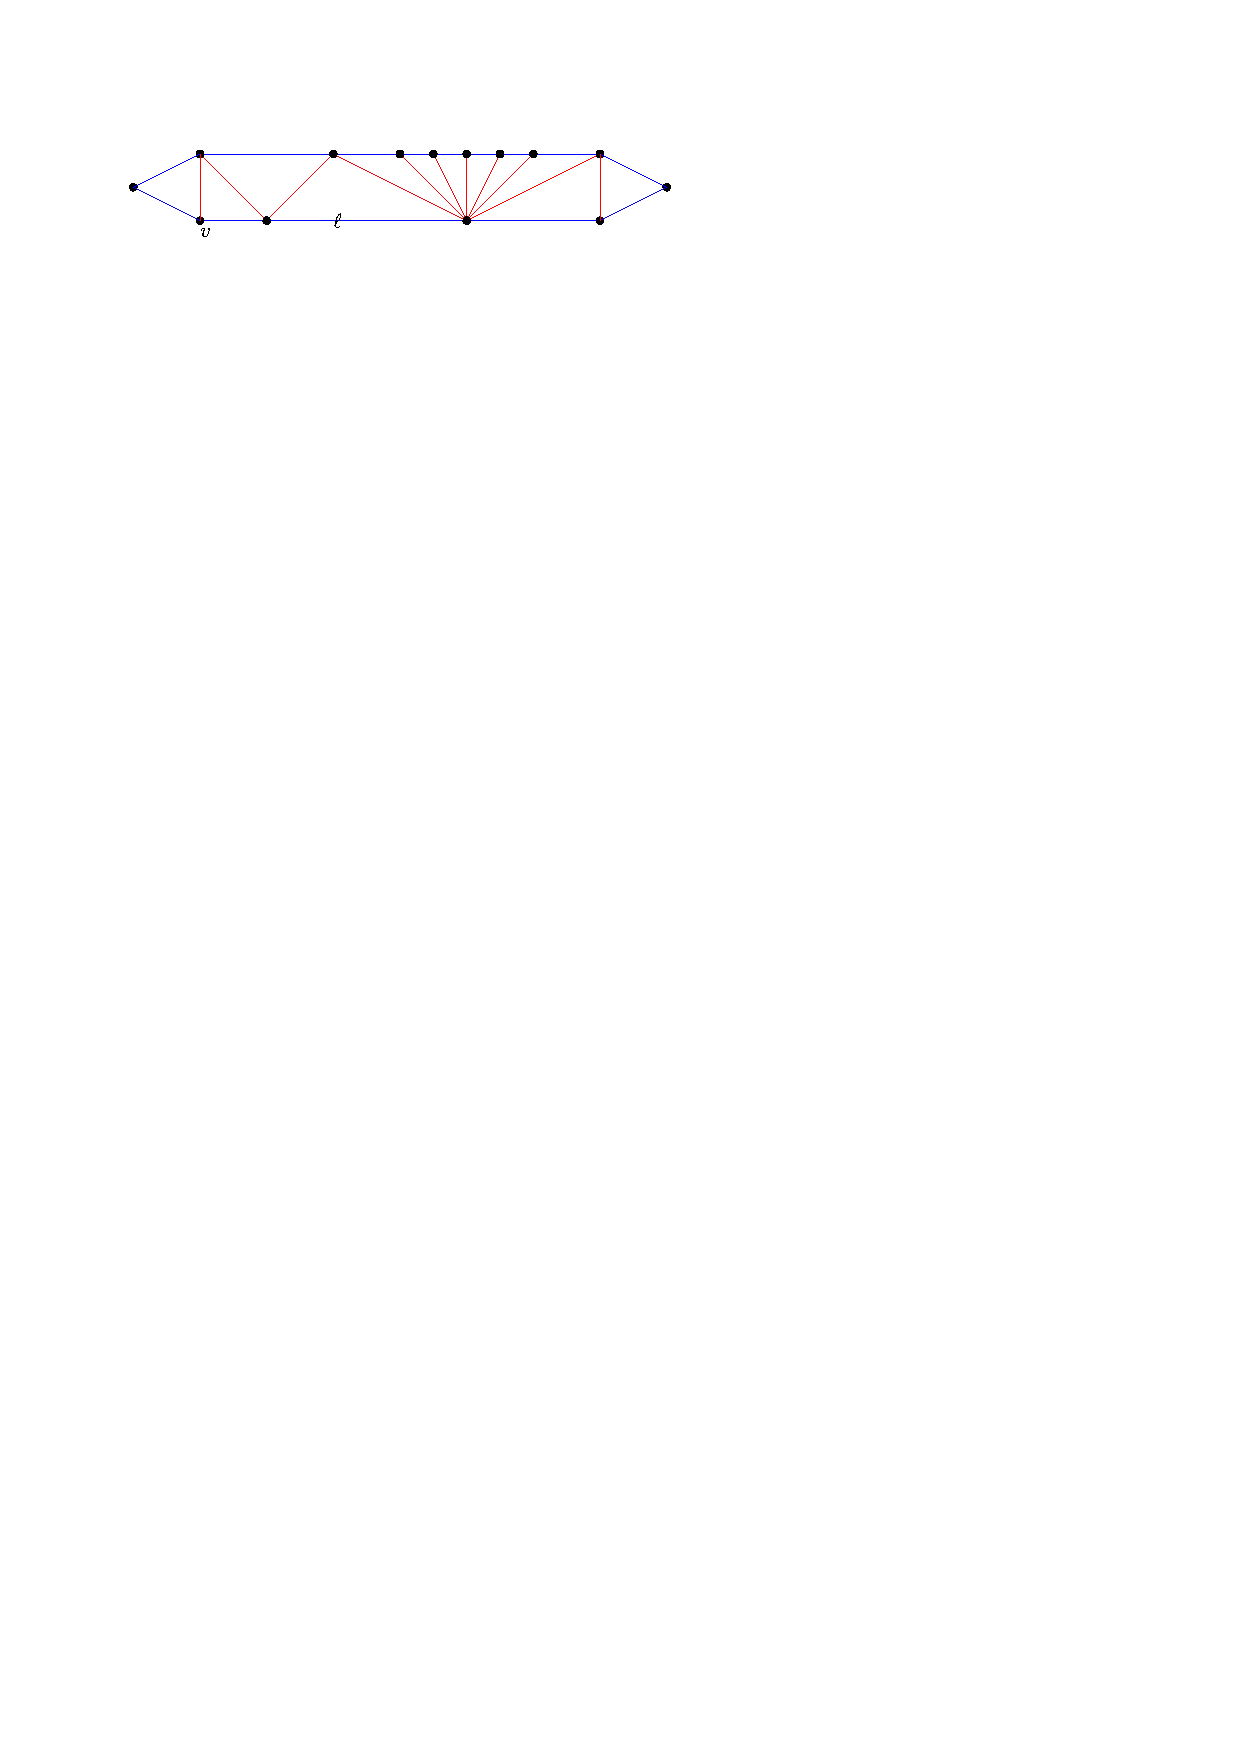
\includegraphics[scale=1]{blueFaceSubdivision/img/worstCase}
    \caption{A worst case blue face. We don't flip any edge in this face.}
    \label{fig:subdiv:worstCase}
  \end{figure}

  Note that we can flip to the right above each edge in the bottom boundary path.

  We will look at the vertex on the bottom fence that's adjacent to the freshly flipped edge, or if we haven't flipped an edge yet the vertex next to the split (and we will call it $v$). The following are then the rules for flipping above the edges following $v$.
  \begin{enumerate}
    \item We don't flip above the first edge.
    \item We flip above the second edge if it's unloaded.
    \item Otherwise we flip above the third edge.
    \item We never flip next to the merge the merge
  \end{enumerate}

  When flipping above a edge we always flip the right edge above that edge.

  The first edge give us the required separation of loaded edges along the top boundary path. The other items make sure we obey the other rules in a straightforward manner.

  The worst case is given by a combination of the last two items. We would in that case want to flip above the third edge. But we don't because the next edge is the merge. This gives at worst 5 edges along the whole bottom boundary path and hence a $4$-sided face.



\end{proof}

See Figure \ref{fig:subdiv:sampleExecution} for a sample execution of the algorithm described in Lemma \ref{lm:subdiv:withoutTopfan}.

\begin{figure}[h]
  \centering
  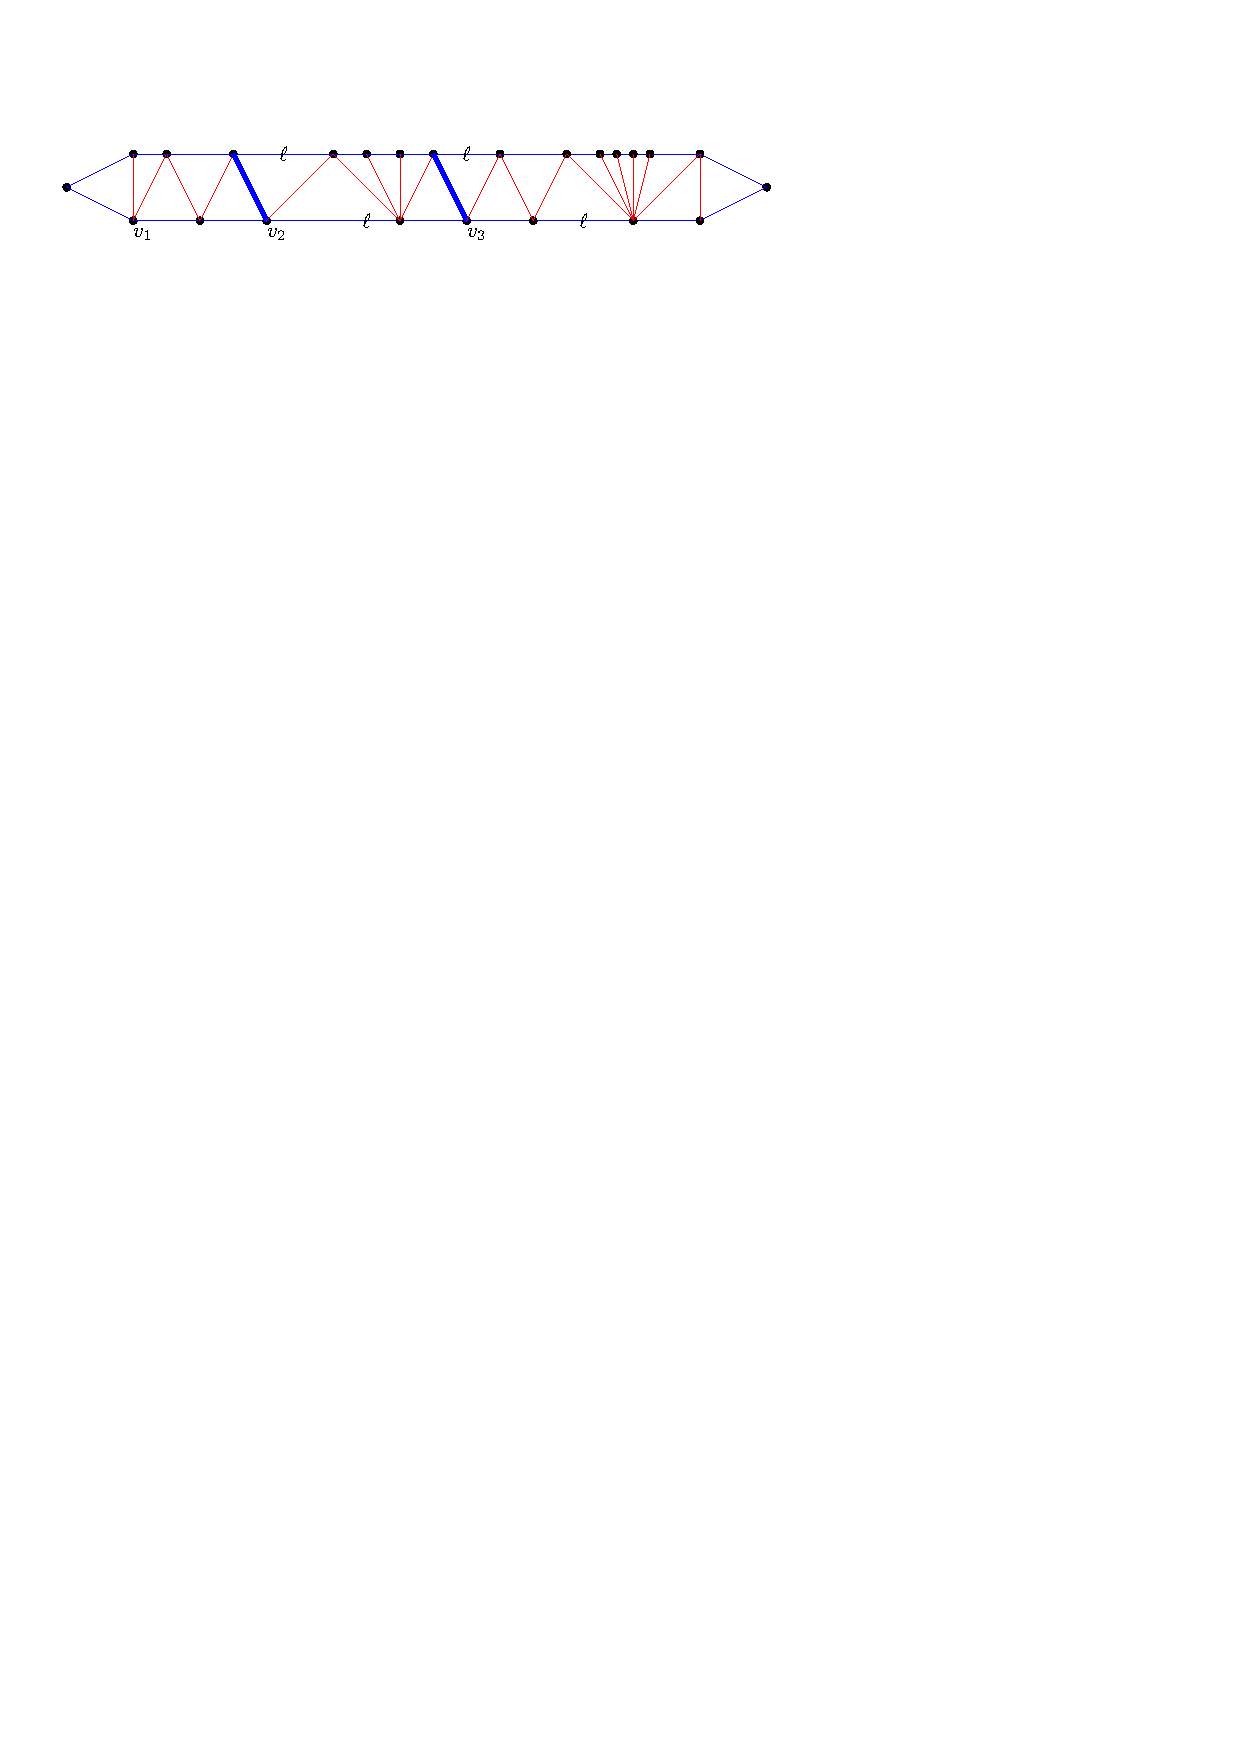
\includegraphics[scale=1]{blueFaceSubdivision/img/sampleExecution}
  \caption{Sample execution of the algorithm}
  \label{fig:subdiv:sampleExecution}
\end{figure}


\subsection{Face starting with a large topfan}
\fxnote{It might be $d-1$ in worst case}
The same algorithm as in Lemma \ref{lm:subdiv:withoutTopfan} after skipping the first topfan instead of the first edge finds us a finds us an edge keeping this face as at most a $ d - 3 +3 = d$-sided face. A sample worst case scenario is given in Figure \ref{fig:subdiv:worstCaseWithTopFan}.

\begin{figure}[h]
  \centering
  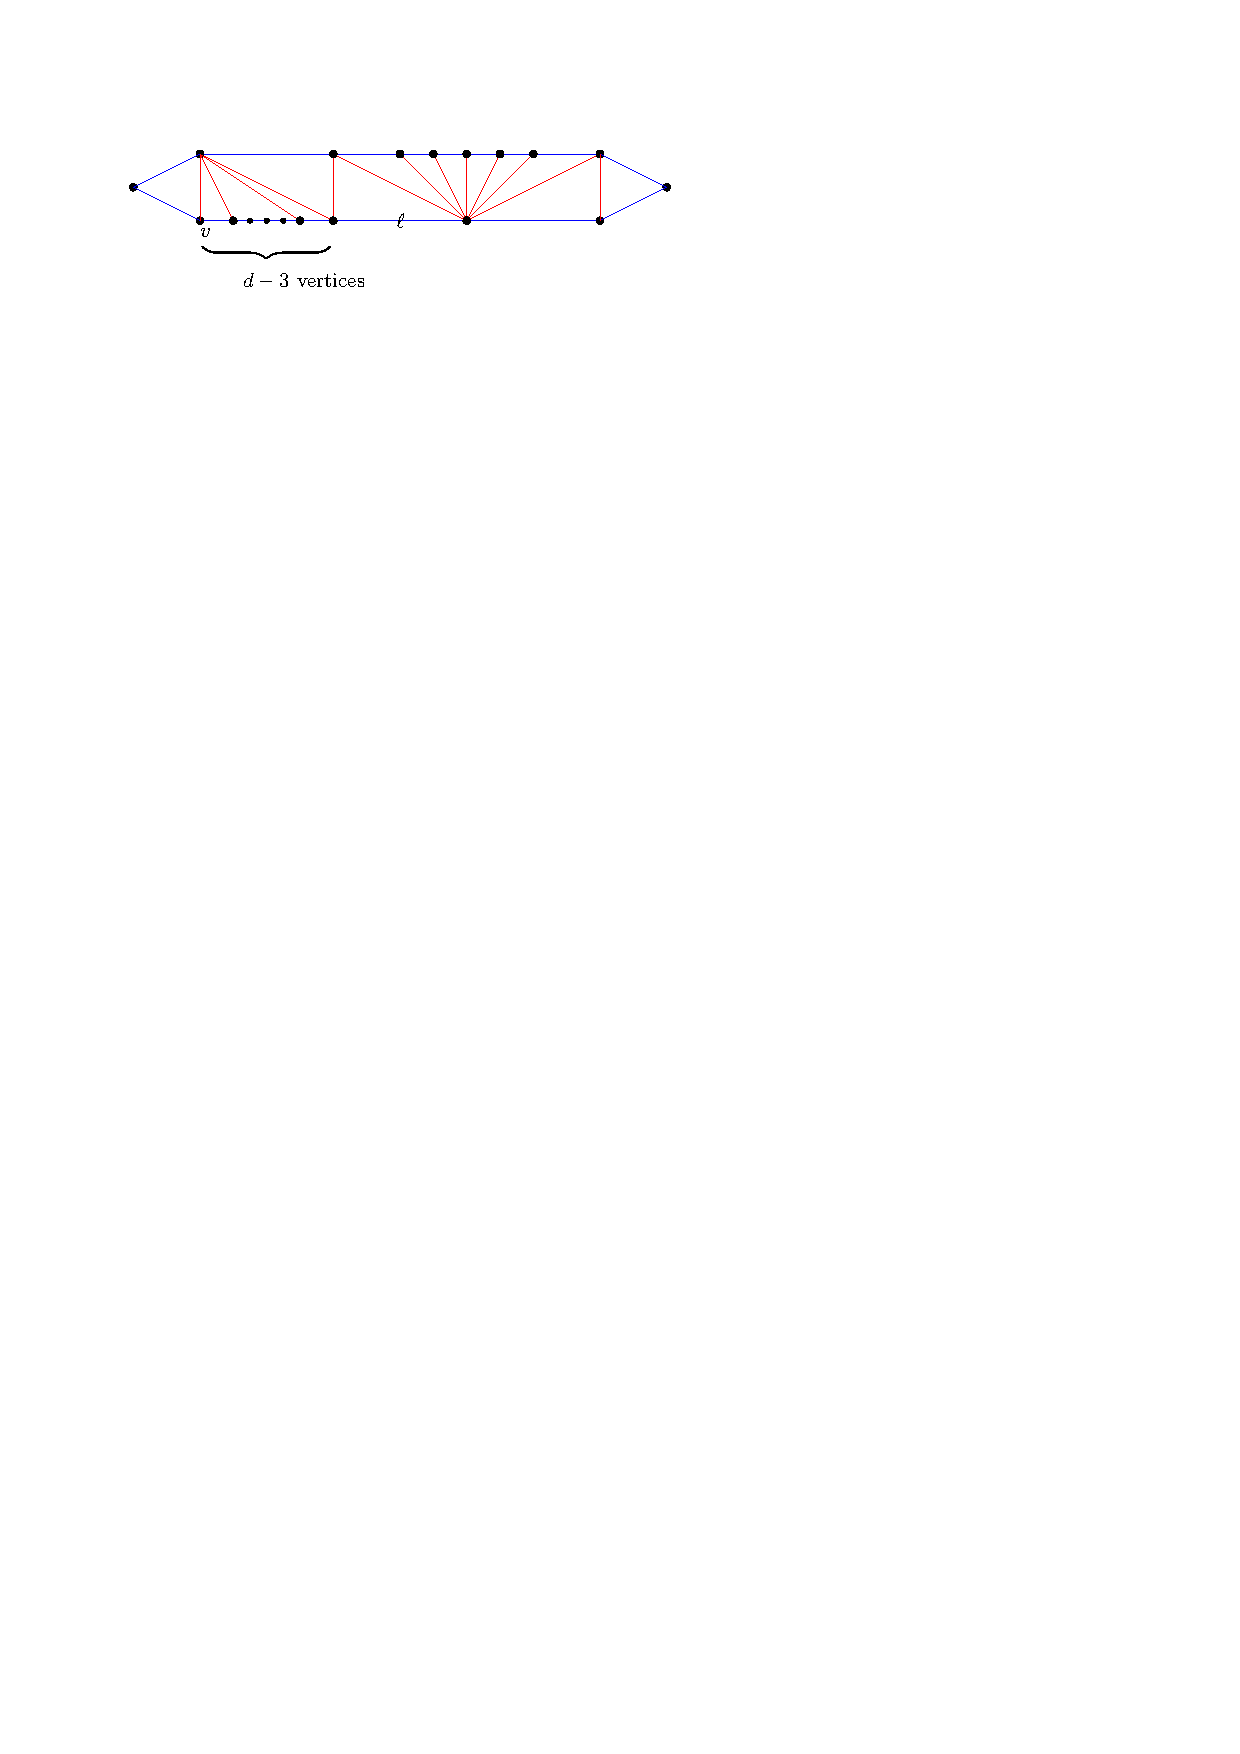
\includegraphics[scale=1]{blueFaceSubdivision/img/worstCaseWithTopFan}
  \caption{A worst case blue face. We don't flip any edge in this face.}
  \label{fig:subdiv:worstCaseWithTopFan}
\end{figure}


\subsection{Face encountering a larger topfan}
If we have a large topfan in the middle of the face then above the left outer edge of this topfan we can't have another topfan that failed to flip its left outer edges by Lemma \ref{lm:sweep:NoTwoSplitsAboveEachOther}.

This means we can use the following rule: we flip the first edge of a topfan even above a loaded edge. And still make only chains of at most $2$ $Z$'s.


\subsection{General conclusion}
\begin{lemma}
  \label{lm:subdiv:2chaindedZ}
  Two chained $Z$'s give at worst a $d-1$-sided face
\end{lemma}
\begin{proof}
  Before creating the $Z$'s in this section the \rel was vertically onesided. This also implies that  any $Z$ we now create can have at most one large merge/split fan on the top and one large merg/split fan on the bottom.

  So for two $Z$'s we have at most three large merge or split fans. Hence we have at most off one of these. Let's say without loss of generality that we have only one large merge. Then the left boundary edge of this face has at most $d-3 + 1 +1 =d-1$ vertices not counting the split and merge vertex of the red face.
\end{proof}

\begin{thrm}
  \label{th:final}
  We have a d-sided REL
\end{thrm}

\begin{proof}
  By construction a blue faces are $d$-sided. We have chained at most two $Z's$ so all red face contain at most two blue $Z$. So red faces are $d-1$-sided by Lemma \ref{lm:subdiv:2chaindedZ}.
\end{proof}


%%!TEX root = ../thesis.tex

\section{Example execution} %And worst case scenearios
\label{s:ex}
\thispagestyle{plain}

%\subsection{A small example}
On the four next pages we will give an example execution of our algorithm on a fairly simple graph.
We hope this helps the reader to get some intuition of how the algorithm operates. We consider the graph given in Figure~\ref{fig:ex:simple:1} this graph has as highest degree vertices several vertices of degree 6. Our algorithm should thus give at least a $5$-sided layout, but it actually gives a $2$-sided layout in this case.

The application of the algorithm to the graph is straightforward. Figures \ref{fig:ex:simple:1} to \ref{fig:ex:simple:7} are steps in the sweepline algorithm. This graph does not have any blue $Z$'s or topfans so we can skip these steps of the algorithm.
Then finally the subdivision of large red faces happen in Figure \ref{fig:ex:simple:8}.

In the captions of the subfigures of Figure~\ref{fig:ex:simple} more details about each step can be found.

\begin{figure}
    \centering
    \begin{subfigure}[b]{.9 \textwidth}
      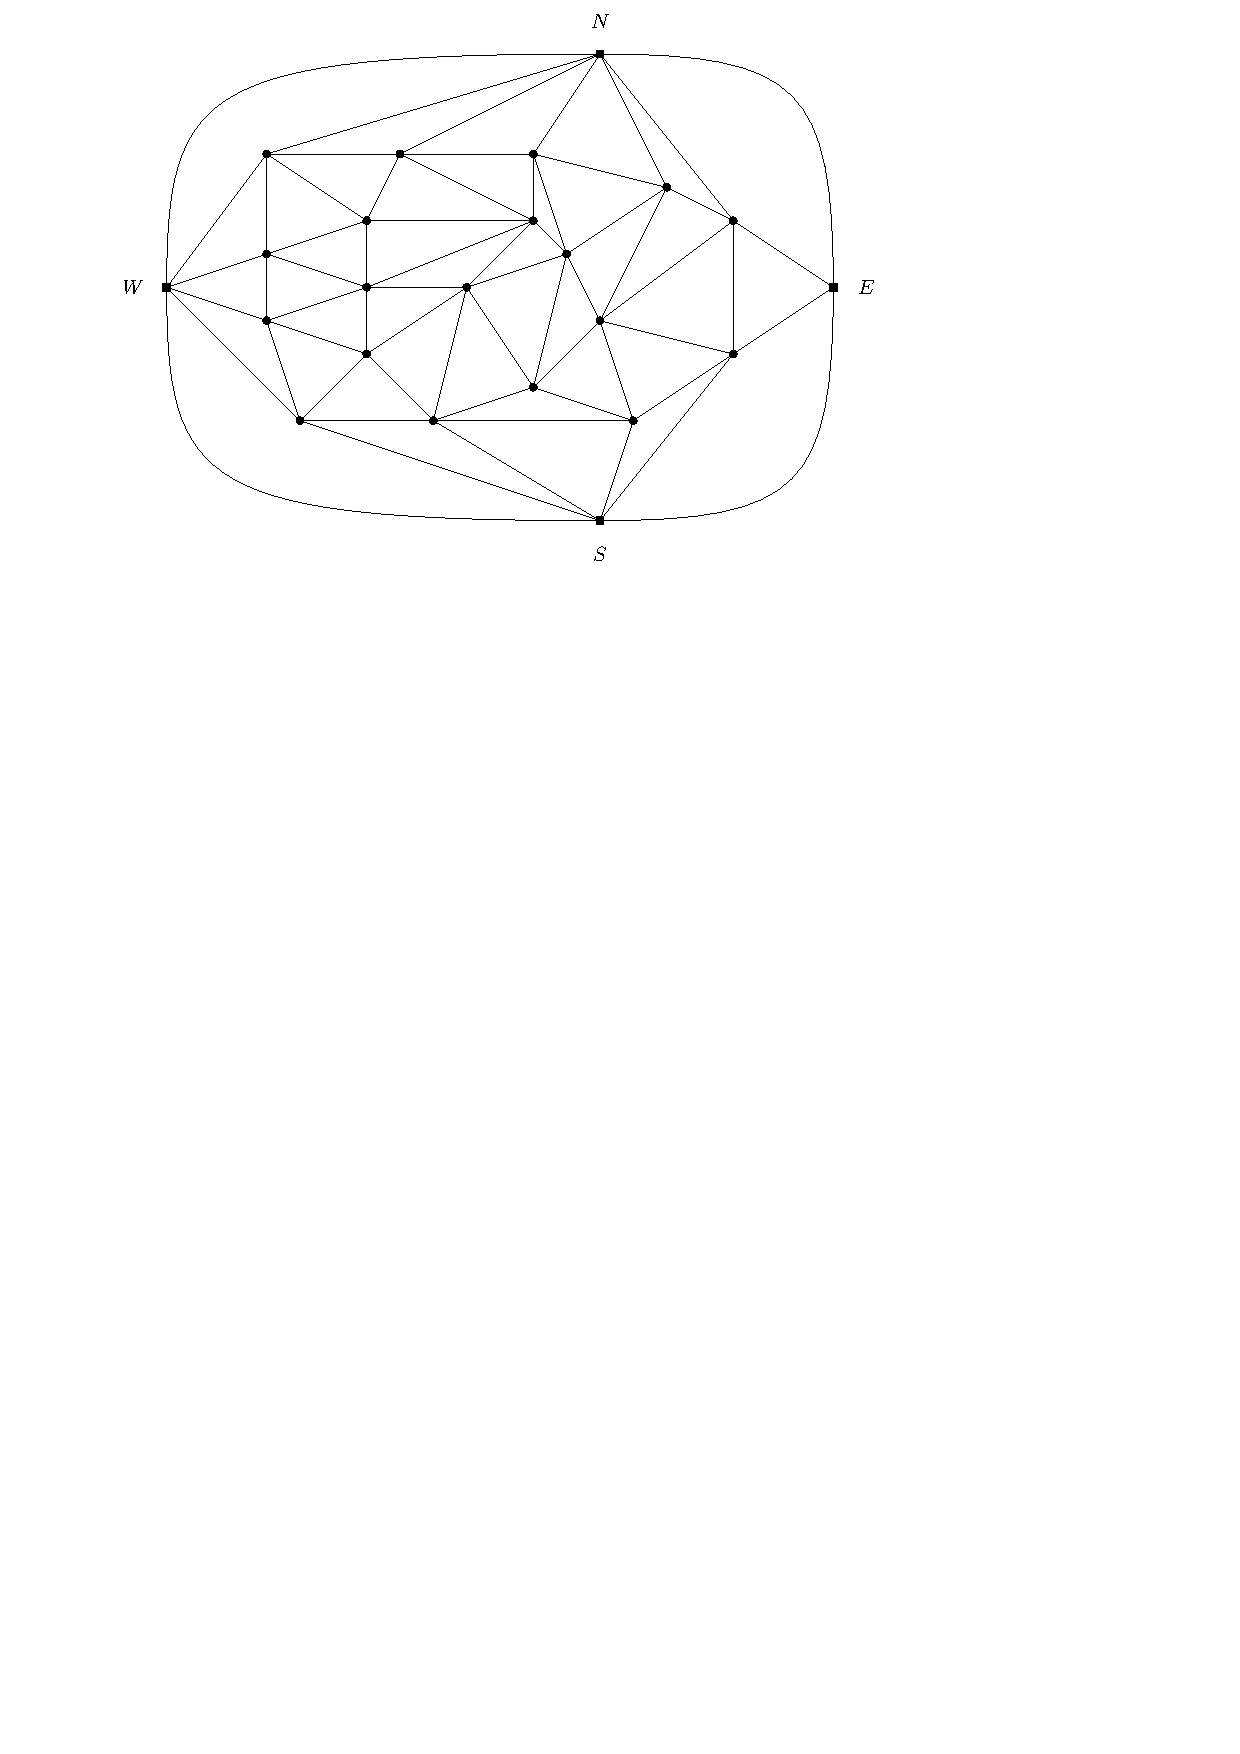
\includegraphics[width=\textwidth]{examples/img/smallExample/smallExample-1}
      \caption{The graph upon which we will execute the algorithm.}
      \label{fig:ex:simple:1}
    \end{subfigure}
    ~
    \begin{subfigure}[b]{.9 \textwidth}
      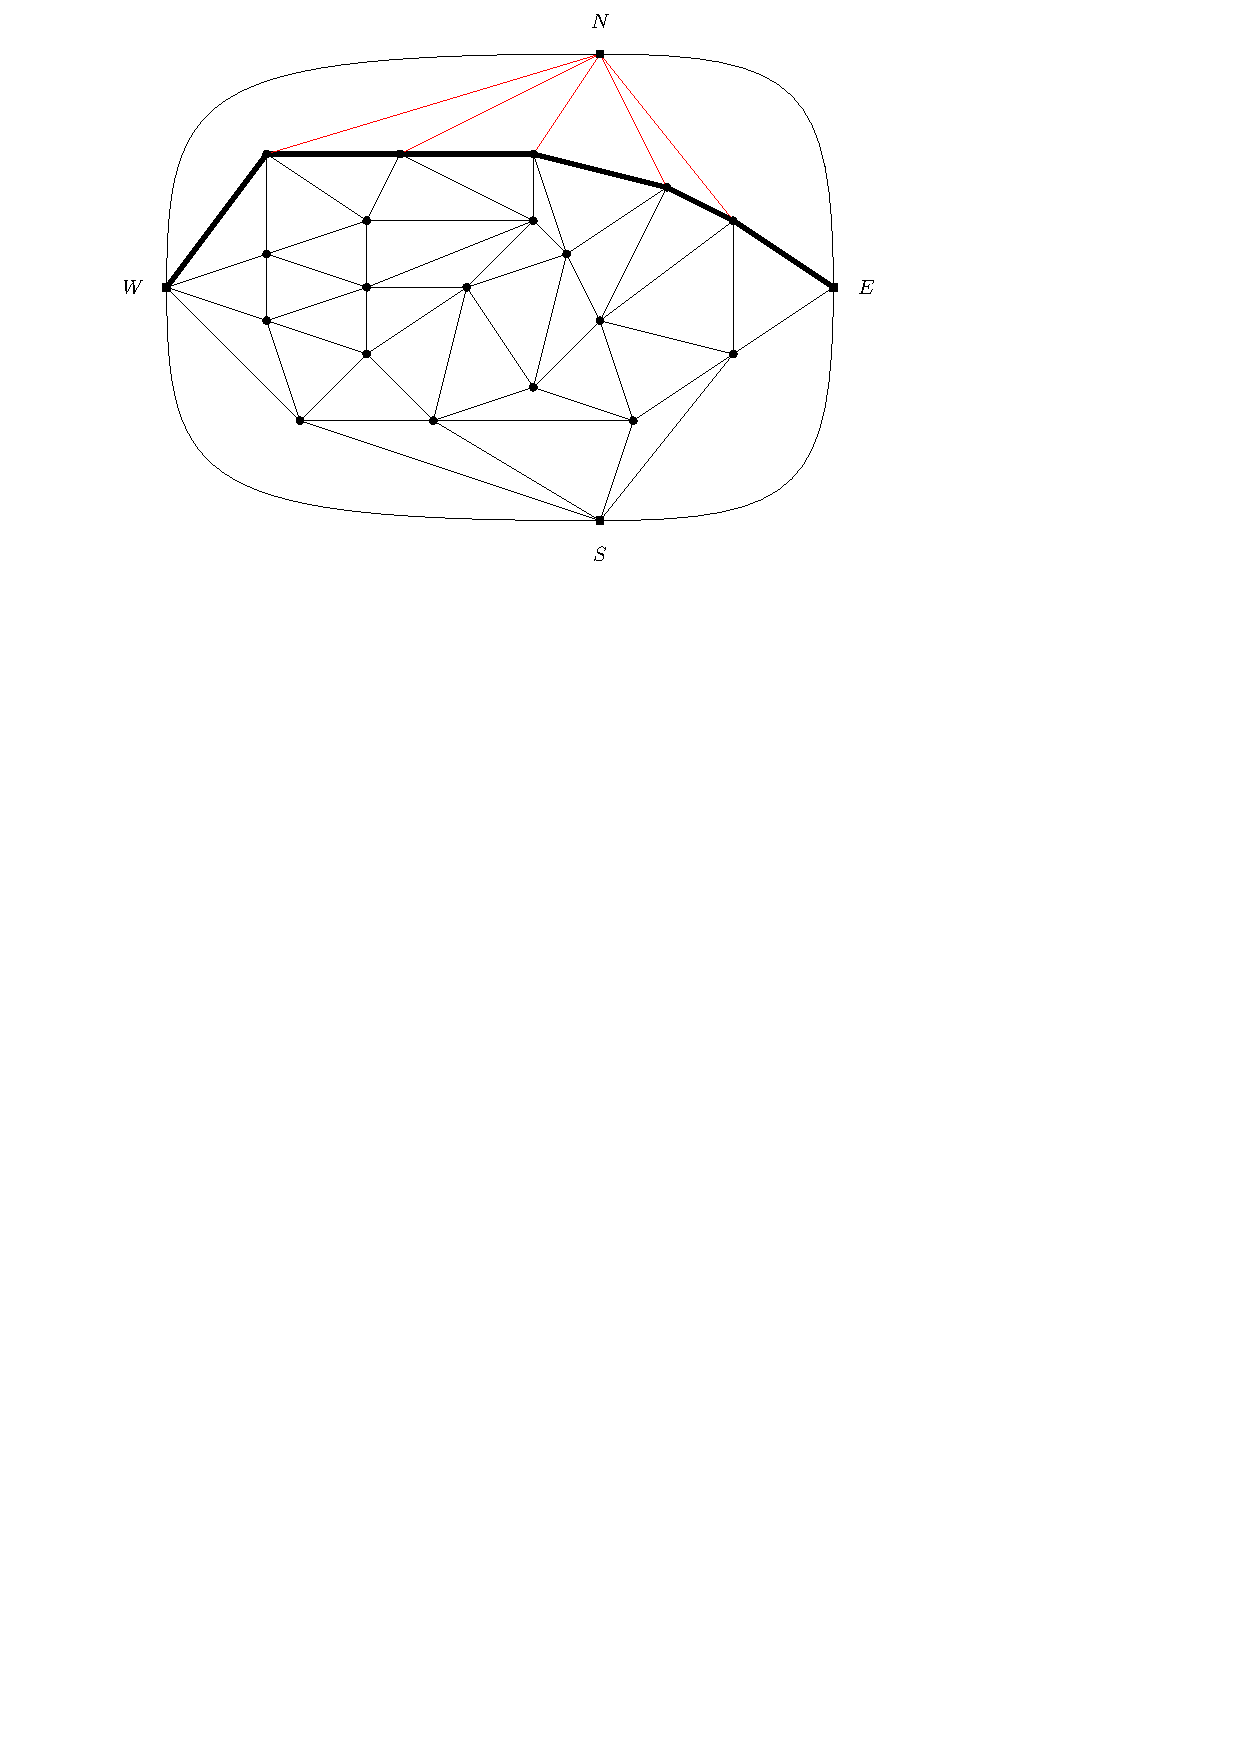
\includegraphics[width=\textwidth]{examples/img/smallExample/smallExample-2}
      \caption{The initial sweepcycle.}
      \label{fig:ex:simple:2}
    \end{subfigure}
    \label{fig:ex:vert}
    \caption{The steps of the algorithm.}
\end{figure}

\begin{figure}
    \centering
    \ContinuedFloat
    \begin{subfigure}[b]{.9 \textwidth}
      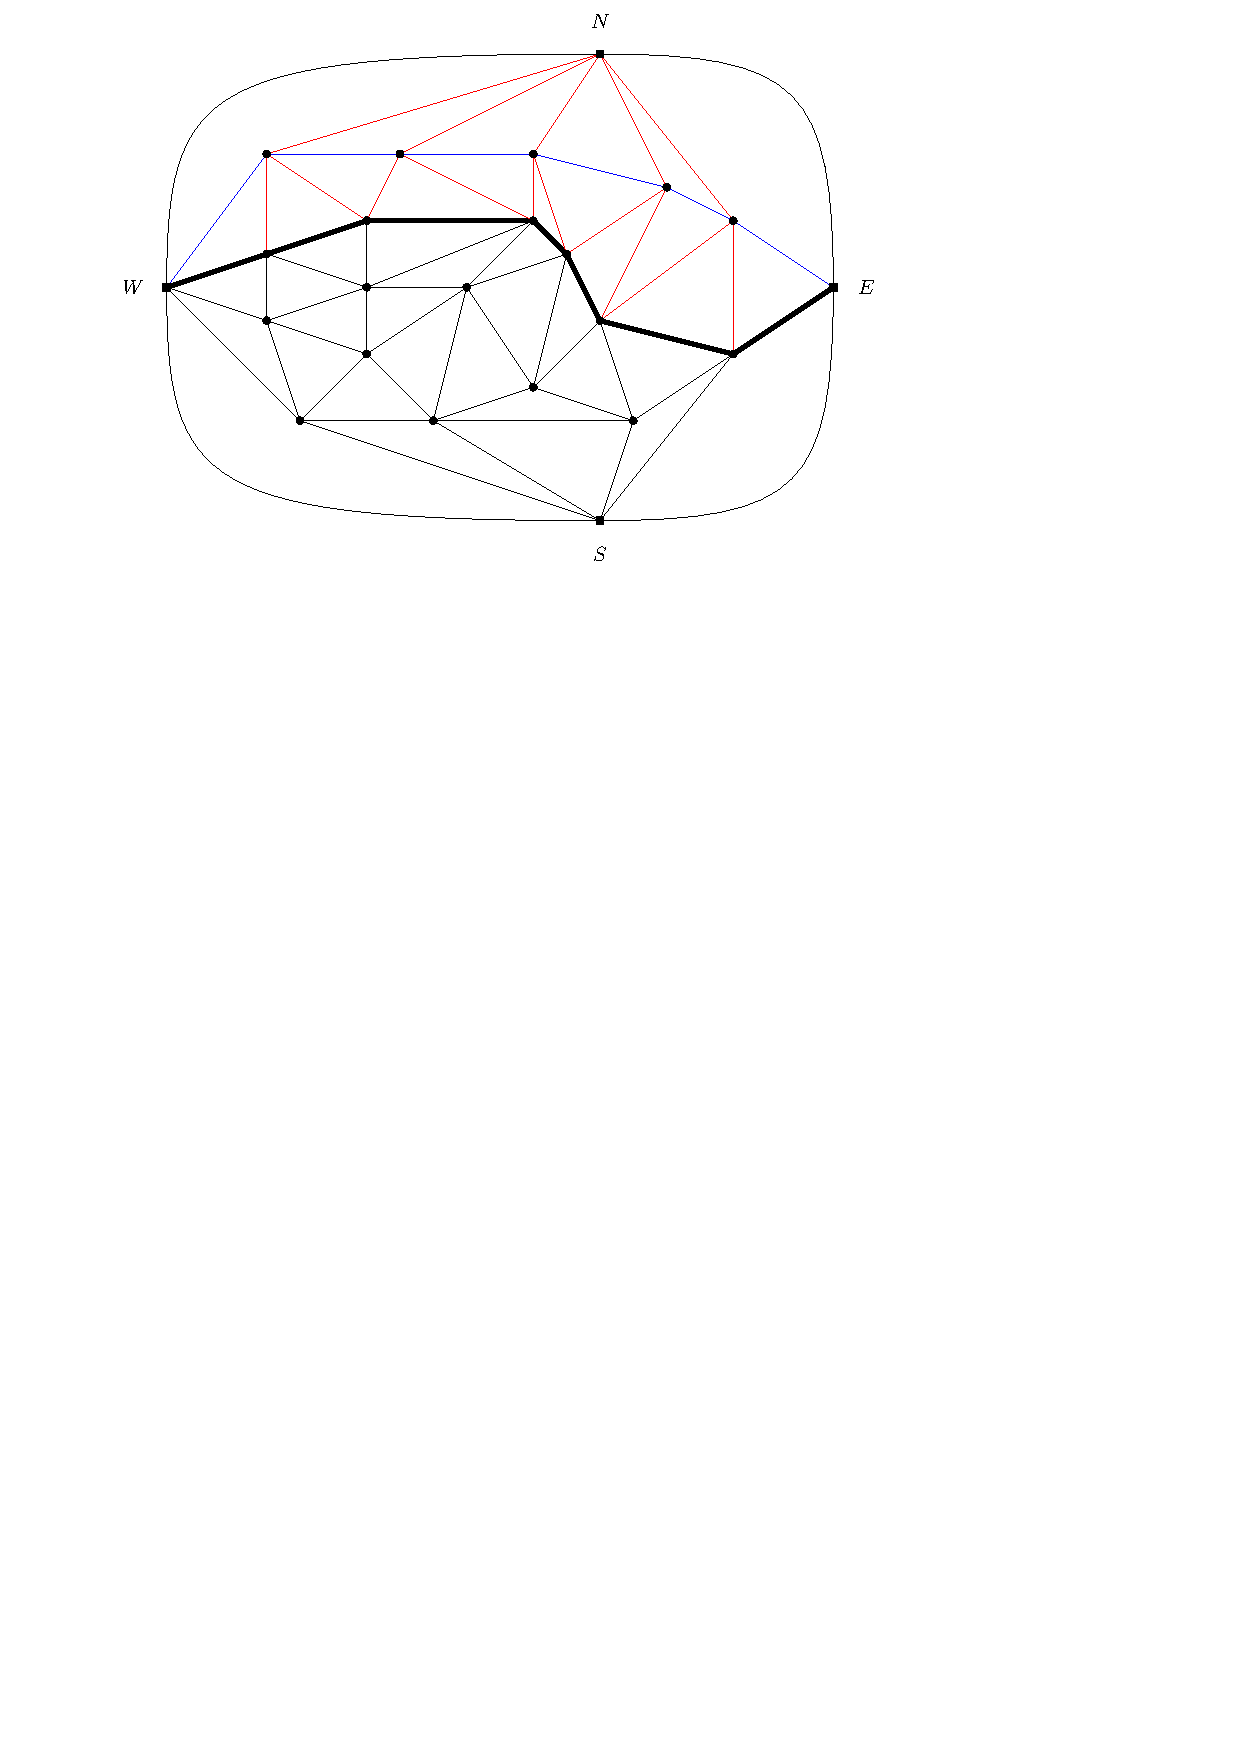
\includegraphics[width=\textwidth]{examples/img/smallExample/smallExample-3}
      \caption{Advancing by one update of the sweepcycle.}
      \label{fig:ex:simple:3}
    \end{subfigure}
    ~
    \begin{subfigure}[b]{.9 \textwidth}
      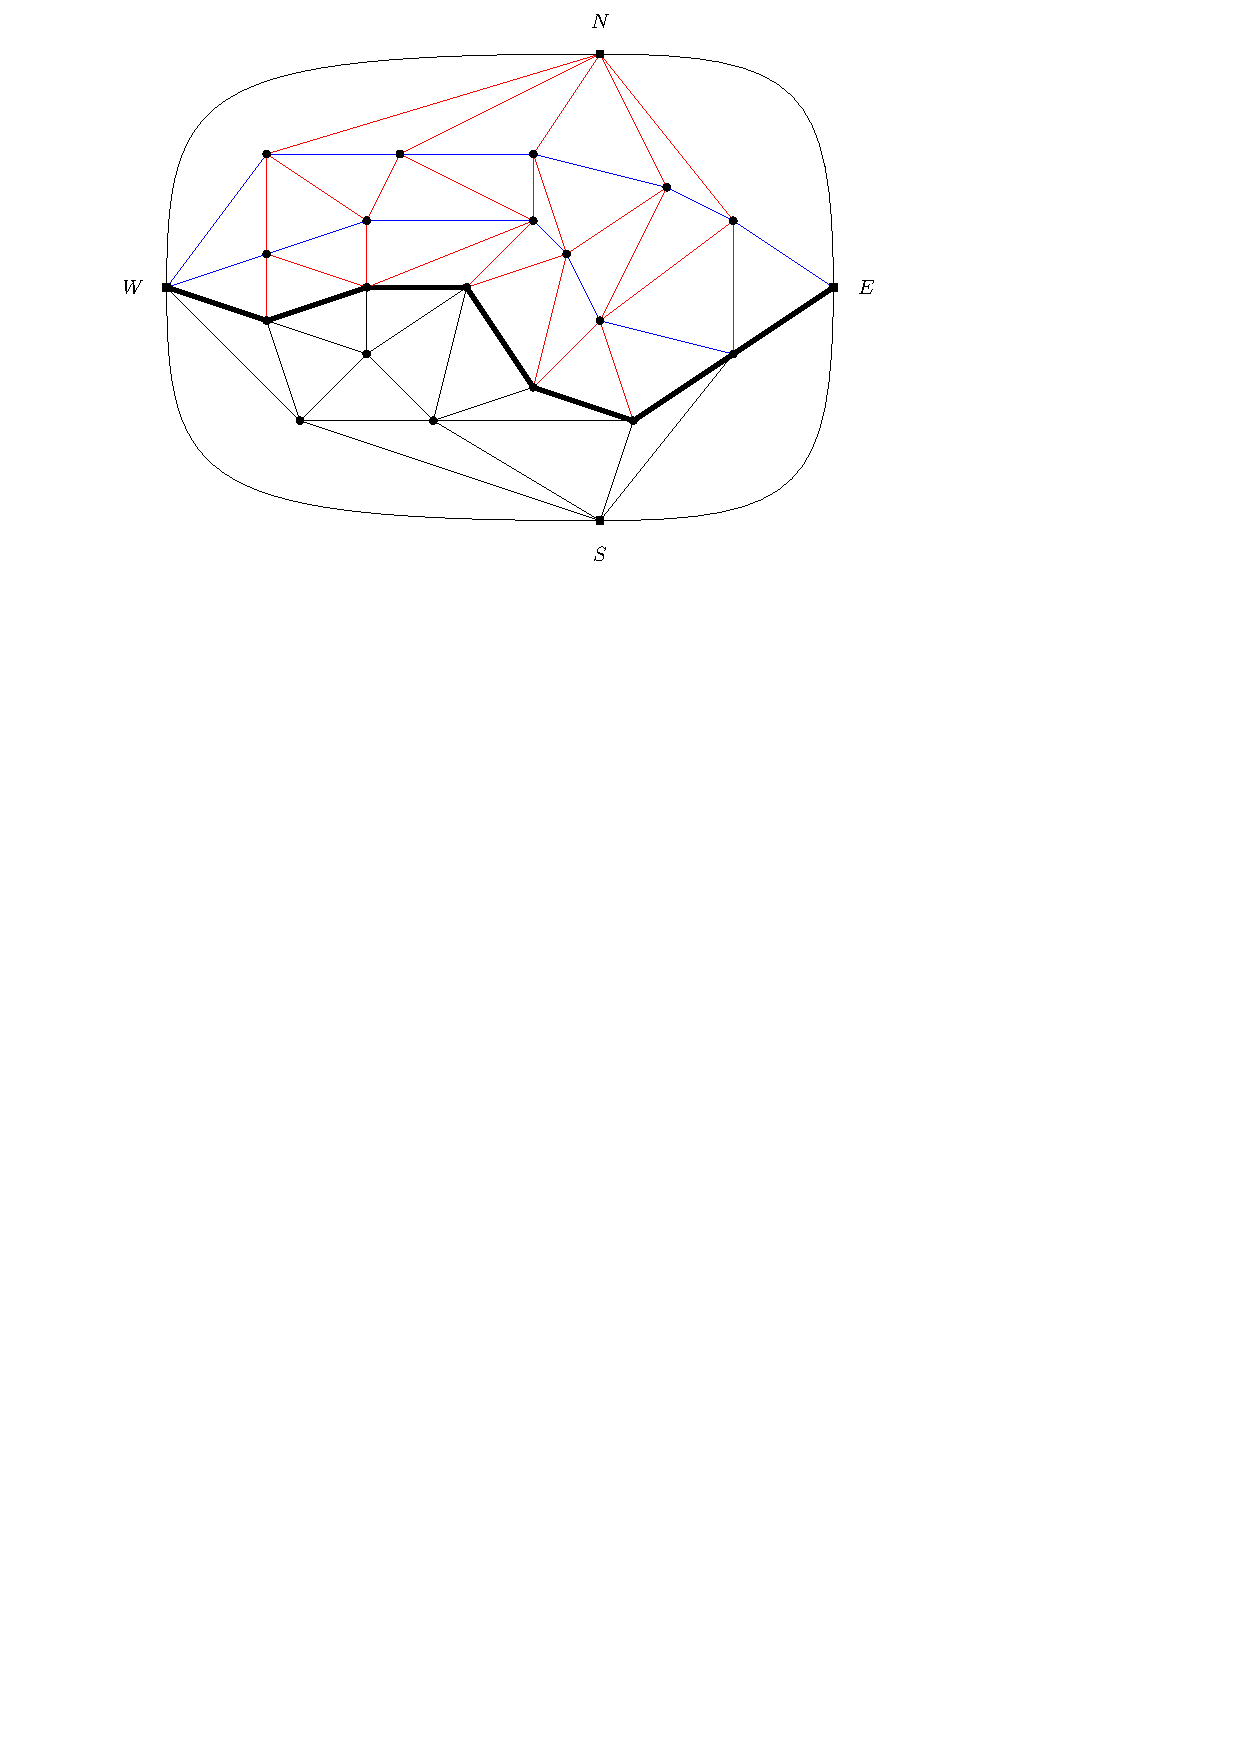
\includegraphics[width=\textwidth]{examples/img/smallExample/smallExample-4}
      \caption{Another update step.}
      \label{fig:ex:simple:4}
    \end{subfigure}
    \caption{The steps of the algorithm.}
\end{figure}

\begin{figure}
    \centering
    \ContinuedFloat
    \begin{subfigure}[b]{.9 \textwidth}
      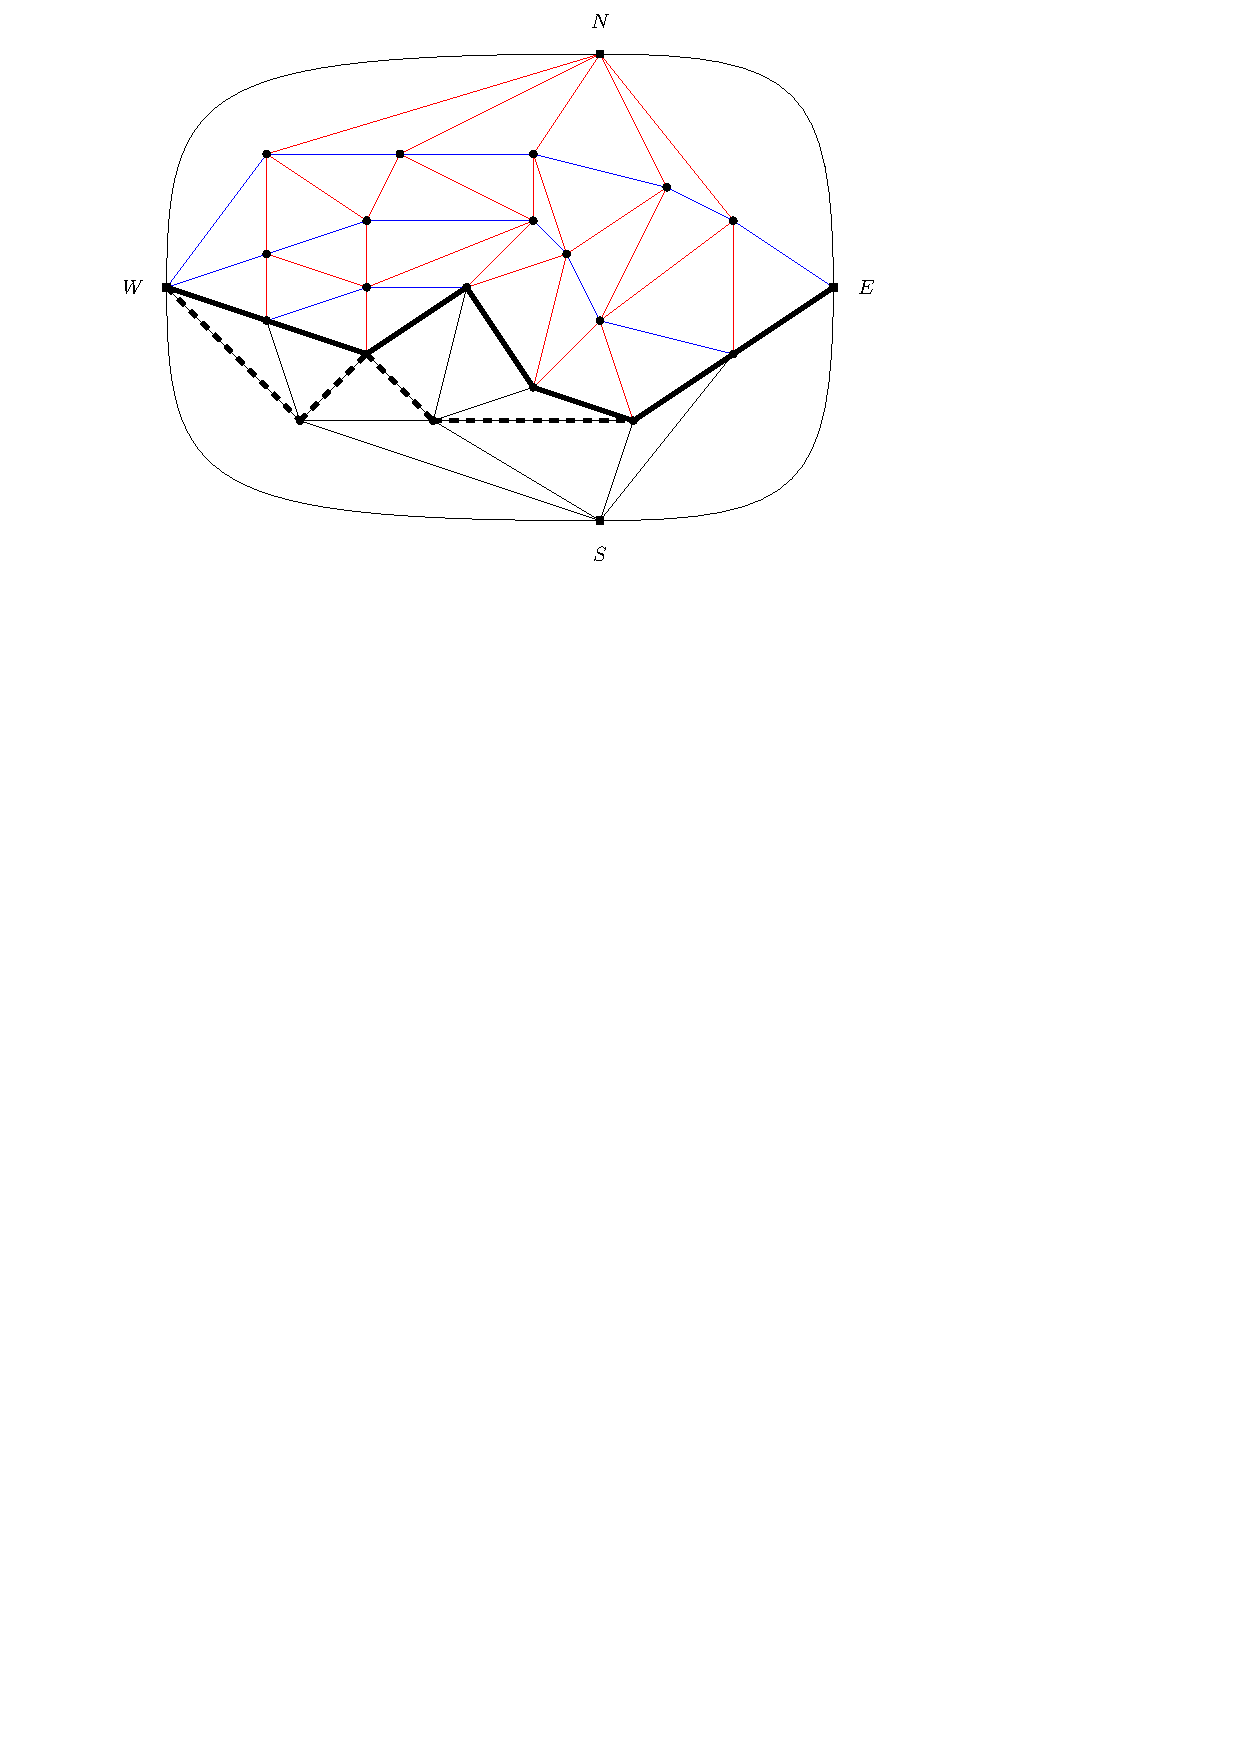
\includegraphics[width=\textwidth]{examples/img/smallExample/smallExample-5}
      \caption{This update the candidate path (dashed) had a chord leading to this smaller update.}
      \label{fig:ex:simple:5}
    \end{subfigure}
    ~
    \begin{subfigure}[b]{.9 \textwidth}
      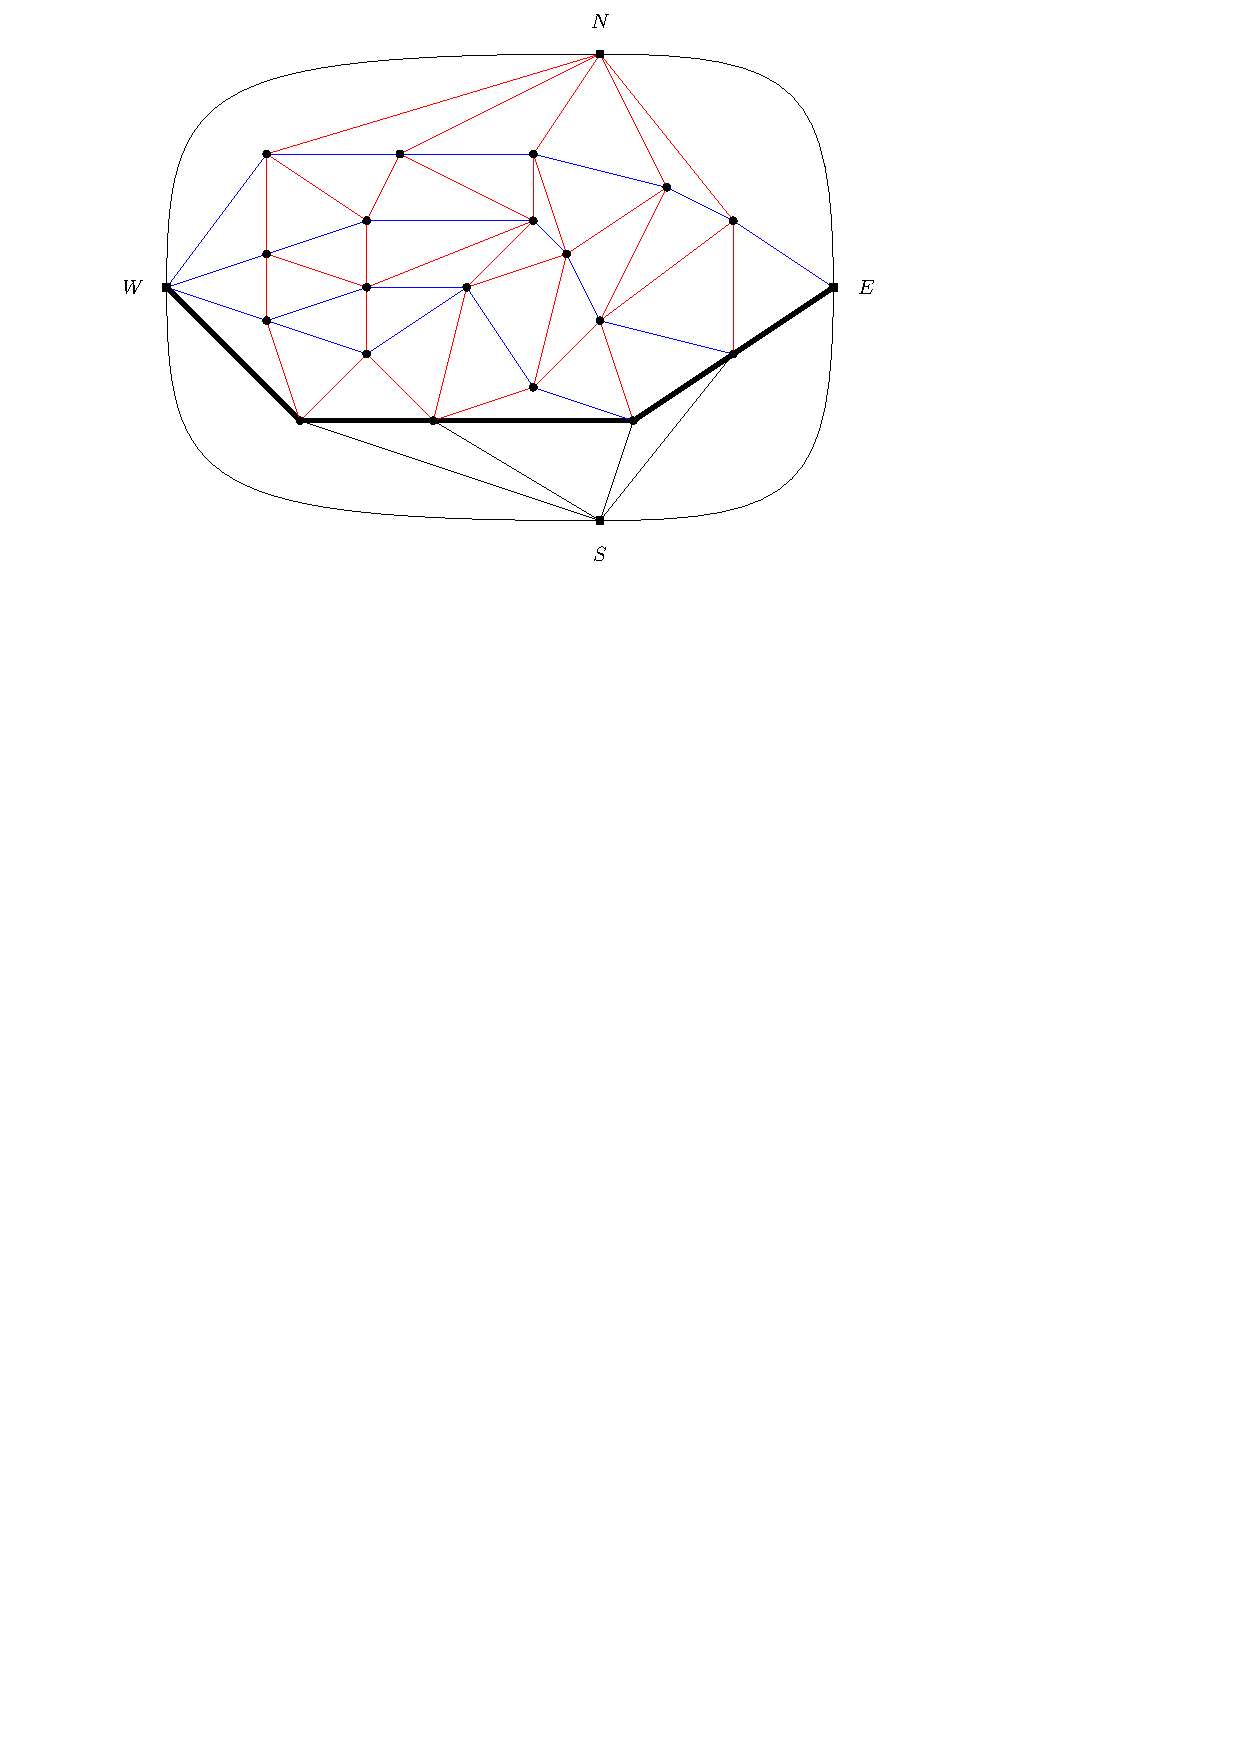
\includegraphics[width=\textwidth]{examples/img/smallExample/smallExample-6}
      \caption{Another update step. This time again without violating chords.}
      \label{fig:ex:simple:6}
    \end{subfigure}
    \caption{The steps of the algorithm.}
\end{figure}

\begin{figure}
    \centering
    \ContinuedFloat
    \begin{subfigure}[b]{.9 \textwidth}
      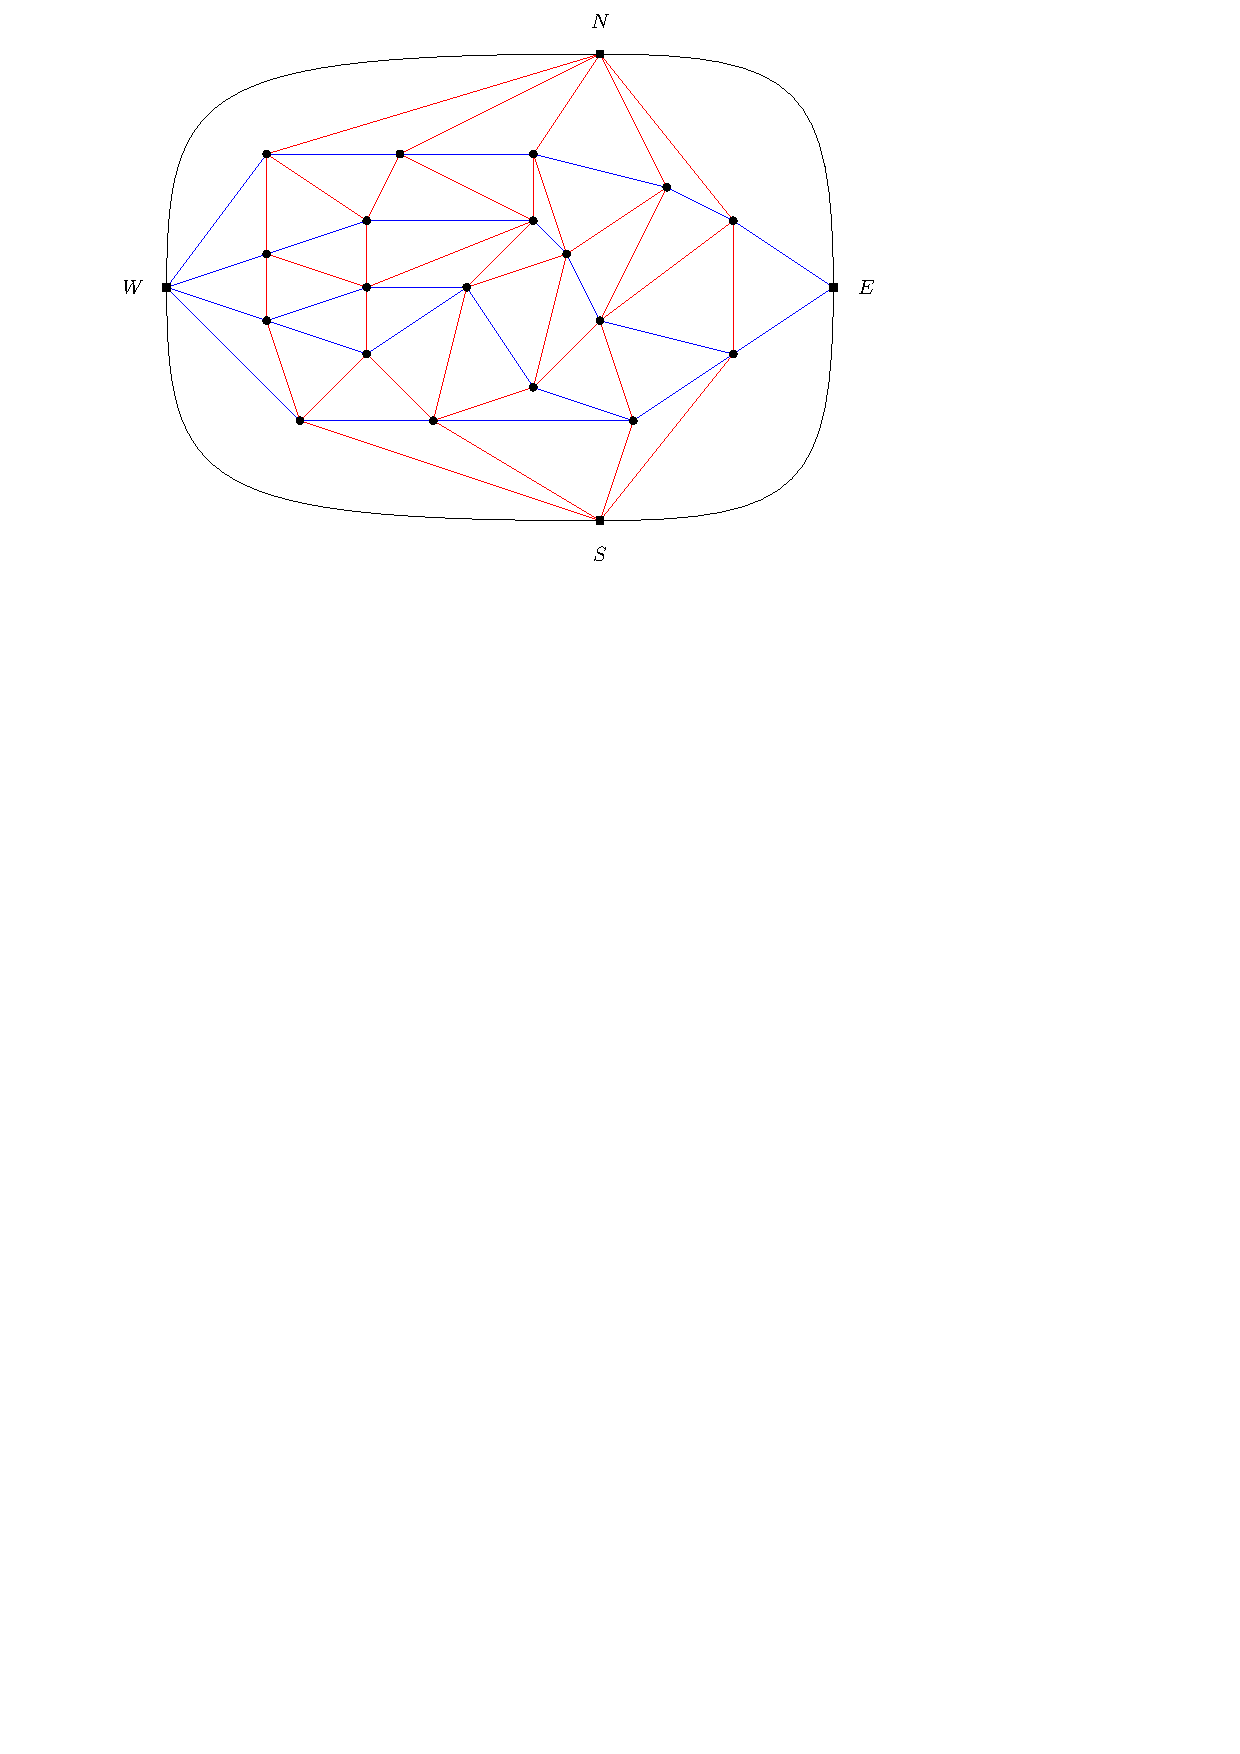
\includegraphics[width=\textwidth]{examples/img/smallExample/smallExample-7}
      \caption{Terminating the sweepcycle step of the algorithm.}
      \label{fig:ex:simple:7}
    \end{subfigure}
    ~
    \begin{subfigure}[b]{.9 \textwidth}
      \includegraphics[width=\textwidth]{examples/img/smallExample/smallExample-8}
      \caption{The flips we make during blue face subdivision.}
      \label{fig:ex:simple:8}
    \end{subfigure}
  \caption{The steps of the algorithm.}
  \label{fig:ex:simple}

\end{figure}




%\subsection{A example containing a large red face}
%
%Consider the graph given in Figure~\ref{fig:ex:vert:graph} this graph has as highest degree %vertices two vertices of degree 12. We show how the proposed algorithm handles this graph.
%
%The way in which the algorithm handles this graph is far from ideal leading to a 10-sided face. %While the provided upperbound would lead to (at worst) a 11-sided \fxnote{11 or 12?} face. %Furthermore the approach in this graph is scaleabale as is shown in Figure~\ref{some figure TODO %Show where to scale using dashed lines etc..}
%
%\begin{figure}[h]
%  \centering
%  \includegraphics[width=\textwidth]{examples/img/vertWorstCase/graph}
%  \caption{}
%  \label{fig:ex:vert:graph}
%\end{figure}
%
%The application of the algorithm to this graph is straightforward. Figures \ref{fig:ex:vert:sweep1} %to \ref{fig:ex:vert:sweepfinal} are steps in the sweepline algorithm. This graph does not permit %any topfanflips since all large topfans are either incident to a pole or starting above a split %vertex. \fxnote{In a sense a pole is a splitvertex}
%Then finally the subdivision of large red faces happen in Figures \ref{fig:ex:vert:subdiv1} and %\ref{fig:ex:vert:subdivfinal}.
%
%In the captions of the subfigures of Figure~\ref{fig:ex:vert} more details about each step can be %found.
%
%
%\begin{figure}
%    \centering
%    \begin{subfigure}[b]{.9 \textwidth}
%      \includegraphics[width=\textwidth]{examples/img/vertWorstCase/sweep1}
%      \caption{The initial sweepcycle.}
%      \label{fig:ex:vert:sweep1}
%    \end{subfigure}
%    ~
%    \begin{subfigure}[b]{.9 \textwidth}
%      \includegraphics[width=\textwidth]{examples/img/vertWorstCase/sweep2}
%      \caption{Advancing by one update of the sweepcycle.}
%      \label{fig:ex:vert:sweep2}
%    \end{subfigure}
%    \label{fig:ex:vert}
%    \caption{The steps of the algorithm.}
%\end{figure}
%
%\begin{figure}
%    \ContinuedFloat
%    \begin{subfigure}[b]{.9 \textwidth}
%      \includegraphics[width=\textwidth]{examples/img/vertWorstCase/sweep3}
%      \caption{This update the candidate path had a chord leading to this smaller update step.}
%      \label{fig:ex:vert:sweep3}
%    \end{subfigure}
%    ~
%    \begin{subfigure}[b]{.9 \textwidth}
%      \includegraphics[width=\textwidth]{examples/img/vertWorstCase/sweep4}
%      \caption{Several similar update steps combined into one figure.}
%      \label{fig:ex:vert:sweep4}
%    \end{subfigure}
%    \caption{The steps of the algorithm.}
%\end{figure}
%
%\begin{figure}
%    \ContinuedFloat
%    \begin{subfigure}[b]{.9 \textwidth}
%      \includegraphics[width=\textwidth]{examples/img/vertWorstCase/sweep5}
%      \caption{An update step, this time without violating chords.}
%      \label{fig:ex:vert:sweep5}
%    \end{subfigure}
%    ~
%    \begin{subfigure}[b]{.9 \textwidth}
%      \includegraphics[width=\textwidth]{examples/img/vertWorstCase/sweep6}
%      \caption{Another update step. Note that the original candidate path would have a polebound %2-chord with the edge $\pE \pS$.}
%      \label{fig:ex:vert:sweep6}
%    \end{subfigure}
%    \caption{The steps of the algorithm.}
%\end{figure}
%
%\begin{figure}
%    \ContinuedFloat
%    \begin{subfigure}[b]{.9 \textwidth}
%      \includegraphics[width=\textwidth]{examples/img/vertWorstCase/sweep7}
%      \caption{}
%      \label{fig:ex:vert:sweep7}
%    \end{subfigure}
%    ~
%    \begin{subfigure}[b]{.9 \textwidth}
%      \includegraphics[width=\textwidth]{examples/img/vertWorstCase/sweep8}
%      \caption{}
%      \label{fig:ex:vert:sweep8}
%    \end{subfigure}
%  \caption{The steps of the algorithm.}
%  \label{}
%
%\end{figure}
%
%
%
%\begin{figure}
%    \ContinuedFloat
%    \begin{subfigure}[b]{.9 \textwidth}
%      \includegraphics[width=\textwidth]{examples/img/vertWorstCase/sweepfinal}
%      \caption{}
%      \label{fig:ex:vert:sweepfinal}
%    \end{subfigure}
%    ~
%    \begin{subfigure}[b]{.9 \textwidth}
%      \includegraphics[width=\textwidth]{examples/img/vertWorstCase/subdiv1}
%      \caption{}
%      \label{fig:ex:vert:subdiv1}
%    \end{subfigure}
%  \caption{The steps of the algorithm.}
%  \label{}
%\end{figure}
%
%
%
%\begin{figure}
%    \ContinuedFloat
%    \begin{subfigure}[b]{.9 \textwidth}
%      \includegraphics[width=\textwidth]{examples/img/vertWorstCase/subdivfinal}
%      \caption{}
%      \label{fig:ex:vert:subdivfinal}
%    \end{subfigure}
%  \caption{The steps of the algorithm.}
%  \label{}
%\end{figure}
%


%\section{Running time analysis}
\thispagestyle{plain}
%\section{Conclusion}
\thispagestyle{plain}


\listoffixmes

%%!TEX root = ../thesis.tex

% All results in this chapter hold

\section{Appendix: Additional results on triangulations and triangulations of the k-gon}

\subsection{Connectedness of triangulations}
  Let us first note that any maximally planar graph is $2$-connected. Suppose there is a cutvertex, then surly we can add an edge between the components found after removing this cutvertex.

  \begin{thrm}
    Any plane triangulation $T$ is $3$-connected.
    \label{th:plTri3Connected}
  \end{thrm}

  \begin{proof}
    Suppose that $T$ is not $3$-connected. Then there must be a $2$-cutset $S$, given by the vertices $x$ and $y$. Removing this cutset splits the graph into at least two connected components $C_i$ with all components incident to all cutvertices. Since otherwise we would have found a $1$-cutset.

    Because $S$ is a cutset, there can't be any edges connecting $C_1$ and $C_2$. But then the edge $xy$ should be separating the $2$ components on both sides. This is impossible since we can only draw this edge once.
    %\fxnote{We could add a figure to make this more clear}
  \end{proof}

  \begin{defi}[Irreducible triangulation]
  We call a triangulation irreducible if it has no separating triangles
  \end{defi}

  \fxnote{It is called irreducible because there is a reduction that works on separating triangles. We might show this reduction. predraft-2}

  \begin{thrm}
  Any irreducible plane triangulation $T$ is $4$-connected.
  \end{thrm}

  \begin{proof}
    Note that any plane triangulation is $3$-connected by Theorem \ref{th:plTri3Connected}.

    Suppose that $T$ is not $4$-connected. Then there must be some $3$-cutset (since it is $3$-connected) let us denote the vertices of this cutset by $x, y$ and $z$. Removing this cutset splits the graph into at least two connected components $C_i$ and all components are incident to all cutvertices otherwise we would have found a $2$- or $1$-cutset.

    However, now $xy$ must be an edge in the triangulation $T$ otherwise the graph is not maximal planar (There can't be an edge incident to both $C_1$ and $C_2$ because that would negate $x, y ,z$ being a cutset.). In the same way $yz$ and $xz$ are edges of $T$. But then $xyz$ is a separating triangle. This is an contradiction and thus $T$ is $4$-connected
  \end{proof}

\subsection{Connectedness of triangulations of the $k$-gon}
  \begin{defi}[Irreducible triangulation of the $k$-gon]
  We call a triangulation of the $k$-gon irreducible if it has no separating triangles.
  \end{defi}


  Note that triangulation of the $n$-gon $n\geq 4$ is not maximally planar and thus not plane triangulation.

  The \emph{completion} of a triangulation of the $k$-gon $G = (V, E)$. Is the graph $G'= (V', E')$ with vertex set $V' = V \cup \braces{s}$ and edge set $E' = E \cup \braces{ sv | v \text{ is a outer vertex}}$

  The completion is plane triangulation.  %Q does this stament need proof?
  Since the interior of the outer cycle of $G$ always consisted of faces of degree 3. The exterior of the outer cycle consisted of one face of degree $k$ (the outer face) but the completion has turned this into $k$ faces of degree $3$.

  \begin{thrm}
  A triangulation of the $k$-gon $G$ is $2$-connected.
  \end{thrm}
  \begin{proof}
  Suppose that $G$ has a cutvertex $v$. Then the set $\braces{s, v}$ is a $2$-cutset of the completion $G'$ of $G$. This however is in contradiction to Theorem \ref{th:plTri3Connected} stating that $G'$ is $3$-connected. Hence $G$ has no cutvertex and is thus $2$-connected.
  \end{proof}

  \begin{thrm}
    \label{th:triOfK3:VertexDisjointPaths}
    For every interior vertex $v$ of a triangulation of the $k$-gon $G$ is connected by at least $3$ vertex disjoint paths to different outer vertices.
  \end{thrm}
  \begin{proof}
  By Theorem \ref{th:plTri3Connected} the completion $G'$ of $G$ is $3$-connected. Hence there are 3 vertex-disjoint paths from $v$ to $s$. Since $v$ is on the interior and $s$ is on the exterior of the outer cycle $\C$ all these 3 paths cross the outer cycle at least once. These paths cross $\C$ for the first time in different vertices since they are vertex-disjoint. If we shorten the paths to their first crossing with $\C$ we obtain the $3$ paths in the theorem.
  \end{proof}

  \fxnote{We can sharpen this to $4$ if we have a irreducible triangulation of the $k$-gon with a chordfree outer cycle}

%%!TEX root = ../thesis.tex

\section{Appendix: Unused theorems}


\begin{thrm}
\label{th:irreducible and chordfree triangulation of the kgon is 3connected}
A irreducible triangulation $G$ of the $k$-gon with a chordfree outer cycle is $3$-connected.
\end{thrm}
\begin{proof}
  This proof has to be expanded.

  The completion $G'$ is a irreducible triangulation. Chordfree outer cycle is important, because a chord will form a separating triangle in $G'$.
\end{proof}

\begin{thrm}
  Any irreducible triangulation $T$ of the $4$-gon with $n \geq 5$ is $3$-connected.
\end{thrm}
\begin{proof}
  Let us name the four vertices of the outer cycle $a,b,c,d$, this cycle has at least one interior vertex $v$ since $n\geq 5$. The edges $ac$ and $bd$ can't exist since they would create a separating triangle containing $v$. hence the outer cycle is chordfree.
  Theorem \ref{th:irreducible and chordfree triangulation of the kgon is 3connected} then concludes the proof
\end{proof}


\begin{thrm}
  Every interior vertex of a triangulation of the $n$-gon has degree at least $3$.
\end{thrm}

\begin{proof}
  This follows directly from Theorem \ref{th:triOfK3:VertexDisjointPaths}. If a interior vertex would have a lower degree it can never have $3$ vertex disjoint paths to the outer cycle.
\end{proof}

%\begin{proof}
%Suppose a interior vertex $v$ has degree $1$ then clearly the face surrounding $v$ can't have degree $3$. Now suppose that an interior vertex $v$ has degree $2$. We then let $u$ and $w$ denote it's neighbours and $F$ and $F'$ the face incident to $v$. See also Figure \ref{fig:interiorVertexDegree3}. Then since $F$ and $F'$ are both interior faces they need to be off degree $3$ this implies that $uw$ is an edge for both faces. This is impossible and hence every interior vertex has at least degree $3$
%\end{proof}

%\begin{figure}[h!]
%\centering
%\includegraphics{prelim/img/interiorVertexDegree3.pdf}
%\caption{The notation as described in the proof \label{fig:interiorVertexDegree3}
%}
%\end{figure}

\subsection{Incomplete proofs}
\begin{thrm}[Existence of a eligible path]
\label{th:eligExistence}
When the algorithm's invariant (\ref{i:SWandSE} - \ref{i:last}) are satisfied and the cycle $\C$ is separating then there exist a \emph{eligible} internal path.
\end{thrm}
\begin{proof}
We will first show that there always exists an internal path $\P$. We will then show that a internal path can be found that satisfies conditions $(E1) - (E4)$.

In the proof we will often use that a

Let us first note that if the cycle $C$ is separating (i.e has a non-empty interior), there is at least one interior vertex $v$. Since the triangulation of a $n$-gon is $2$-connected there are two ways to go from $v$ to (say) $S_r$. Hence there is an internal path $\P_0$.
%TODO this is not true, luckily we can use the connections to cyle lemma

If this path does not satisfy \ref{e:noS} we can use the following construction. The other vertex where $P_0$ intersects $\C$ is not $S_r$. Let us call this vertex $x$ and it's neighbor on the path $y$. The vertex $x$ might be $N_b$ or $S_b$ but can't be both, hence it has at least one neighbor $z$ on the cycle that is not $S_r$. Because the triangulation of a $n$-gon is internally maximally planar we have that $yz$ is an edge. Now $xyz$ is an internal path satisfying \ref{e:noS}. See also figure \ref{fig:E1}, here we made a choice on which side of $y$ the vertex $z$ lies, but this choice can be made without losing generality.

Hence we have now constructed, or already had, a path that satisfies \ref{e:noS}. Let us for the remainder of the proof denote this path by $\P_1$.


\begin{figure}[ht]
\centering
\includegraphics[]{algo/img/E1}
\caption{Constructing a path satisfying \ref{e:noS} \label{fig:E1}}
\end{figure}

\paragraph{There is a path that also satisfies (E2)}
If $\P_1$ satisfies (E2) we set $\P_2 = \P_1$ otherwise we will create a path that satisfies (E1) and (E2).
If the path $\P_1$ does not satisfy $(E2)$ \footnote{which will be the case if the above construction has been used} then there are two possibilities  a) $\P_1$ does not have interior vertices and/or b) $[v,v']$ does not have interior vertices. If a) would be true the existence of $P_0$ would contradict Invariant \ref{i:noChords}. Hence the only problem can be that $b)$ occurs.

If $v=N_b$ and $v'=S_b$ we have found a separating triangle given by $S_rN_bS_b$ \footnote{this is the cycle $\C$ which is separating} in original graph. Hence at least one of $v$ or $v'$ is not $N_b$ or $S_b$. If we call this vertex $x$ its neighbor on the path $y$ and it's neighbor outside $[v,v']$ $z$. We see that by the interior of $\C$ being maximally planar $yz$ must be an edge. If we now adapt $P_1$ by replacing $yx$ by $yz$ we have made $[v,v']$ one vertex longer and hence created a path satisfying \ref{e:longBorders}. In figure \ref{fig:E2} we show this procedure in two cases. Executing this procedure does not change that $S_r$ is not one of the endpoints of the path. Hence we have now created a path $\P_2$ that satisfies \ref{e:noS} and \ref{e:longBorders}.

\begin{figure}
    \centering
    \begin{subfigure}[b]{0.45\textwidth}
        \includegraphics[width=\textwidth]{algo/img/E2general}
        \caption{The general case. Note that $x=v'$.}
    \end{subfigure}
    ~
    \begin{subfigure}[b]{0.45\textwidth}
        \includegraphics[width=\textwidth]{algo/img/E2spec}
        \caption{A specific case. Note now that $N_b=v, v'=x$ and $S_b=z$}
    \end{subfigure}

    \caption{Creating a path satisfying \ref{e:longBorders}. The dotted line is the edge we take in the new path $\P_2$}\label{fig:E2}
\end{figure}

\newcommand{\intvv}{\ensuremath{[v,v']\setminus{v,v'}}}
\newcommand{\intP}{\ensuremath{\P\setminus{v,v'}}}

\paragraph{There is a path that also satisfies (E3)}
If $\P_2$ satisfies $(E3)$, we take $\P_3 = \P_2$. Otherwise we will remedy the defect. We separate five different cases of offending edges. All of the five cases will be easy to remedy giving a path $\P'_2$ still satisfying \ref{e:noS} and \ref{e:longBorders} such that $\C_{\P'_2}$ is strictly contained in $\C_{\P_2}$ %Q what is the right version of smaller here?
\begin{enumerate}
 \renewcommand*{\labelenumi}{\alph{enumi})}%
 \renewcommand*{\theenumi}{\alph{enumi})}%
 \item edges from \intvv to $\intvv$
 \item edges from $\intP$ to $\intP$
 \item edges incident to $v$ or $v$ and some other vertex on $\C_{\P_2}$
 \item edges from $[v,v']$ to some internal vertex
 \item edges from $\intP$ to some internal vertex
\end{enumerate}

The existence of an edge as in a) is forbidden by Invariant \ref{i:noChords}. If b) occurs we can simply shortcut our original path $\P_2$ with this edge. If c) occurs this edge can't go to another vertex in $[v,v']$ since that would offend Invariant \ref{i:noChords}. Hence they go to a vertex in $\P_2$ and we can shortcut the path as in b).

If d) occurs we simply make a new path and if e) occurs we take a slightly adapted interior path. See figures

%TODO pictures

Since all of the moves shrink $\C_{\P_2}$ while keeping \ref{e:noS} and \ref{e:longBorders} intact and we can't infinitely shrink this means at a certain point no more moves are available. Since every offending edges allows a move this means that there are no more offending edges. Hence this version of $\P'_2$ satisfies \ref{e:crossingEdges}. For the final step of the proof we take $\P_3 = \P'_2$.

%TODO formulate repetition argument nicly

\paragraph{There is a path that also satisfies \ref{e:noNewChord}}
Suppose that $\P_3$ does not satisfy \ref{e:noNewChord}. Then we can just take the would be interior edge and take this for a new path. This is again a finite procedure reducing the sum of $|\P_3| -|[v,v']|$. In the end we have a path satisfying \ref{e:noS} - \ref{e:noNewChord}.

%TODO picturse, why dont we lose E1-E3


\end{proof}

%\section{Future research question}

\mypar{Things we must still do}
-realisation of the worst case
-example execution


\mypar{Things we can still add to the thesis}
- A real proof that the algo by Fusy does not get stuck
- a vertically one-sided algo (just stop halfway the full algorithm)
- What's going on in a cycle? How does length and coloring influence the indside? (i.e. theory of counting forwards and backwards)
  -How about the contents of a monochromatic cycle

\mypar{easy}
Show that a Regular edge labeling does not admit any directed cycles (and not only no monochromatic directed cycles).

\mypar{hard}
- A horizontally one-sided algo may provide more insight.
-maybe one can do something with a planar separartor theorhem.
- Is for every graph without a separating 4-cycle 2-sided possible, or k-sided for any k?

\mypar{Possible misdirection}
- Can we prevent the cases with a split vertex exaclty on the end of the left outer edge of a split vertex?
      - Maybe for example by forbiding any 3-chords? I dont think this works in a straightforward manner

-One can do one type of topfan flip on one half of the graph and the other type on the other half of the graph. That goes okay, it is just constant switching that's difficult. (i.e. we cant switch back)


\newpage
\thispagestyle{plain}


\printbibliography
\end{document}
